\NeedsTeXFormat{LaTeX2e}
%\documentstyle[makeidx]{cmmp}
\documentclass[11pt,a4paper]{book}

\usepackage{makeidx}
% \usepackage{astron}
\usepackage{psfig}
\newcommand{\psdir}{/export/home/starck/Main/sadam/tex/report/FIG}
\psfigurepath{\psdir/mr1:\psdir/demo:\psdir/cours:\psdir/edge:\psdir/compress:\psdir/fractal:\psdir/detect:\psdir/book98:\psdir/entropy:\psdir/iso:\psdir/cours}


\def\aa{{A\&A } }
\def\aj{{AJ} }
\def\apj{{ApJ\ }}
\def\va{{ Vistas in Astronomy}}
\def\pasp{{ PASP\ }}
 
\def\projmw{MRS}
\def\defprojmw{MultiResolution on the Sphere}

% \makeindex
%\input{psfig}
% \input psfig.tex

%-----------------------------------------------------------------------------
% To run master file, sum.tex: 
% rm *.aux (to remove previous links/cross-references)
% latex sum, re-do 2 or 3 times
% makeindex sum.idx
% latex sum
% dvips -p xx -l yy sum.dvi -o sum.ps
% Alternatively in file sum.tex, use \includeonly{chapter1,chapter2} etc.
% J.-L. Starck, JANUARY 1997
%-----------------------------------------------------------------------------
\voffset -1.5cm
\title{{\bf \huge MultiResolution on the Sphere}   }
% \vspace{0.2cm}

\author{  {\Large Y. Moudden, J.L. Starck and P. Abrial} \\ [12pt] \\  
   DAPNIA/SEDI-SAP, CEA/Saclay, \\
   Service d'Astrophysique, \\
   91191 Gif sur Yvette, France \\
   jstarck@cea.fr \\
}
\vspace{0.2cm}

 \date{16 February 2005 \\
 \vspace{0.2cm}
   \begin{figure}[hb]
\centerline{
\hbox{
% \psfig{figure=fig_ngc.ps,bbllx=1.9cm,bblly=12.6cm,bburx=14.6cm,bbury=25.4cm,width=9cm,height=9cm,clip=}
\psfig{figure=ch1_wave_ngc40.ps,bbllx=2.2cm,bblly=9.2cm,bburx=19cm,bbury=19.7cm,height=10cm,width=17cm,clip=}
}}
\end{figure}
} 
 
% \includeonly{deconv}

\begin{document}

\thispagestyle{empty}
% \maketitle

\begin{center}
\vspace{1cm}
 

{\bf \Huge \defprojmra}
\vspace{2cm}

{\bf \Large
\begin{itemize}
\item{MR/1 V4.0:} Multiresolution Environment 
\item{MR/2 V1.2:} Multiscale Entropy 
\item{MR/3 V2.0:} 3D and Multichannel Data
\item{MR/4 V1.0:} Ridgelet and Curvelet
\end{itemize}
}

\vspace{1cm}
{ \large CEA-SACLAY/SEDI-SAP}

\begin{figure}[hbt]
\centerline{
\hbox{
% \psfig{figure=fig_ngc.ps,bbllx=1.9cm,bblly=12.6cm,bburx=14.6cm,bbury=25.4cm,width=9cm,height=9cm,clip=}
\psfig{figure=ch2_wave_synt.ps,bbllx=3cm,bblly=10.6cm,bburx=18.6cm,bbury=26.3cm,width=12cm,height=12cm,clip=}
}}
\end{figure}

\end{center}


\newpage
$ $
\newpage
\setcounter{page}{1}

{\large
\voffset 0cm
\addcontentsline{toc}{chapter}{Contents}
\tableofcontents
}
 
\clearpage
 

% Introduction chapter

\chapter{Data on the Sphere}
\label{ch_intro}

\section{Introduction}

In a number of areas of scientific activity, data is gathered which naturally maps to the sphere. For instance, remote sensing of the 
Earth's surface and atmosphere,\emph{e.g.} with POLDER\footnote{\emph{http://polder.cnes.fr}}, generates spherical data maps which are 
crucial for global and local geophysical studies such as understanding climate change, geodynamics or monitoring human-environment 
interactions. More examples can be found in medical imaging or computer graphics. In astronomy and astrophysics, recent and upcoming 
ground based and satellite borne experiments such as WMAP\footnote{\emph{http://map.gsfc.nasa.gov}} or Planck-Surveyor\footnote{\emph{http://astro.estec.esa.nl/Planck}} 
for the observation of the Cosmic Microwave Background radiation field over the whole celestial sphere, have and will produce full-sky 
maps in a wide range of wavelengths. These maps are necessarily digitized and hence distributed as a finite set of pixel values on some 
grid. The properties of this grid will affect the subsequent analysis of the data, and a good choice will make standard computations, 
such as the spherical harmonics transform, much faster and accurate. Considerable work has been dedicated to the development of 
pixelization schemes on the sphere. In particular, Healpix\cite{healpix} is a sampling scheme which has some attractive geometrical 
features profitably used in this spherical data analysis software package. \\

Processing spherical data maps requires specific tools or somehow adapting traditional methods used on flat images to the spherical 
topology, such as multiscale transforms for image processing. Among these, Wavelets and related representations are by now successfully 
used in all areas of signal and image processing. Their recent inclusion in JPEG 2000 -- the new still-picture compression standard -- 
is an illustration of this lasting and significant impact. Wavelets are also very popular tools in astronomy \cite{starck:book02} which 
have led to very impressive results in denoising and detection applications. For instance, both the Chandra and the XMM data centers 
use wavelets for the detection of extended sources in X-ray images. For denoising and deconvolution, wavelets have also demonstrated 
how powerful they are for discriminating signal from noise \cite{starck:sta02_2}. In cosmology, wavelets have been used in many studies 
such as for analyzing the spatial distribution of galaxies \cite{astro:slezak93,astro:escalera95,starck:sta05,starck:martinez05}, 
determining the topology of the universe \cite{astro:rocha04}, detecting non-Gaussianity in the CMB maps \cite{gauss:aghanim99,gauss:barreiro01_1,wave:vielva04,starck:sta03_1},
reconstructing the primordial power spectrum \cite{astro:pia03}, measuring the galaxy power spectrum \cite{astro:fang00} or reconstructing 
weak lensing mass maps \cite{starck:sta05b}. It has also been shown that noise is a problem of major concern for N-body simulations of 
structure formation in the early Universe and that using wavelets for removing noise from N-body simulations is equivalent to simulations 
with two orders of magnitude more particles \cite{rest:romeo03,rest:romeo04}. 

Wavelets owe part of their success to their ability for sparse approximation of point singularities. However they are not as good at detecting 
highly anisotropic features such as curvilinear singularities in images. This is where other multiscale systems such as Ridgelets \cite{cur:candes99_1} 
and Curvelets \cite{cur:donoho99,starck:sta01_3}, which exhibit high directional sensitivity and are highly anisotropic, come into play. Digital 
implementations of both ridgelet and curvelet transforms for image denoising are described in \cite{starck:sta01_3}. Inspired by the successes 
of \emph{Euclidean} wavelets, ridgelets and curvelets, this package provides implementations of new multiscale decompositions for spherical images 
namely the isotropic undecimated wavelet transform, the ridgelet transform and the curvelet transform each of which is invertible.

\section{Pixelization}

Despite the apparent simplicity of the sphere, deriving numerical schemes on the sphere is not a trivial task. A major difficulty encountered 
in the design of numerical methods on the sphere is that of pixelization: there is no obvious way in which to reconcile the requirements 
for a \emph{maximally} uniform sampling and for an exact and invertible computation of the spherical harmonics decomposition of band-limited 
functions \cite{healpix,icosahedron}. Also, the sampling strategy determines largely the achievable algorithmic complexity of these computations. 
Several sampling schemes have been proposed recently such as Tegmark's Icosahedron \cite{icosahedron}, the Igloo \cite{igloo} or Healpix \cite{healpix} 
methods which tend to favor approximate uniformity among other properties. The Glesp \cite{glesp} pixelization was developed with a strong 
focus on the accuracy of the spherical harmonics transform. 

\subsection*{Healpix}

The Healpix representation is a curvilinear hierarchical partition of the sphere into quadrilateral pixels of exactly equal area but with 
varying shape. The base resolution divides the sphere into 12 quadrilateral faces of equal area placed on three rings around the poles 
and equator. Each face is subsequently divided into $nside^{2}$ pixels following a quadrilateral multiscale tree structure. The pixel 
centers are located on iso-latitude rings, and pixels from the same ring are equispaced in azimuth. This is critical for computational 
speed of all operations involving the evaluation of spherical harmonics transforms, including standard numerical analysis operations such 
as convolutions, power spectrum estimation\ldots \\

\begin{figure}
\centering
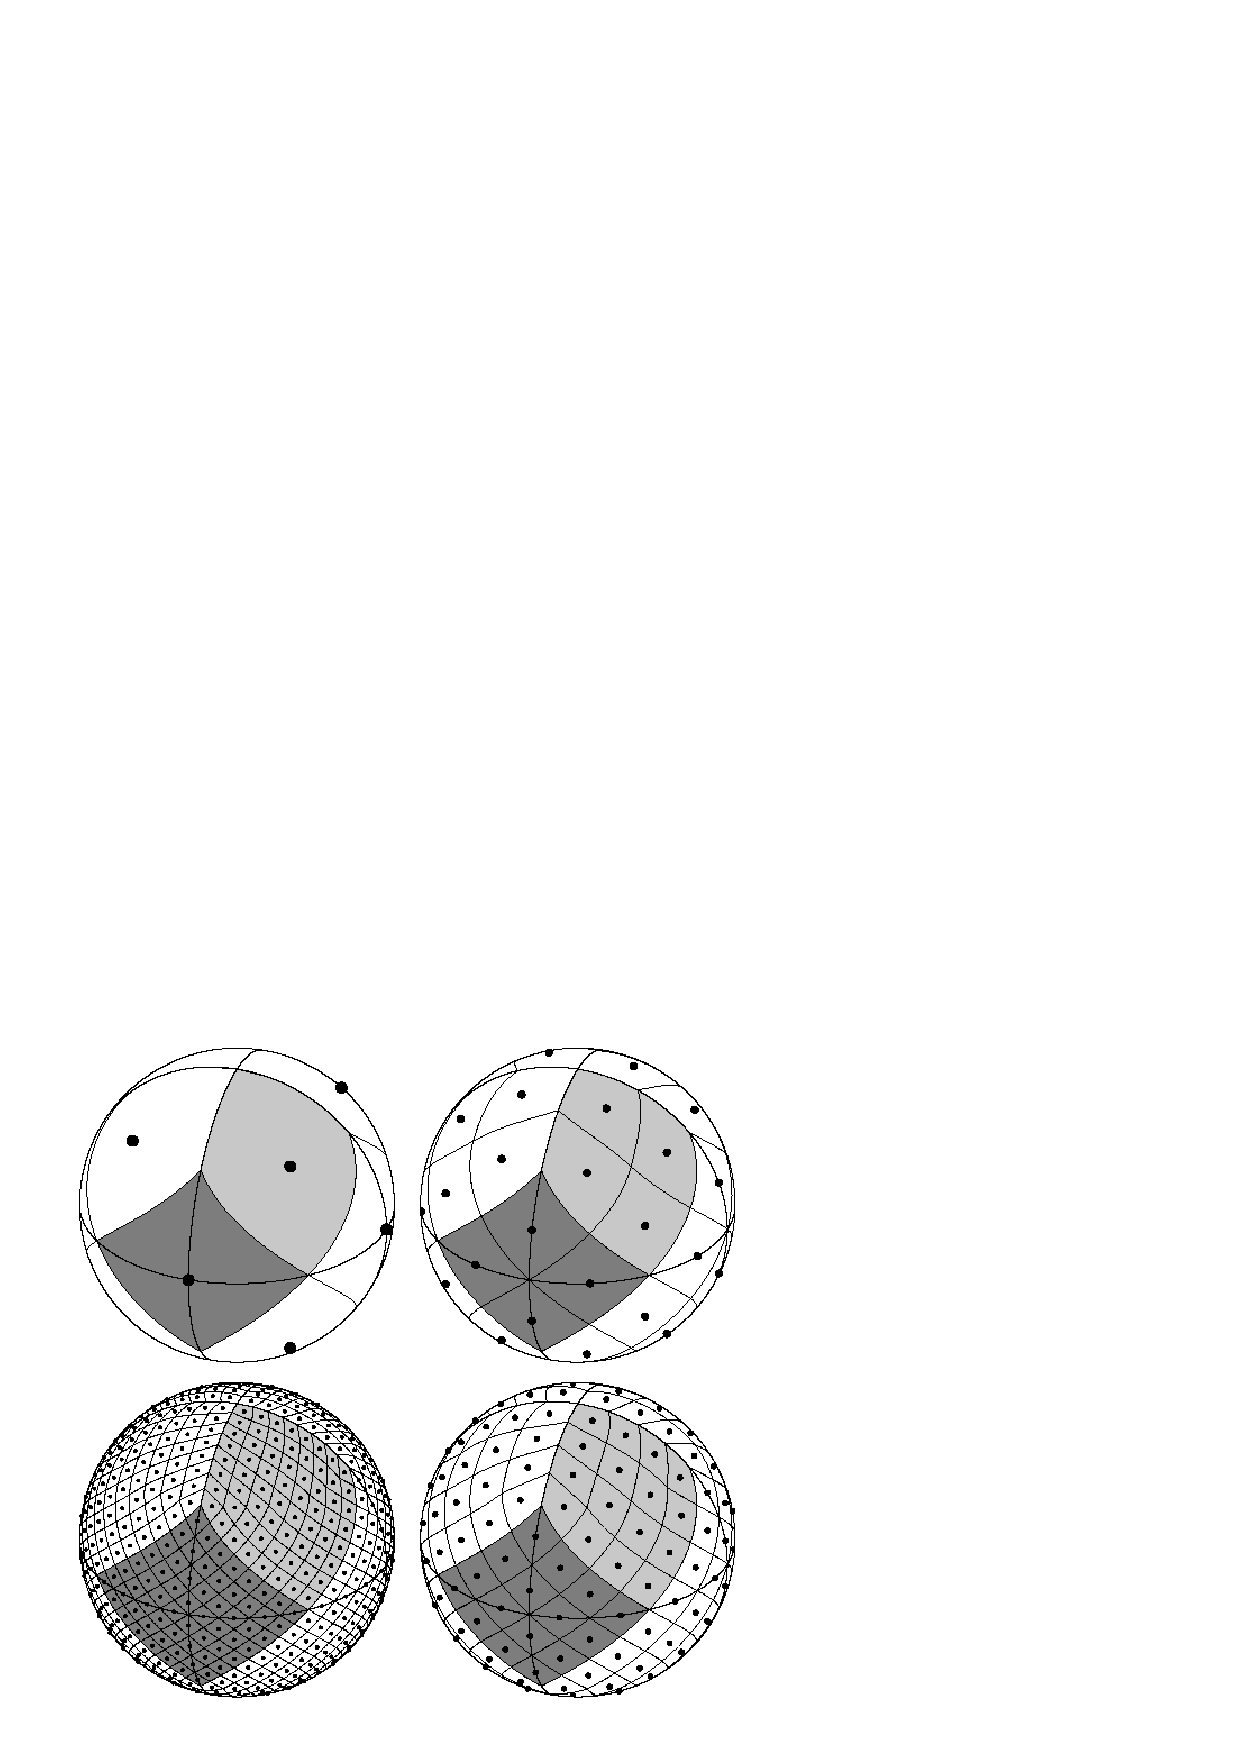
\includegraphics{pixelhealpix}
\caption{The Healpix sampling grid.}
\label{pixelhealpix}
\end{figure}

An important geometrical feature of the Healpix sampling grid is the hierarchical quadrilateral tree structure. This defines a \emph{natural} 
one-to-one mapping of the sphere sampled according to the Healpix grid, into twelve \emph{flat} images, on all scales. It is then easy to 
partition a spherical map using Healpix into quadrilateral blocks of a specified size. One first extracts the twelve base-resolution faces, 
and each face is then decomposed into overlapping blocks of the specified size. This decomposition into blocks is an essential step of the 
traditional \emph{flat} 2D curvelet transform. Based on the reversible warping of the sphere into a set of flat images made possible by the 
Healpix sampling grid, the ridgelet and curvelet transforms can be extended to the sphere. 

With the decomposition into blocks described above, there is no overlapping between neighboring blocks belonging to different base-resolution faces. 
This may result for instance in blocking effects in denoising experiments \emph{via} non linear filtering. It is possible to overcome this difficulty 
in some sense by working simultaneously with various rotations of the data with respect to the sampling grid. This will average out undesirable 
effects at edges between base resolution faces. 

\section{Multiscale methods on the sphere}

\subsection{Wavelets on the sphere}

In the last years, several wavelet transforms on the sphere have been proposed. Schr{\"o}der and Sweldens \cite{wave:sweldens95a} have developed 
an orthogonal wavelet transform on the sphere based on the Haar wavelet function which then suffers from the poor properties of the Haar function 
and the problems inherent to the orthogonal decomposition. A few papers describe continuous wavelet transforms on the sphere \cite{wave:antoine99,wave:tenerio99,wave:cayon01,wave:holschneider96}. 
An application to the detection of non-Gaussianity in the CMB radiation using the stereographic Mexican hat wavelet is reported in \cite{wave:vielva04}. 
These methods have been extended to directional wavelet transforms \cite{wave:antoine01,wave:hobson04,wave:wiaux}. Although profitable for data 
analysis, these continuous transforms lack an inverse transform and hence are clearly not suitable for restoration purposes. The algorithm proposed 
by Freeden and Maier\cite{freeden97,freeden98}, based on the Spherical Harmonic Decomposition, is to our knowledge the only one to have an inverse transform.\\  

A very popular wavelet algorithm in astrophysical applications is the so-called ``\emph{\`a trous} algorithm'' (a better name would be the 
``isotropic undecimated wavelet transform'' ), which possesses the following features: i) it is isotropic, ii) it is undecimated, iii) it uses 
an order three Box-Spline as scaling function. The isotropy of the wavelet function makes this decomposition optimal for the detection of 
isotropic objects. The non decimation makes the decomposition redundant (the number of coefficients in the decomposition is equal to the number 
of samples in the data multiplied by the number of scales) and allows us to avoid Gibbs aliasing after reconstruction in image restoration 
applications, as generally occurs with orthogonal or bi-orthogonal wavelet transforms. The choice of a $B_3$-spline is motivated by the fact 
that we want an analyzing function close to a Gaussian, but verifying the dilation equation, which is required in order to have a fast transformation. 
Finally the last property of this algorithm is to provide a very straightforward reconstruction. Indeed, the sum of all the wavelet scales and 
of the coarsest resolution image reproduces exactly the original image. \\

The \mrs package offers an implementation of a new isotropic wavelet transform on the sphere. Its properties are similar to those of the \emph{\`a trous} 
algorithm and therefore should be very useful for data denoising and deconvolution. This algorithm, described in chapter~\ref{ch_mms}, is directly derived
from the FFT-based wavelet transform proposed in\cite{starck:sta94_3} for aperture synthesis image restoration. It is relatively close to the Freeden and 
Maier \cite{freeden98} method, except that the reconstruction process is as straightforward as in the \emph{\`a trous} algorithm (i.e. the sum of the scales 
reproduces the original data). This new wavelet transform can also be easily extended to a pyramidal wavelet transform, which may be very important for 
larger data sets such such as from the future Planck experiment.

\subsection{Ridgelets and Curvelets on the sphere}
 
When analyzing data which contains anisotropic features, wavelets are no longer optimal. This has motivated the development of new multiscale 
decompositions such as the ridgelet and the curvelet transforms \cite{cur:donoho99,starck:sta01_3}. Among possible applications of those data 
analysis methods, it was shown in Starck et al. \cite*{starck:sta03_1} that the \emph{flat} curvelet transform could be useful for the detection 
of non Gaussianity in \emph{flat} patches of CMB data, and also to discriminate among different causes of non Gaussianity. 

In this area, further insight will come from the analysis of full-sky data mapped to the sphere thus requiring the development of a curvelet 
transform on the sphere. The \mrs package offers an implementation of ridgelet and curvelet transforms for spherical maps. Those implementations 
are derived as extensions of the digital ridgelet and curvelet transforms described in \cite{starck:sta01_3}. The implemented undecimated isotropic 
wavelet transform on the sphere and the specific geometry of the Healpix sampling grid are important components of the present implementation of 
curvelets on the sphere. \\
 
Further motivation for developing these new multiscale methods on the sphere follows from the results obtained in different data processing applications. 
As described in chapter\ref{ch_restore}, the \mrs package provides the necessary tools to experiment with these new spherical multiscale transforms in 
denoising applications, for instance using the Combined Filtering Method, which allows us to filter data on the sphere using both the Wavelet and the 
Curvelet transforms. The analysis of multichannel data mapped to the sphere, a problem encountered for instance in the processing of WMAP and Planck 
observations, is another issue that is shown to benefit from the developed multiscale representations on the sphere. This is reported in chapter~\ref{ch_mrs_ica} 
which is dedicated to describing some methods in multichannel data analysis extended to spherical maps which are implemented in the \mrs package.  
 
\section{Processing of polarized datas on the sphere}

Polarized maps are a special kind of multi-dimentionnal datas with strong links between their components. The polarization is of great importance 
in physics or astrophysics as it's analysis denotes fundamentals characteristics of the observed object or phenomenum. An example of great interest 
is today the cosmic microwave background \cite{starck}.

The statistical analysis of the slight intensity fluctuations in the primordial cosmic microwave background radiation field, for which evidence was 
found for the first time in the early 1990's in the observations made by COBE~\cite{gauss:smoot92}, is a major issue in modern cosmology as these 
are strongly related to the cosmological scenarios describing the properties and evolution of our Universe. In the Big Bang model, the observed CMB 
anisotropies are an imprint of primordial fluctuations in baryon-photon density from a time when the temperature of the Universe was high enough above 
3000~K for matter and radiation to be tightly coupled. At that time, the attraction of gravity and the repulsive radiation pressure were opposed, thus 
generating so-called acoustic oscillations in the baryon-photon fluid, causing peaks and troughs to appear in the power spectrum of the spatial anisotropies 
of the CMB. With the Universe cooling down as it expanded, matter and radiation finally decoupled. Photons were set free in a nearly transparent Universe, 
while the density fluctuations collapsed under the effect of gravity into large scale structures such as galaxies or clusters of galaxies. Due to the 
expansion of the Universe, the CMB photons are now observed in the microwave range but are still distributed according to an almost perfect black body 
emission law. Another major result was the measurement of the polarization state and anisotropies of the CMB radiation field by DASI~\cite{dasi}. 
Only a fraction of the total CMB radiation is polarized so that extremely sensitive instruments are needed. Polarization of the CMB radiation is a 
consequence of the Thomson scattering of photons on electrons. But for the outgoing population of photons to be polarized, the radiation incident on 
the scatterer needs to be anisotropic and have a quadrupole moment. The statistics of the CMB polarization anisotropies are also a source of information 
for cosmology. Inference of cosmological parameters from the joint statistics of the CMB anisotropies should benefit from both the complementarity and 
the redundancy of the information carried by the additional measurement of CMB polarization. Hence the full-sky maps with unprecedented sensitivity and 
angular resolution of both temperature and polarization anisotropies of the CMB to be delivered by the upcoming Planck Surveyor satellite experiment are 
awaited with excitement.

\subsection{Orthogonal representation of polarized datas}
\label{sec:polar}

\begin{figure*}[htb]
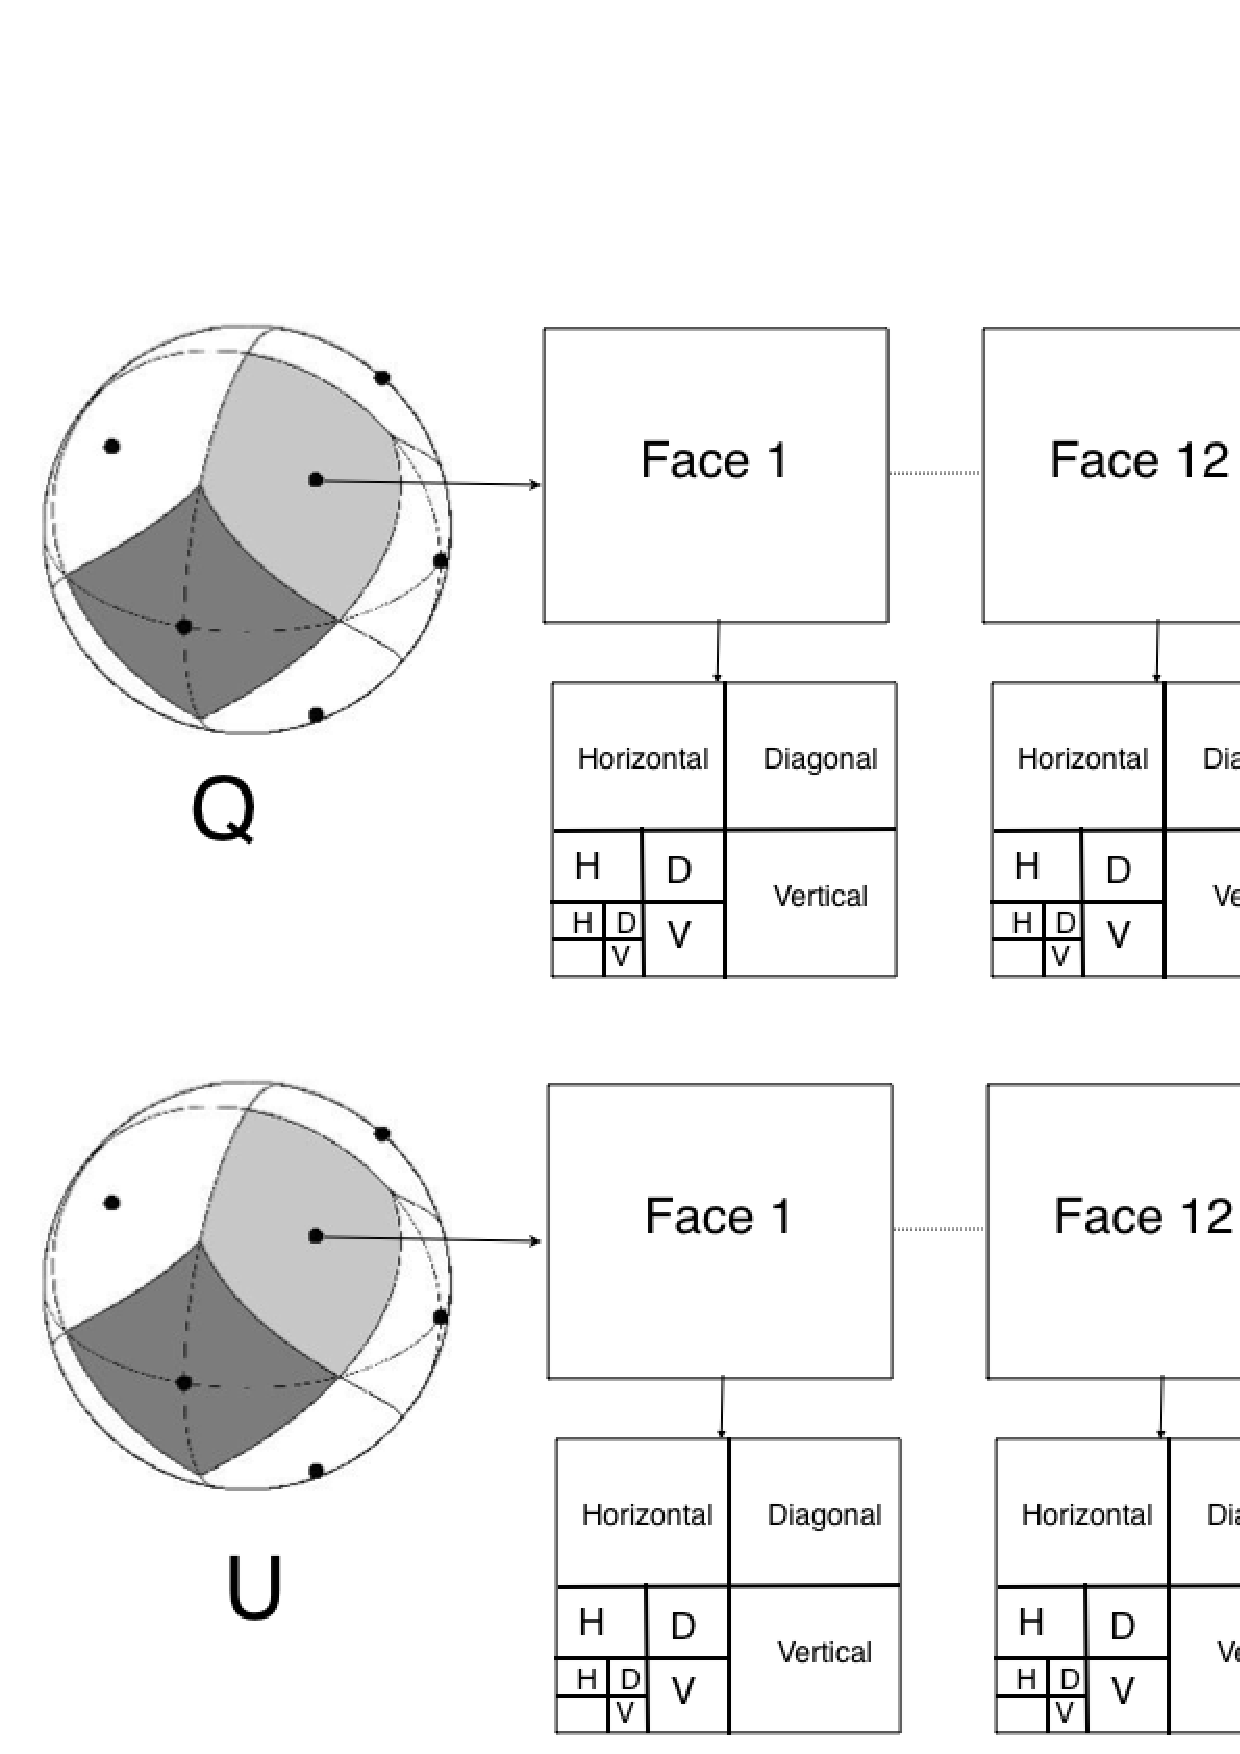
\includegraphics[width=\textwidth]{fig_pola_qu_owt_trans.pdf}
\caption{Q-U orthogonal Wavelet Transform.}
\label{fig_qu_owt_trans}
\end{figure*}
Full-sky CMB polarization data, as expected from the upcoming Planck experiment, consists of measurements of the Stokes parameters so that in addition 
to the temperature $T$ map, $Q$ and $U$ maps are given as well. The fourth Stokes parameter commonly denoted $V$ is a measure of circular polarization. 
In the case of CMB which is not expected to have circularly polarized anisotropies, $V$ vanishes. The former three quantities, $T$, $Q$ and $U$ then 
fully describe the linear polarization state of the CMB radiation incident along some radial line of sight : $T$ is the total incoming intensity, $Q$ is 
the difference between the intensities transmitted by two perfect orthogonal polarizers the directions of which define a reference frame in the tangent 
plane, and $U$ is the same as $Q$ but with polarizers rotated 45 degrees in that tangent plane. Clearly, $Q$ and $U$ are not invariant through a rotation 
of angle $\phi$ of the local reference frame around the line of sight. In fact, it is easily shown that~:
\begin{eqnarray}
Q ' = & \cos (2 \phi) Q + \sin(2 \phi) U \\ \nonumber
U ' = & \cos (2 \phi) U - \sin(2 \phi) Q 
\end{eqnarray}
which can also be written $Q' \pm i U' = e^{\mp i\phi} ( Q \pm i U )$ which by definition expresses the fact that the quantities $Q \pm i U$ are 
spin-2 fields on the sphere. The suitable generalization of the Fourier representation for such fields is the spin-2 spherical harmonics basis 
denoted $_{\pm 2}Y_{\ell m}$, in which we can expand~: 
\begin{eqnarray}\label{QU}
Q \pm i U  = \sum_{\ell, m} { _{\pm 2}a_{\ell m}} {_{\pm 2}Y_{\ell m} }
\end{eqnarray}

It is convenient~\cite{zalda} to introduce the two quantities denoted $E$ and $B$ which are defined on the sphere by~:
\begin{eqnarray}\label{EB}
E = & \sum_{\ell, m} a_{\ell m} ^E Y_{\ell m} = \sum_{\ell, m} - \frac{1}{2} ( {_{ 2}a_{\ell m}} + {_{- 2}a_{\ell m}} ) Y_{\ell m} \\ \nonumber
B = & \sum_{\ell, m} a_{\ell m} ^B Y_{\ell m} = \sum_{\ell, m} i \frac{1}{2} ( {_{ 2}a_{\ell m}} - {_{- 2}a_{\ell m}} ) Y_{\ell m} 
\end{eqnarray}

\subsection{Multiscale transform on the sphere for polarized datas}

Inprovements in the second version of the \mrs package includes extension of the 1D multiscale transforms to the case of polarized maps with 
the three fields $T$, $Q$ and $U$ (or the fields $T$, $E$ and $B$). The easiest way to build a multiscale transform for polarized data is to 
use the Healpix\footnote{http://healpix.jpl.nasa.gov} representation \cite{pixel:healpix}, and to apply a bi-orthogonal wavelet transform 
on each face of the Healpix map, separately for $Q$ and $U$. Fig.~\ref{fig_qu_owt_trans} shows the flow-graph of this Q-U orthogonal wavelet 
transform (QU-OWT). Most of the algorithms included in \mrs for the processing of 1D images know have a version for polarized maps.

% \clearpage
% \newpage


\include{multicale}

% Filtering chapter


\chapter[ICA on the Sphere]{Independent Component Analysis on the Sphere}
\label{ch_mrs_ica}


\section{Introduction}
\index{blind source separation}
\index{ICA}


Blind Source Separation (BSS) is a problem that occurs in multi-dimensional data processing. The overall goal is to recover 
unobserved signals, images or \emph{sources} $S$ from mixtures of these sources $X$ observed typically at the output of an 
array of sensors. The simplest mixture model takes the form:
\begin{equation}\label{model0}
X = A S
\end{equation}
where $X$ and $S$ are random vectors of respective sizes $m \times 1$, $n \times 1$ and $A$ is an $m \times n$ matrix. The 
entries of $S$ are assumed to be independent random variables. Multiplying $S$ by $A$ linearly mixes the $n$ sources into 
$m$ observed processes. \\ 
   
Independent Component Analysis methods were developed to solve the BSS problem, \emph{i.e.} given a batch of $T$ observed 
samples of $X$, estimate the mixing matrix $A$ and reconstruct the corresponding $T$ samples of the source vector $S$, relying 
mostly on the statistical independence of the source processes. Note that with the above model, the independent sources can 
only be recovered up to a multiplication by a \emph{non-mixing} matrix \emph{i.e.} up to a permutation and a scaling of the 
entries of $S$. Although independence is a strong assumption, it is in many cases physically plausible. The point is that 
it goes beyond the simple second order decorrelation obtained for instance using Principal Component Analysis (PCA) : decorrelation 
is not enough to recover the source processes since any rotation of a white random vector remains a white random vector.\\


Algorithms for blind component separation and mixing matrix estimation depend on the model used for the probability distribution 
of the sources~\cite{ica:3easy}. In a first set of techniques, source separation is achieved in a noise-less setting, based on the 
non-Gaussianity of all but possibly one of the components. Most mainstream ICA techniques belong to this category : JADE~\cite{ica:jade}, 
FastICA, Infomax~\cite{ica:icabook}. In a second set of blind techniques, the components are modeled as Gaussian processes, either 
stationary or non stationary and, in a given representation, separation requires that the sources have diverse, \emph{i.e.} non 
proportional, variance profiles. The Spectral Matching ICA method (SMICA) ~\cite{ica:Del2003}, considers in this sense the case of 
mixed stationary Gaussian components and goes further than the above model (Eq.~\ref{model0}) by taking into account additive 
\emph{instrumental } noise $N$:
\begin{equation}\label{model1}
X = A S + N
\end{equation}
Moving to a Fourier representation, the idea is that colored components can be separated based on the diversity of their power spectra.\\ 
 
The next two sections give a short overview of two significant ICA methods mentioned above and implemented in the \mrs package: 
JADE and SMICA. A shorter description of FastICA ~\cite{ica:icabook} is also given. This is followed by a description of ways to 
combine wavelets and ICA techniques. Some useful properties of wavelet transforms can indeed come enhance the performance of ICA 
methods in several situations. 

    
\section{JADE}
\index{ICA!jade}

The Joint Approximate Diagonalization of Eigenmatrices method (JADE) assumes the observed data $X$ follows the noiseless mixture 
model~(\ref{model0}) where the independent sources $S$ are non-Gaussian \emph{i.i.d.}\footnote{The letters \emph{i.i.d.} stand for 
independently and identically distributed meaning that each entries of $X$ at a given time $t$ are independent of $X$ at any other 
time $t'$ and that the distribution of $X$ does not depend on time. } random processes. The mixing matrix is assumed to be square 
and invertible so that (de)mixing is actually just a change of basis.

As mentioned above, second order statistics do not retain enough information for source separation in this context: finding a change of 
basis in which the data covariance matrix is diagonal will not in general enable to identify the independent sources properly. Nevertheless, 
decorrelation is \emph{half the job}~\cite{ica:tutorial} and one may seek the basis in which the data is represented by maximally independent 
processes among those bases in which the data is decorrelated. This leads to so-called orthogonal algorithms: after a proper whitening of 
the data by multiplication with the inverse of a square root of the covariance matrix of the data $W$, one is then seeking a rotation $R$ 
(which leaves things white) so that $\hat{ S}$ defined by
\begin{equation}
\hat{ S} = W^{-1} \, Y =  W^{-1}\, R \, X_{\textrm{white}}  = W^{-1}\, R \, W \, X 
\end{equation}
and $\hat{B} = \widehat{A^{-1}} =  W^{-1}\, R \, W$ are estimations of the sources and of the inverse of the mixing matrix.\\

JADE is such an orthogonal ICA method and, like most mainstream ICA techniques, it exploits higher order statistics so as to achieve some 
sort of \emph{ non linear decorrelation}. Precisely, in the case of JADE, statistical independence is assessed using fourth order cross cumulants : 
\begin{eqnarray}  \nonumber	 
F_{ijkl} & = & \textrm{cum}( y_i, y_j, y_k, y_l )   \nonumber    \\
  & =& \mathcal{E} (y_i y_j y_k y_l) - \mathcal{E} (y_i y_j)\mathcal{E} (y_k y_l)\nonumber \\
  & & -\mathcal{E} (y_iy_l)\mathcal{E} ( y_j y_k)-\mathcal{E} (y_iy_k)\mathcal{E} (y_j y_k)
\end{eqnarray}
where $\mathcal{E}$ stands for statistical expectation and the $y_i$'s are the entries of vector $Y$ modeled as random variables, 
and the correct change of basis (\emph{i. e.} rotation) is found by somehow \emph{diagonalizing} the fourth order cumulant tensor. 
Indeed, if the $y_i$'s were independent, all the cumulants with at least two different indices would be zero. As a consequence of 
the independence assumption of the source processes $S$ and of the \emph{whiteness} of $Y$ for all rotations $R$, the fourth order 
tensor $F$ is well structured: JADE was precisely devised to take advantage of the algebraic properties of $F$. JADE's objective 
function is given by
\begin{eqnarray}  \nonumber	 
%\mathcal{J}_{\textrm{jade}}( R )   &=& \sum _{ijkl \ne ijkk}  \textrm{cum}(  y_i, y_j, y_k, y_l )^2  \nonumber    \\
  \mathcal{J}_{\textrm{jade}}( R ) & =&  \sum _{ij}   \sum_{k \ne l} \textrm{cum}(  y_i, y_j, y_k, y_l )^2  
\end{eqnarray}
which can be interpreted as a joint diagonalization criterion. Fast and robust algorithms are available for the minimization 
of $\mathcal{J}_{\textrm{jade}}( R )$ with respect to $R$ based on Jacobi's method for matrix diagonalization~\cite{ica:pham2001}. 
More details on JADE can be found in~\cite{ica:jade,ica:tutorial,ica:icabook}.


\subsubsection{JADE for spherical maps}

Applying JADE on multichannel data mapped to the sphere does not require any particular modification of the algorithm. Indeed, JADE estimates 
the fourth order cumulant tensor from the available data samples assuming an \emph{i.i.d.} random field. Hence, given a pixelization scheme on 
the sphere such as provided by the Healpix package, JADE can be directly applied to the multichannel spherical data pixels.


\section{FastICA}
\index{ICA!fastica}

FastICA is by now a standard technique in ICA. Like JADE, it is meant for the analysis of mixtures of independent non-Gaussian sources in 
a noise-less setting. A complete description of this method can be found in \cite{ica:icabook} and references therein. Many papers on this 
algorithm are available at \emph{http://www.cs.helsinki.fi/ u/ahyvarin/papers/fastica.shtml}. We give here a brief and simplified account 
of the algorithm. FastICA, again like JADE, is a so-called orthogonal ICA method: the independent components are sought by maximizing a 
measure of non-Gaussianity under the constraint that they are decorrelated. Intuitively, one should understand that mixtures of independent 
non-Gaussian random variables tend to \emph{ look more Gaussian}. An enlightening view on the relation between mutual information, which is 
a natural measure of independence, decorrelation and non-Gaussianity can be found in~\cite{ica:3easy,ica:geomindep}. Non-Gaussianity is assessed 
in FastICA using a contrast function $G$ based on a non-linear approximation to \emph{negentropy}~\cite{ica:icabook}. In practice, depending 
on the application, different approximations or non-linear (non-quadratic) functions should be experimented with. In a simple deflation scheme, 
for sphered data, the directions are found sequentially : a direction $r$ of maximal non-Gaussianity is sought by maximizing 
\begin{equation}
J_G(r) = \Big( \mathcal{E} \{ G(r^T x_{\textrm{white}}  ) \} - \mathcal{E} \{ G(\nu ) \} \Big)^2 
\end{equation}
where $\nu$ stands for centered unit variance Gaussian variable, under the constraint that $r$ has unit norm and that $r$ is orthogonal 
to the directions found previously. The contrast function $G$ can for instance be chosen among the following~\cite{ica:icabook}:
\begin{eqnarray}
G_0 (u)  & = &  \frac{1}{a} \textrm{log}\,\textrm{cosh} (a u ) \nonumber    \\
G_1 (u)  & = &  -\frac{1}{a} \textrm{exp}(- a u^2 / 2 )   \nonumber	   \\
G_2 (u)  & = &  \frac{1}{4} u^4 \nonumber    \\
\end{eqnarray}
where $a$ is a constant to be determined depending on the application. It can be shown that the maxima of $J_G$ occur at certain maxima 
of $\mathcal{E} \{ G(r^T x_{\textrm{white}} ) \} $. These are obtained for $r$ solution to :
\begin{equation}
\mathcal{E} \{ x_{\textrm{white}} g(r^T x_{\textrm{white}}  ) \} - \lambda r = 0 
\end{equation}
where $\lambda$ is a constant easily expressed in terms of the optimal direction $r_0$, and $g$ is the derivative of $G$. Solving this 
equation using Newton's method, and a few approximations, a \emph{fixed-point} algorithm is derived which consists in repeating the 
following two steps until convergence :
\begin{eqnarray}
r  & \leftarrow & \mathcal{E} \{ x_{\textrm{white}} g(r^T x_{\textrm{white}}  ) \} - \mathcal{E} \{ g'(r^T x_{\textrm{white}}  ) \} r     \nonumber  \\
r  & \leftarrow  &  \frac{r}{\| r \|}   \nonumber	   \\
\end{eqnarray}
A simple implementation of this algorithm is included in the present package. It is largely based on the $\textbf{Matlab}^{TM}$ code 
available at \emph{www.cis.hut.fi/projects/ica/fastica/}. 

%\section{SMICA}
%\index{smica}
%\index{ICA!smica}
%
%Spectral Matching ICA (SMICA) was designed to address some of the general problems raised by Cosmic Microwave Background data analysis 
%where the major component of interest (CMB itself) is well modeled by an isotropic stationary Gaussian random field. Although standard 
%ICA methods may be used in this context, they are not expected to perform as well as methods based on Gaussian model especially in the 
%presence of additive Gaussian instrumental noise as in (\ref{model1}).   
%
%SMICA belongs to a set of blind source separation techniques where the components are modeled in a given representation as \emph{locally i.i.d.} 
%centered Gaussian processes. Independent Gaussian sources can then be separated based on their statistical independence (which obviously reduces 
%\emph{locally} to decorrelation) provided they have diverse (\emph{i.e.} non proportional) variance profiles \emph{i.e.} energy distributions in 
%that representation. SMICA considers in this sense the case of mixed stationary Gaussian components in a noisy context as in model~(\ref{model1}) : 
%moving to a Fourier representation, colored components can be separated based on the diversity of their power spectra. 
%
%\subsection{SMICA's objective function} 
%
%In order to derive the Spectral Matching ICA criterion, we assume that, in the Fourier domain, the \emph{locally i.i.d.} Gaussian sources $S$ 
%and noise $N$ processes in (\ref{model1}) actually have constant spectral covariance matrices $R_f^S(q) \in \mathbb{R}^{n\times n}$ and $R_f^N(q) 
%\in \mathbb{R}^{m \times m} $ on each of a set of $Q$ frequency bands. Clearly, the appropriate notion of frequency should be used, depending on 
%whether the data $X$ is a set of time series, a set of 2D maps, etc. The assumption of statistical independence between the components $S$ implies 
%that the $R_f^S(q)$ are diagonal matrices. With a similar assumption regarding  the noise processes in the $m$ different channels, the $R_f^N(q)$ 
%also are diagonal matrices. Applying a Fourier transform on (\ref{model1}) does not affect the mixing matrix $A$, so that the model covariance 
%matrix of the observations $X$ in the $q^{\textrm{th}}$ frequency band is structured as  
%\begin{equation}
%\label{structure}
%R_f^X(q) = A R_f^S(q) A^{\dagger} +   R_f^N(q)
%\end{equation}
%where we assumed that the instrumental noise is independent of the sources. Then, provided estimates $\widehat{R}_f^X(q) $ of $R_f^X(q) $ can be 
%obtained from the available data (\emph{e.g.} empirical covariance estimator), SMICA consists in minimizing 
%\begin{equation}\label{Cost_fourier}
% \Phi_f (\theta) =  \sum _{q=1}^{Q}  \alpha_q \mathcal{D} \left( \widehat{R}_f^X(q) \ , A R_f^S(q) A^{\dagger} +   R_f^N(q) \right)
%\end{equation}
%for some sensible choice of the weights $\alpha_q$ and of the matrix mismatch measure $\mathcal{D}$, with respect to the full set of parameters 
%$\theta = (A,R_f^S(q), R_f^N(q) )$ or a subset thereof. As discussed in ~\cite{ica:Del2003}, a good choice for $\mathcal{D}$ is
%\begin{equation}\label{eq:kl}
%  \mathcal{D}_{KL} (R_1, R_2 )  =  \frac{1}{2} \Big( \mathrm{tr} (R_1R_2^{-1}) - \log\det (R_1R_2^{-1}) - m  \Big)
%\end{equation}
%which is the Kullback-Leibler divergence between two $m$-variate zero-mean Gaussian distributions with covariance matrices $R_1$ and $R_2$. 
%With this mismatch measure, the SMICA criterion is shown to be related to the likelihood of the data in a Gaussian model, so that we can resort 
%to the EM algorithm to minimize~(\ref{Cost_fourier}). The weights $\alpha_q$ should be chosen to reflect the variability of the estimate of the 
%corresponding covariance matrix. Following the derivation in~\cite{ica:Del2003}, these are taken to be the number of Fourier modes in each band $q$. \\
%
%\subsection{Source map estimation}\label{sect:mapesti}
%
%As a result of applying SMICA, power densities in each frequency band are estimated for the sources and detector noise along with 
%the estimated mixing matrix. These may be used in reconstructing the source maps \emph{via} for instance Wiener filtering in each band: 
%a Fourier mode $X(\nu)$ in frequency band $q$ is used to reconstruct the maps according to
%\begin{equation}
%  \widehat{S}(\nu) 
%  =
%  (\widehat{A}\adj \widehat{R}_f^N(q)^{-1} \widehat{A} + \widehat{R}_f^S(q)^{-1})\inv 
%  \widehat{A}\adj \widehat{R}_f^N(q)^{-1} X(\nu)
%  \label{Wiener}
%\end{equation}
%In the limiting case where noise is small compared to signal components, this filter reduces to 
%\begin{equation}
% \widehat{S}(\nu)  =
%  (\widehat{A}\adj \widehat{R}_f^N(q)^{-1} \widehat{A} )\inv 
%  \widehat{A}\adj \widehat{R}_f^N(q)^{-1} X(\nu)
%  \label{Wiener1}
%\end{equation}
%Clearly, the above Wiener filter is optimal only in front of stationary Gaussian processes. For non Gaussian maps, such as given by 
%the Sunyaev Zel'dovich effect, better reconstruction can be expected from non linear methods.
%
%\subsection{SMICA for spherical maps}\label{sect:smicas}
%
%In the linear mixture model~(\ref{model1}), $X$ now stands for an array of observed spherical maps, $S$ is now an array of spherical source maps 
%to be recovered and $N$ is an array of spherical noise maps. The mixing matrix $A$ achieves a pixelwise linear mixing of the source maps, in the 
%Healpix scheme for instance.
% 
%Extending SMICA to deal with multichannel data mapped to the sphere is straightforward~\cite{ica:Del2003}. The idea is simply to substitute the 
%spherical harmonics transform to the Fourier transform used in the above description of SMICA. Then, data covariance matrices are estimated in 
%this representation over $Q$ intervals in multipole number $l$, assuming the components are stationary and isotropic over the sphere. These $Q$ 
%covariance matrices are still structured according to~(\ref{structure}) and source separation can be achieved by minimizing the spectral matching 
%criterion~(\ref{Cost_fourier}). Source maps reconstruction follows as in section~\ref{sect:mapesti}.\\
%
%SMICA has already been applied in astrophysical data analysis, showing significant success for CMB spectral estimation in multidetector 
%experiments~\cite{ica:Del2003,ica:patanchon}. Working in the frequency domain does offer several benefits such as easy handling of detector 
%dependent point spread functions. However, the non locality of the Fourier or the spherical harmonics transform will have some undesired 
%effects when dealing with non-stationary components or noise, or with incomplete data maps. The latter is a common issue in astrophysical 
%data analysis : either the instrument scanned only a fraction of the sky or some regions of the sky were masked due to localized strong 
%astrophysical sources of contamination (compact radio-sources or galaxies, strong emitting regions in the galactic plane). A simple way 
%to overcome these effects is to move instead to a wavelet representation so as to benefit from the localization property of wavelet filters. 
%This leads to WSMICA~\cite{starck:yassir05}, an extension of SMICA which is reviewed in section~\ref{sect:wsmica} below. 



\section{ICA and Wavelets} 
\index{wavelet!ICA}
\index{ICA!wavelet}


Several properties of wavelets have been recognized as particularly useful in multichannel data processing : bringing wavelets and 
independent component analysis together has proven quite profitable. Extensions WJADE and WSMICA of the two ICA methods described 
previously are discussed in this section.

Wavelets are remarkable at data compression meaning data that is structured in the initial representation requires fewer significant 
coefficients in a wavelet representation. In imprecise and general terms, wavelets grab the coherence between coefficients of the 
structured data and produces a smaller set of significant coefficients which are then less coherent and which have a sparser statistical 
distribution. Then, the super-Gaussian\footnote{A super-Gaussian distribution is also called a lepto-kurtic distribution, referring to a 
distribution with a narrow central peak and heavy tails. A typical example is the Laplacian distribution.} \emph{i.i.d.} statistical model 
which appears in most standard ICA methods may better suit the wavelet coefficients of the data than the data samples in the initial representation. 

Wavelets have been developed for the analysis of non-stationary and singular data in order to overcome certain difficulties attached to 
the Fourier transform. Wavelets are widely used to reveal variations in the spectral content of time series or images as they permit to 
single out regions in direct space while retaining localization in the frequency domain. Astrophysical data analysis has much to gain in 
avoiding the assumption of stationarity underlying Fourier analysis. Moreover, observed data maps are commonly imperfectly shaped and 
incomplete with missing or masked patches due to experimental settings, scanning strategies, etc. This will impair direct application of 
the Spectral Matching ICA method described previously. One might consider resorting to wavelets.     
          
 
%In dealing with non stationary data or incomplete data, an attractive feature of  wavelet filters over the spherical harmonic transform is that they are well localized in the initial representation. 

%Dealing with non stationary data or incomplete data is made simpler due to the good localization of wavelet coefficients in the initial representation.In the smaller scales, most of the samples in the filtered signal will  be unaffected by the presence of gaps and only these samples should be used to estimate the data covariance matrices on each wavelet scale.

\subsection{WJADE}\label{sec:wjade}
\index{ICA!wjade}
\index{jade!wavelet}

Wavelets come into play as a sparsifying transform. Applying a wavelet transform on both sides of~(\ref{model0}) does not affect the 
mixing matrix and the model structure is preserved. Also, moving the data to a wavelet representation does not affect its information 
content. However, the statistical distribution of the data coefficients in the new representation is different: wavelets are known to 
lead to sparse \emph{i.i.d.} representations of structured data. Further, the \emph{local} (coefficient wise) signal to noise ratio 
depends on the choice of a representation. A wavelet transform tends to grab the informative coherence between pixels while averaging 
the noise contributions, thus enhancing structures in the data. Although the standard ICA model~(\ref{model0}) is for a noiseless setting, 
the derived methods can be applied to real data. Performance will depend on the detectability of significant coefficients \emph{i.e.} on 
the sparsity of the statistical distribution of the coefficients. Moving to a wavelet representation will often lead to more robustness to noise.    

Once the data has been transformed to a proper representation (\emph{e.g.} wavelets but also ridgelets and curvelets in the case of strongly 
anisotropic 2D or 3D data), WJADE consists in applying the standard JADE method to the new multichannel coefficients. Once the mixing matrix 
is estimated, the initial source maps are obtained using the adequate inverse transform after some non linear denoising or thresholding of 
the coefficients if necessary.

\subsection{Covariance matching in wavelet space : WSMICA}\label{sect:wsmica}
\index{ICA!wsmica}
\index{smica!wavelet}
\index{wavelet!transform}

Let us consider the case of spherical maps as in \ref{sect:smicas} but possibly incomplete, partly masked or non-stationary. As a model case, 
we actually consider incomplete data maps in which the positions of the missing pixels are known in advance. Moving to a wavelet representation, 
it is possible to keep track of the missing pixels on each scale so that we can derive a covariance matching ICA criterion, WSMICA, robust to 
gaps in the data. Indeed, an attractive feature of wavelet filters over the spherical harmonic transform is that they are well localized in the 
initial representation. Provided the wavelet filter response on scale $j$ is short enough compared to data size and gap widths, most of the 
samples in the filtered signal will then be unaffected by the presence of gaps. Using exclusively these samples yields an estimated covariance 
matrix $\widehat{R}_w^X(j)$ which is not biased by the missing data. The price to pay is a possibly slight increase in variance which depends on scale $j$.

With the Isotropic Undecimated Wavelet Transform on the Sphere (UWTS) decribed in section~\ref{sect_wts}, the multichannel data $X$ is decomposed 
into $J$ detail maps $X_{j}^w$ and a smooth approximation map $X_{J+1}^w$ over a dyadic resolution scale which simply sum back as: 
\begin{equation}  
X(\vartheta, \varphi) = X_{J+1}^w (\vartheta, \varphi) + \sum_{j=1}^{J} X_{j}^w(\vartheta, \varphi)
\end{equation}
Denoting $l_j$ the size of the set $\mathcal{M}_j$ of wavelet coefficients unaffected by the gaps at scale $j$, the wavelet covariances are empirically estimated using
\begin{equation}
\widehat{R}_w^X (j) = \frac{1}{l_j }  \sum_{t \in  \mathcal{M}_j } X_j^w( \vartheta_t, \varphi_t )X_j^w( \vartheta_t, \varphi_t ) ^\dagger 
\end{equation}

Clearly, applying the above UWTS on both sides of~(\ref{model1}) does not affect the mixing matrix $A$ so that 
the model covariance matrix of the observations at scale $j$, is still structured as  
\begin{equation}
R_w^X(j) = A R_w^S(j) A^{\dagger} +   R_w^N(j) 
\end{equation}
where $R_w^S(j)$ and $R_w^N(j)$ are the model diagonal spectral covariance matrices in the wavelet representation of $S$ and $N$ respectively 
at scale $j$. Given an estimation of $R_w^X(j)$ from the data, $\widehat{R}_w^X(j)$, source separation follows from  minimizing the following 
covariance matching criterion WSMICA-S in this \emph{spherical wavelets} representation:  
\begin{equation}\label{Cost_wavelet}
 \Phi (\theta) =  \sum _{j=1}^{J+1}  \alpha_j \mathcal{D} \left( \widehat{R}_w^X(j), \,
    A R_w^S(j) A^{\dagger} + R_w^N(j) \right)
\end{equation}
with respect to the full set of parameters $\theta = (A,R_w^S(j), R_w^N(j) )$ or a subset thereof. Again, a good choice for $\mathcal{D}$ is 
the Kullback-Leibler divergence given in equation~\ref{eq:kl}. With this mismatch measure, we can again resort to the EM algorithm to minimize~(\ref{Cost_wavelet}). 

The weights in the covariance mismatch~(\ref{Cost_wavelet}) should be chosen to reflect the variability of the estimate of the corresponding
covariance matrix. Since WSMICA-S uses wavelet filters with only limited overlap, in the case of complete data maps we follow the derivation 
in~\cite{ica:Del2003} and take $\alpha_j$ to be proportional to the number of spherical harmonic modes in the spectral domain covered at 
scale $j$. In the case of data with gaps, we must further take into account that only a fraction $\beta_j$ of the wavelet coefficients are 
unaffected so that the $\alpha_j$ should be modified in the same ratio. 

Source maps may be reconstructed outside the possible gaps by Wiener filtering on each scale prior to inverting the wavelet transform, following 
the procedure described in section~\ref{sect:mapesti}. Non linear filtering techniques may yield better results in the case of non-Gaussian components. 

\subsubsection{WSMICA for \emph{flat} maps}

WSMICA can be easily implemented in the case of flat 2D data maps by substituting the 2D isotropic undecimated \emph{\`a trous} algorithm with 
the cubic box-spline~\cite{starck:book02} as scaling function to the UWTS used in the previous section to deal with incomplete spherical maps.
This transform has several favorable properties for astrophysical data analysis. In particular, it is a shift invariant transform, the wavelet 
coefficient maps on each scale are the same size as the initial image, and the wavelet and scaling functions have small compact supports in the 
initial representation. As in the case of spherical maps, these properties allow  missing patches in the data maps to be handled easily.

WSMICA was used in~\cite{starck:yassir05} to process realistic CMB multichannel data as expected from the Planck experiment however on small enough 
maps so that curvature could be neglected. The reported numerical experiments clearly confirm the benefits of correctly processing existing gaps. 
Wavelets are able to correctly grab the spectral content of partly masked data maps and from there allow for better component separation.  

\section{Applications}

\subsection{CMB data analysis}\label{sect:NUMEXP}
\index{CMB}
\index{CMB!ICA}
\index{ICA!CMB}

As an application of WSMICA on the sphere, we consider here the problem of CMB data analysis but in the special case where the use of a galactic 
mask is a cause of non-stationarity which impairs the use of the spherical harmonics transform. 

The simulated CMB, galactic dust and Sunyaev Zel'dovich (SZ) maps used, shown on the left-hand side of figure~\ref{components}, were obtained as 
described in~\cite{ica:Del2003}. The problem of instrumental point spread functions is not addressed here, and all maps are assumed to have the 
same resolution.The high level foreground emissions from the galactic plane region were discarded using the $Kp2$ mask from the WMAP team 
website\footnote{\emph{http://lambda.gsfc.nasa.gov/product/map/intensity\_mask.cfm}}. These three \emph{incomplete} maps were mixed using the matrix 
in table~\ref{MatrixA}, in order to simulate observations in the six channels of the Planck high frequency instrument~(HFI).

\begin{table}[!h]
  \begin{center}
   \footnotesize {
    \begin{tabular}{@{} cccc|c @{}}
      CMB & DUST & SZ &  & channel \\
      & & & &\\
      \hline
      & & & &\\
      $\quad1.0\quad$  &  $ 1.0 $    		&  $\quad-1.51\quad$	 	&& 100~GHz\\
      $\quad1.0 \quad$ & $ 2.20$   		& $\quad-1.05\quad$  		&& 143~GHz\\
      $\quad1.0 \quad$ &  $ 7.16 $  		& $\quad0.0\quad $ 			&& 217~GHz\\
      $\quad1.0 \quad$ &   $56.96 $		&  $\quad 2.22\quad$ 	&&353~GHz\\
      $\quad1.0 \quad$ &  $1.1\times10^{3}$ 		&   $\quad5.56\quad$  	&&545~GHz\\
      $\quad1.0\quad $ &  $1.47\times10^{5}$  	& $ \quad11.03\quad $	&& 857~GHz\\
    \end{tabular}}
    \caption{Entries of $A$, the mixing matrix used in our simulations.}\label{MatrixA}
  \end{center}
\end{table}

Gaussian \emph{instrumental} noise was added in each channel according to model~(\ref{model0}). The relative noise standard deviations between channels 
were set according to the nominal values of the Planck HFI given in table~\ref{NoiseScale}. 

\begin{table}[!h]
  \begin{center}
     \footnotesize {
    \begin{tabular}{@{} cccccc|c @{}}
      100&143&217&353&545&857&channel \\
          & & & & & &\\
  \hline
          & & & & & &\\
    $ 2.65\!\!\times\!\!10^{-6}$&$2.33\!\!\times\!\!10^{-6}$&$3.44\!\!\times\!\!10^{-6}$&$1.05\!\!\times\!\!10^{-5}$&$1.07\!\!\times\!\!10^{-4}$& $4.84\!\!\times\!\!10^{-3}$ &noise std\\
          & & & & & &\\
  % \hline 
   %    & & & \\
   %   353~GHz&545~GHz  &857~GHz  &   channel\\
       %   & & &  \\
  %\hline
  %    & & & \\
   %$1.05\times10^{-5}$&$1.07\times10^{-4}$ & $4.84\times10^{-3}$ &   noise std\\
     % & & &  \\     
      \end{tabular}}
    \caption{Nominal noise standard deviations in the six channels of the Planck HFI.}\label{NoiseScale}
  \end{center}
\end{table}

The synthetic observations were decomposed into six scales using the isotropic UWTS and WSMICA was used to obtain estimates of the mixing matrix 
and of the initial source templates. The resulting component maps estimated using WSMICA, for nominal noise levels, are shown on the right-hand 
side of figure~\ref{components} where the quality of reconstruction can be visually assessed by comparison to the initial components. The component 
separation was also performed with SMICA based on Fourier statistics computed in the same six dyadic bands imposed by our choice of wavelet transform, 
and with JADE. In figure~\ref{resultats}, the performances of SMICA, WSMICA and JADE, are compared in the particular case of CMB map estimation, 
in terms of the relative standard deviation of the reconstruction error, $MQE$, defined by
 \begin{equation}
  MQE  = \frac{\mathbf{std}  ( CMB(\vartheta, \varphi)  - \alpha \times \widehat{CMB}(\vartheta, \varphi)  )}{\mathbf{std}  ( CMB(\vartheta, \varphi)   ) }
  \label{MQE}
\end{equation}  
\index{jade}
\index{smica}
\index{smica!wavelet}
\index{jade!wavelet}
where $\mathbf{std}$ stands for empirical standard deviation  obviously computed outside the masked regions), and $\alpha$ is a linear regression 
coefficient estimated in the least squares sense. As expected, since it is meant to be used in a noiseless setting, JADE performs well when noise 
is very low. However, as the noise level increases, its performance degrades quite rapidly compared to the covariance matching methods. Further, 
these results clearly show that using wavelet-based covariance matrices provides a simple and efficient way to cancel the bad impact that gaps 
have on the performance of source separation using statistics based on the non local Fourier representation. 

\begin{figure*}[htb]
% \begin{center}
% 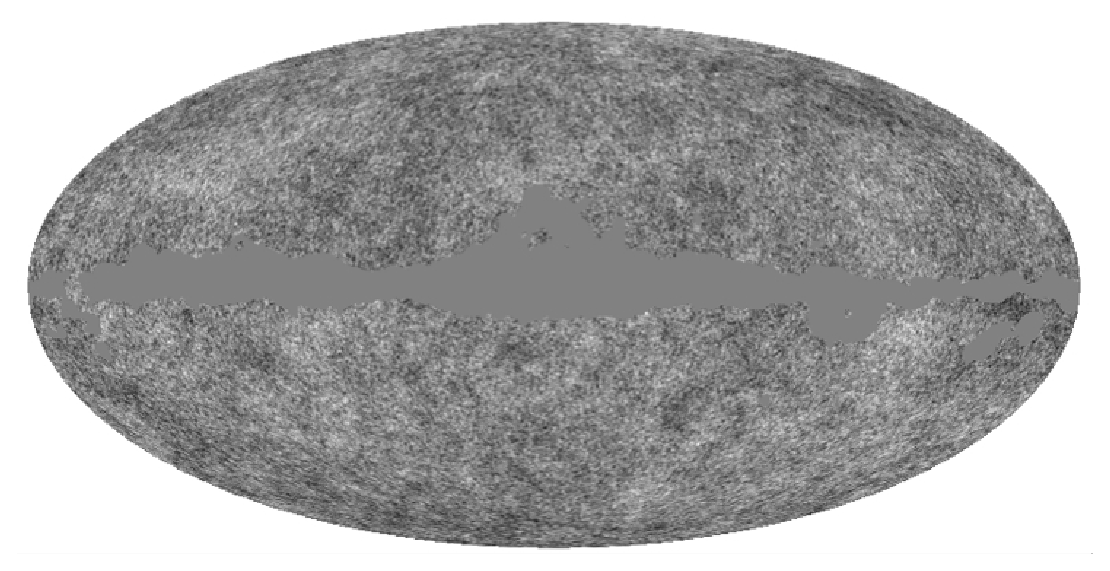
\includegraphics[width=7cm]{CMB_map}
% 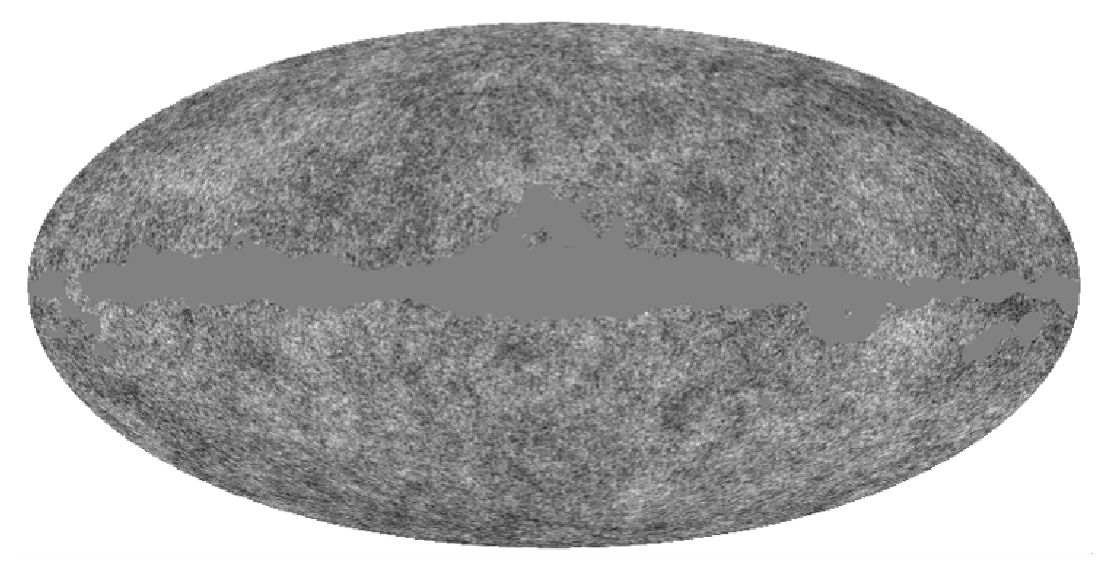
\includegraphics[width= 7cm]{CMB_w0db}
% 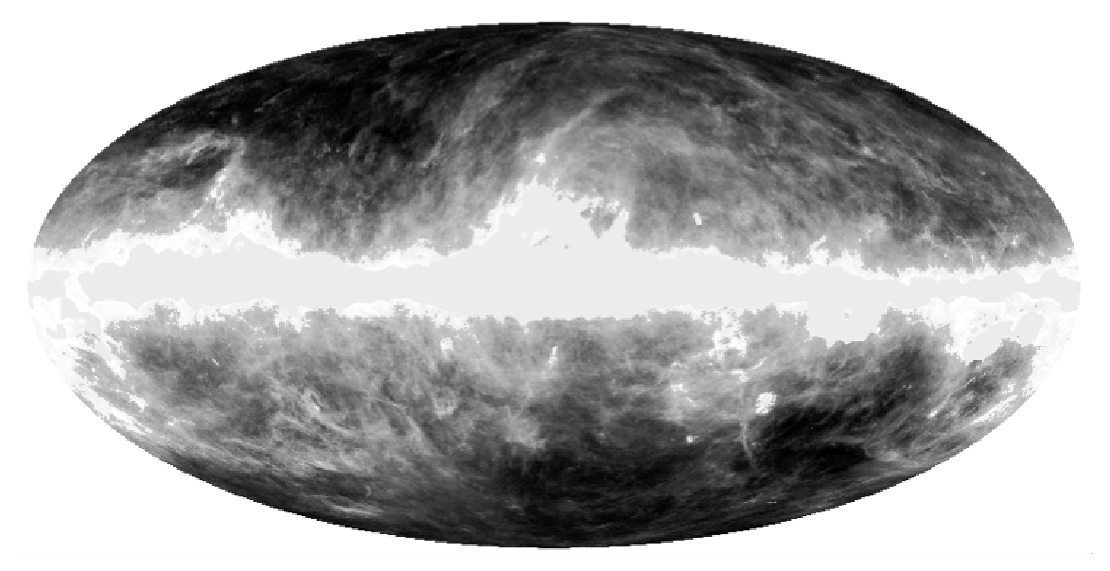
\includegraphics[width= 7cm]{hist_equal_dust}
% 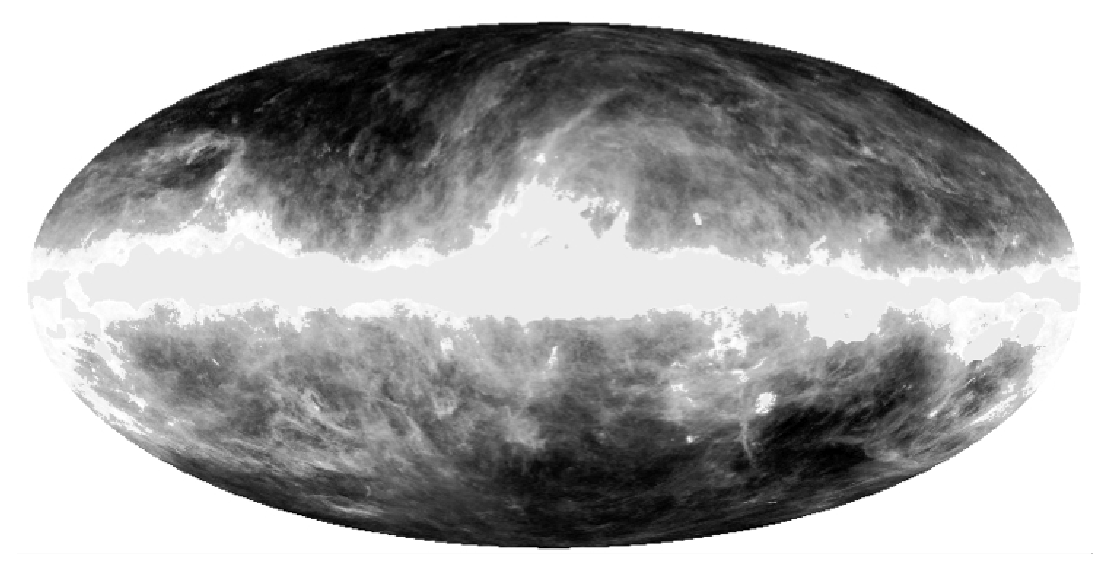
\includegraphics[width= 7cm]{hist_equal_dust_w_0db}
% 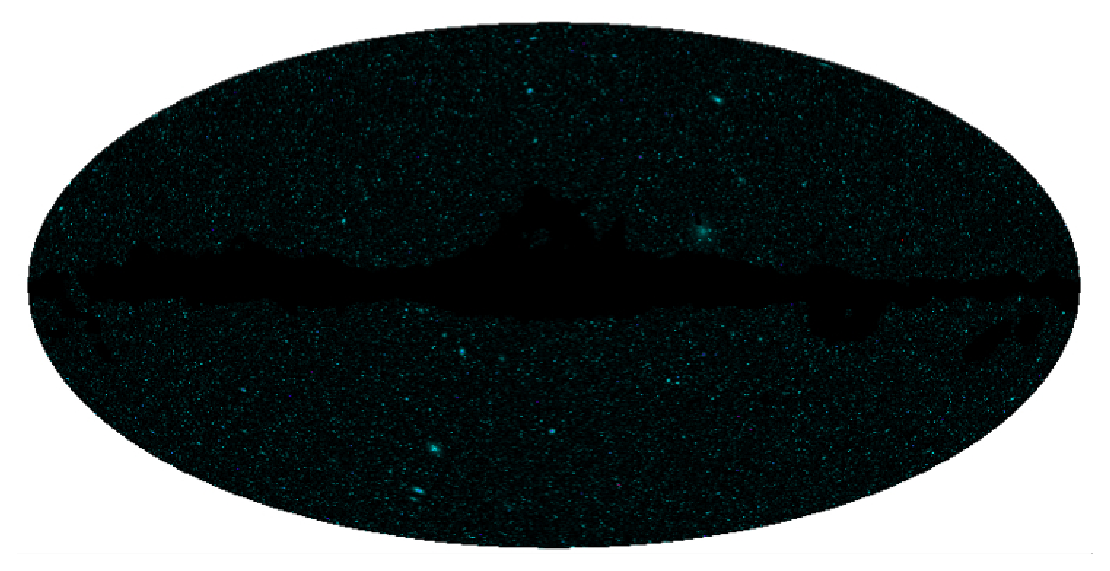
\includegraphics[width= 7cm]{sz_map3}
% 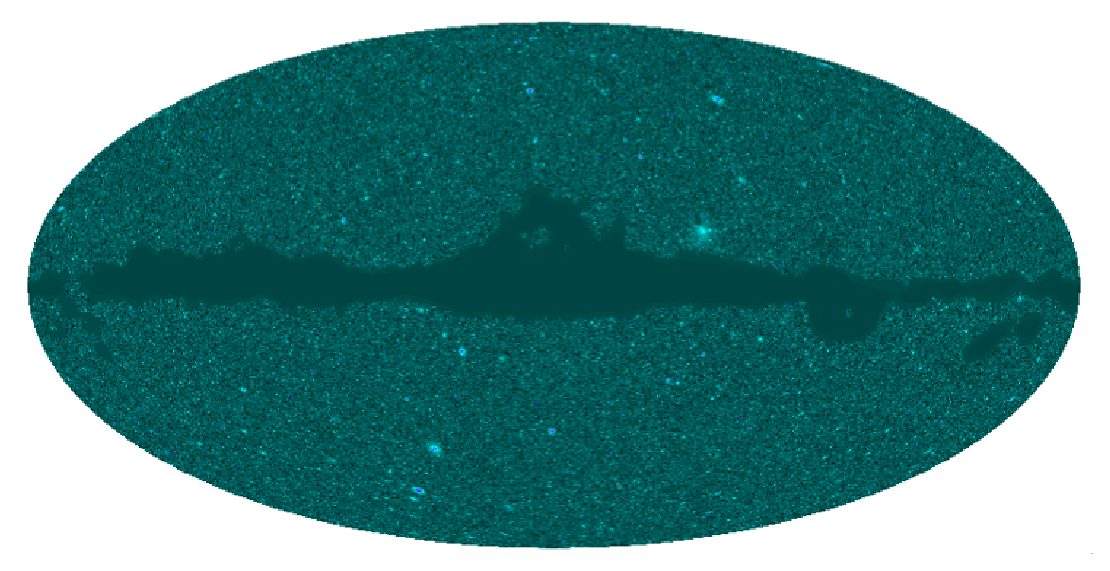
\includegraphics[width= 7cm]{sz_w_0db_bis}
% \caption{%%
% The maps on the left are the templates for CMB, galactic dust and SZ used in the experiment 
  % described in section~\ref{sec:NUMEXP}. The maps on the right were estimated using wSMICA 
  %  and scalewise Wiener filtering. (The different maps are drawn here in different color scales 
   % in order to enhance structures and ease visual comparisons).  } 
% \label{components}
% \end{center}
\vbox{
\centerline{
\hbox{
% \psfig{figure=CMB_w0db.ps,bbllx=0.5cm,bblly=7.5cm,bburx=21.5cm,bbury=20cm,width=7cm,clip=}
\psfig{figure=CMB_map.pdf,bbllx=0.5cm,bblly=7.5cm,bburx=21.5cm,bbury=20cm,width=7cm,clip=}
\psfig{figure=CMB_w0db.pdf,bbllx=0.5cm,bblly=7.5cm,bburx=21.5cm,bbury=20cm,width=7cm,clip=}
}}
\centerline{
\hbox{
\psfig{figure=hist_equal_dust.pdf,bbllx=0.5cm,bblly=7.5cm,bburx=21.5cm,bbury=20cm,width=7cm,clip=}
\psfig{figure=hist_equal_dust_w_0db.pdf,bbllx=0.5cm,bblly=7.5cm,bburx=21.5cm,bbury=20cm,width=7cm,clip=}
}}
\centerline{
\hbox{
\psfig{figure=sz_map3.pdf,bbllx=0.5cm,bblly=7.5cm,bburx=21.5cm,bbury=20cm,width=7cm,clip=}
\psfig{figure=sz_w_0db_bis.pdf,bbllx=0.5cm,bblly=7.5cm,bburx=21.5cm,bbury=20cm,width=7cm,clip=}
}}}
\caption{The maps on the left are zero mean templates for CMB ($\sigma =  4.17\times 10^{-5}$), galactic dust ($\sigma = 8.61\times 10^{-6}$) 
and SZ ($\sigma = 3.32\times 10^{-6}$) used in the experiment described in section~\ref{sect:NUMEXP}. The standard deviations given are for 
the region outside the galactic mask. The maps on the right were estimated using WSMICA and scalewise Wiener filtering as is explained in Appendix~2. 
Obviously, map reconstruction using Wiener filtering is optimal only in front of stationary Gaussian processes. For non Gaussian maps, such as 
given by the Sunyaev Zel'dovich effect, better reconstruction can be expected from non linear methods. The different maps are drawn here in 
different color scales in order to enhance structures and ease visual comparisons. }
\label{components}
\end{figure*}


\begin{figure}
\begin{center}
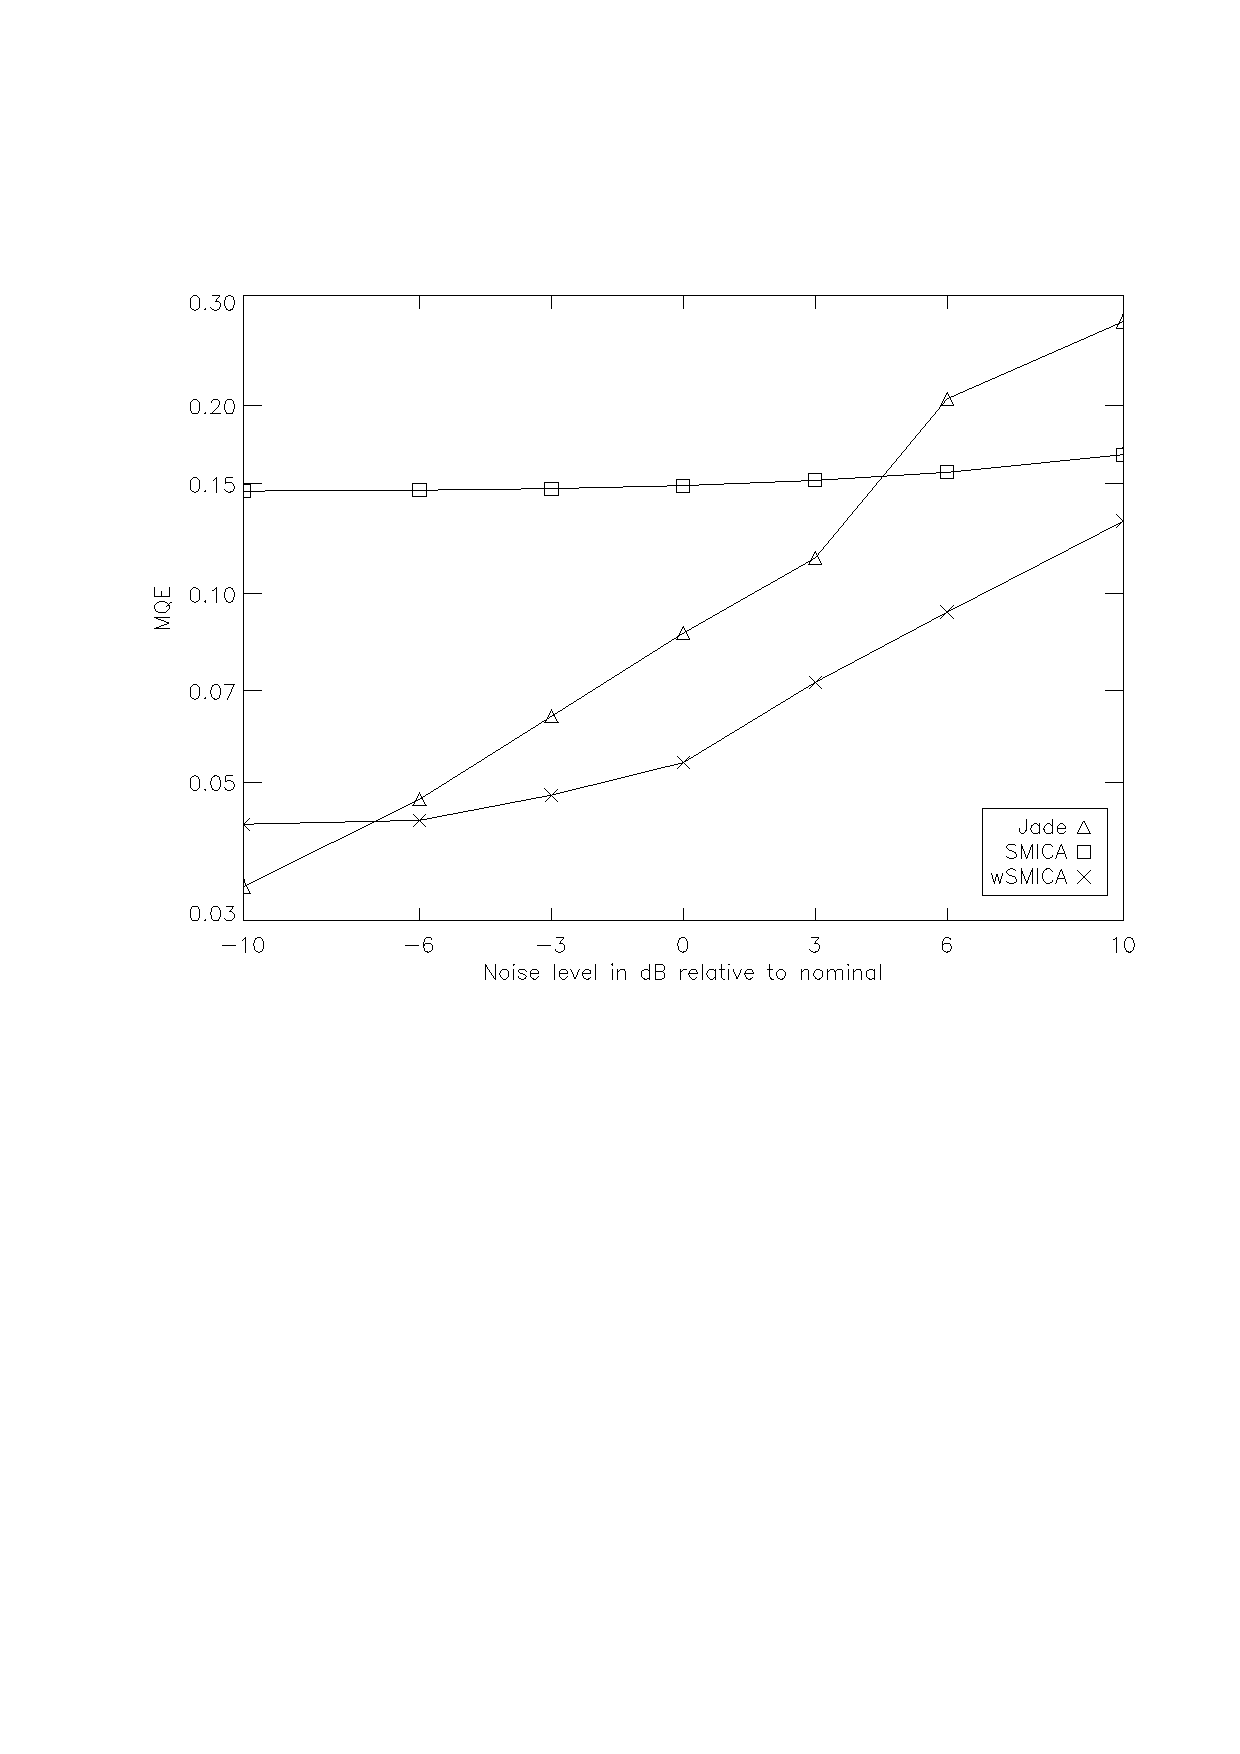
\includegraphics[width=8cm]{resultats_aa}
\caption{Relative reconstruction error defined by~(\ref{MQE}) of the CMB component map using SMICA, WSMICA and JADE as a function of the instrumental noise level in dB relative to the nominal values in table~\ref{NoiseScale}.} 
\label{resultats}
\end{center}
\end{figure}



\subsection{Sunyaev-Zeldovich cluster detection}

Another application of component separation techniques in astrophysics and cosmology is in the reconstruction of Sunyaev-Zel'dovich (SZ) 
galaxy clusters in future SZ-survey experiments such as Olimpo, APEX, or Planck which will use multiband bolometer cameras. The goal is 
to optimize SZ-Cluster extraction from the multichannel observed noisy maps. Resorting to blind methods is again attractive.

A complete description of the method we developed is given in~\cite{cluster:sz_cluster}. Before the actual detection of the SZ clusters, 
the multichannel data maps are combined and filtered to produce a clean map of the SZ component, with greater signal to noise ratio. We used 
an ICA approach to estimate the mixing matrix and perform the separation. A non linear filtering technique in the wavelet domain was used 
for the purpose of denoising. Finally a detection algorithm extracts the SZ clusters candidates from the restored SZ map. This is a new 
application of ICA to multichannel astrophysical data analysis. 

In the 100 to 600~GHz range, the brightest components of the sky are the Cosmic Microwave Background (CMB), the Infrared Point Sources, 
the Galactic dust emission and, swamped in the previous ones, the SZ clusters. It follows that the true sky map $X_{\nu}(\vartheta, \varphi)$, 
in a given optic band centered on $\nu$, can be modeled as a sum of distinct astrophysical radiations as in
\begin{equation} \label{SkyBandModel1}
	X_{\nu}(\vartheta, \varphi)  =  CMB_{\nu}(\vartheta, \varphi)  + IR_{\nu}(\vartheta, \varphi)  + Gal_{\nu}(\vartheta, \varphi)  + SZ_{\nu}(\vartheta, \varphi) 
\end{equation}
where $\vartheta, \varphi$ denote spatial or angular indexes on 2D or spherical maps. Assuming again that the radiative properties of the sources 
are completely isotropic in the sense that they do not depend on the direction of observation, the above model can be rewritten in the following factored form:
\begin{equation} \label{SkyBandModel2}
X_{\nu}(\vartheta, \varphi) =  \sum_{i} a_{\nu, i} S_{i}(\vartheta, \varphi)  \,\,+\,\, N_{\nu}(\vartheta, \varphi)
\end{equation}
where $S_{i}$ is the spatial template and $a_{\nu, i}$  the emission law of the $i\,{\textrm{th}}$ astrophysical component. Although this is 
a coarse approximation in the case of Infrared Point Sources, it is mostly valid for the other three components. With observations available 
in $m$ channels, assuming the beam varies only slightly as a function of $\nu$, equation~(\ref{SkyBandModel2}) can be written in matrix form : 
\begin{equation} \label{SkyBandModel3}
X(\vartheta, \varphi) = A\,\, S(\vartheta, \varphi)  \,\,+\,\, N(\vartheta, \varphi)
\end{equation}
where $X(\vartheta, \varphi)$ is a vector in $\mathbb{R}^m$, $A$ is an $m\times n$ matrix, n is the number of contributing astrophysical components, 
$S(\vartheta, \varphi)$ is now a vector in  $\mathbb{R}^n$ and $N(\vartheta, \varphi)$ in $\mathbb{R}^m$. Equation~(\ref{SkyBandModel3}) expresses 
that the observations consist of linear mixtures of astrophysical components with different weights and additive noise. 

Simulations of the major contributions in the frequency range considered here were generated according to the procedure described 
in~\cite{cluster:sz_cluster}. Figure~\ref{RawMaps} shows such typical simulations. These four physical components are linearly 
combined into a ``true" sky maps which are then convolved  with the experimental beam. Then instrumental noise is added. The resulting 
noisy mixture maps, as shown on figure~\ref{NoisyMaps} would be what the analysis team would recover from the data, after pointing 
reconstruction, outlier removal, de-correlation of instrumental systematics in the data, and map-making. 

\begin{figure*}[htp]
\vbox{
\centerline{
\hbox{
\psfig{figure=CMB.pdf,bbllx=3.cm,bblly=6.cm,bburx=19.1cm,bbury=21.7cm,height=7.5cm,width=6.5cm,clip=}
\hspace{0.2cm}
\psfig{figure=SZOld.pdf,bbllx=3.cm,bblly=6.cm,bburx=19.1cm,bbury=21.7cm,height=7.5cm,width=6.5cm,clip=}
}}
\vspace{0.3cm}
\centerline{
\hbox{
\psfig{figure=IR.pdf,bbllx=3.cm,bblly=6.cm,bburx=19.1cm,bbury=21.7cm,height=7.5cm,width=6.5cm,clip=}
\hspace{0.2cm}
\psfig{figure=TheGalax.pdf,bbllx=3.cm,bblly=6.cm,bburx=19.1cm,bbury=21.7cm,height=7.5cm,width=6.5cm,clip=}
}}
}
\caption{The 4 physical components of the sky included in our simulation: 
{\bf a)} is a map of the CMB's anisotropies in unit of $\mu$K, 
{\bf b)} is the SZ Cluster map, in unit of y Compton, 
{\bf c)} is the IR point source map, convolved with a beam of 2 arcmin, in Jy at 350GHz, finally 
{\bf d)} is the Galactic dust map in unit of MJy/st at 100 $\mu$m.}
\label{RawMaps}
\end{figure*}



%
%
%
\begin{figure*}[htp]
\vbox{
\centerline{
\hbox{
\psfig{figure=c143GHz.pdf,bbllx=3.cm,bblly=6.cm,bburx=19.1cm,bbury=21.7cm,height=7.0cm,width=6.0cm,clip=}
\hspace{0.2cm}
\psfig{figure=c217GHz.pdf,bbllx=3.cm,bblly=6.cm,bburx=19.1cm,bbury=21.7cm,height=7.0cm,width=6.0cm,clip=}
}}
\vspace{0.2cm}
\centerline{
\hbox{
\psfig{figure=c385GHz.pdf,bbllx=3.cm,bblly=6.cm,bburx=19.1cm,bbury=21.7cm,height=7.0cm,width=6.0cm,clip=}
\hspace{0.2cm}
\psfig{figure=c600GHz.pdf,bbllx=3.cm,bblly=6.cm,bburx=19.1cm,bbury=21.7cm,height=7.0cm,width=6.0cm,clip=}
}}
}
\caption{Simulated maps in Olimpo's four frequency bands. {\bf upper right} is the 147 GHz Band, {\bf upper left)} is the 217 GHz Band, {\bf lower right} is 
the 385 GHz Band: CMB anisotropies, IR point sources and Galactic Dust blend in this band {\bf lower left} 500 GHz: IR point sources and Galactic Dust are 
the dominant features at high frequencies. SZ cluster signal is dominated by other astrophysical sources at all frequencies.}
\label{NoisyMaps}
\end{figure*}
%
%
%



Any mainstream ICA algorithm for sparse sources, based on maximizing non-Gaussianity, would probably be successful at separating the SZ component map. 
We chose to use JADE in the wavelet domain, as described in section~\ref{sec:wjade}. Wavelets come into play as a sparsifying transform : data is sparse 
on a basis when this basis allows to describe that signal with a small number of coefficients. This is a highly desirable property, since noise is not 
expected to be sparse at the same time on such a basis. Choosing a sparsifying basis thus allows to enhance signal to noise ratio. Moving the data to 
a wavelet representation does not affect its information content and applying a wavelet transform on both sides of~(\ref{model0}) does not affect the 
mixing matrix and the model structure is preserved. However, the statistical distribution of the data coefficients in the new representation is different: 
wavelets are known to lead to sparse approximately \emph{i.i.d.} representations of structured data. Further, the \emph{local} (coefficient wise) signal 
to noise ratio depends on the choice of a representation. A wavelet transform tends to grab the informative coherence between pixels while averaging 
the noise contributions, thus enhancing structures in the data. Although the standard ICA model is for a noiseless setting, the derived methods can be 
applied to real data. Performance will depend on the detectability of significant coefficients \emph{i.e.} on the sparsity of the statistical distribution 
of the coefficients. Moving to a wavelet representation will then often lead to more robustness to noise. We noted that the estimation of the mixing matrix 
could be slightly enhanced by prefiltering the data using a Gaussian with the same width as the optical beam. The resulting SZ component map is shown 
on figure~\ref{JADEMaps}. Different filtering techniques were applied on this map and the results of a quantitative comparison are given in~\cite{cluster:sz_cluster}.




\begin{figure}[htp]
 \centerline{
\hbox{
%\psfig{figure=SZJadeG1_69w.ps}
\psfig{figure=SZJadeG1_69w.pdf,bbllx=3.cm,bblly=6.cm,bburx=19.1cm,bbury=21.8cm,height=6.5cm,width=6.5cm,clip=}
}
}
\caption{SZ component map extracted by JADE from the four observed noisy maps. The SZ cluster signal, subdominant at all observed frequencies, 
now appears clearly. No obvious leftovers from other astrophysical sources are seen. \textbf{Remaining noise is small, because we prefiltered 
data before JADE processing, and we simulated the nominal noise levels of an ambitious project: Olimpo.}}
\label{JADEMaps}
\end{figure}


 


% Deconvolution chapter

\chapter{Data Restoration on the Sphere}
\label{ch_restore}
\index{Denoising}
\index{Filtering}

\label{sect_exp}
\section{Introduction}
\index{wavelet!denoising}
\index{curvelet!denoising}

Wavelets and Curvelets have been used successfully for image denoising \emph{via} non-linear filtering or 
thresholding methods \cite{starck:book02,starck:sta01_3}. Hard thresholding, for instance, consists in 
setting all insignificant coefficients (\emph{i.e.} coefficients with an absolute value below a given 
threshold) to zero. In practice, we need to estimate the noise standard deviation $\sigma_j$ in each band 
$j$ and a wavelet (or curvelet) coefficient $w_j$ is significant if $\mid w_j \mid > k \sigma_j$, where $k$ 
is a user-defined parameter, typically chosen between 3 and 5. The $\sigma_j$ estimation in band $j$ can be 
derived from simulations \cite{starck:book02}. Denoting $D$ the noisy data and $\delta$ the thresholding 
operator, the filtered data $\tilde D$ are obtained by : 
\begin{eqnarray}
 {\tilde D} =    {\cal R} \delta( {\cal T} D)
\end{eqnarray}
where ${\cal T}$ is the wavelet (resp. curvelet) transform operator and ${\cal R}$ is the wavelet (resp. curvelet) reconstruction operator. 


\section{Significant Wavelet Coefficients}
\label{ch_noise}
\subsection{Definition}
\index{noise}
\index{wavelet!significant coefficient}

In most applications, it is necessary to know if a wavelet coefficient is due to signal (i.e.\ it is significant) or to noise. 

The wavelet (resp. curvelet) transform yields a set of resolution-related views of the input image. 
A wavelet (resp. curvelet) band at level $j$ has coefficients given by $w_{j,k}$. If we obtain the 
distribution of the coefficient $w_{j,k}$ for each band of the decomposition, based on the noise, 
we can introduce a statistical significance test for this coefficient. This procedure is the classical 
significance-testing one. Let ${\cal H}_0$ be the hypothesis that the image is locally constant at scale $j$.  
Rejection of hypothesis ${\cal H}_0$ depends (for positive coefficient values) on:
\begin{eqnarray}
P = Prob(\mid w_{j,k} \mid \ < \ \tau \mid {\cal H}_0)  
\end{eqnarray}
The detection threshold, $\tau$, is defined for each scale. Given an estimation threshold, $\epsilon$, 
if $P = P(\tau) > \epsilon$ the null hypothesis is not excluded. Although non-null, the value of the 
coefficient could be due to noise. On the other hand, if $P < \epsilon$, the coefficient value cannot be due to 
the noise alone, and so the null hypothesis is rejected. In this case, a significant coefficient has been detected.

\subsection{Noise Modeling}
\index{noise}
\index{noise!Gaussian}
If the distribution of $w_{j,l}$ is Gaussian, with zero mean and standard deviation $\sigma_j$, we have the probability density
\begin{eqnarray}
p(w_{j,l}) = \frac{1}{\sqrt{2\pi} \sigma_j} e^{{- w_{j,l}^2}/2\sigma^2_j} 
\end{eqnarray}
Rejection of hypothesis ${\cal H}_0$ depends (for a positive coefficient value) on:
\begin{eqnarray}
P = Prob( w_{j,l} > W) = \frac{1}{\sqrt{2\pi} \sigma_j} \int^{+\infty}_{w_{j,l}} e^{-W^2/2\sigma^2_j} dW 
\end{eqnarray}
and if the coefficient value is negative, it depends on 
\begin{eqnarray}
P = Prob( w_{j,l} < W) = \frac{1}{\sqrt{2\pi} \sigma_j} \int^{w_{j,l}}_{-\infty} e^{-W^2/2\sigma^2_j} dW 
\end{eqnarray}

Given stationary Gaussian noise, it suffices to compare $w_{j,l}$ to 
\index{stationary signal}
$k \sigma_j$.  Often $k $ is chosen as 3, which corresponds approximately to $\epsilon = 0.002$.  
If $w_{j,l}$ is small, it is not significant and could be due to noise. If $w_{j,l}$ is large, it is significant:
\begin{eqnarray}
\begin{array}{l}
\mbox{ if }  \mid  w_{j,l} \mid \ \geq \ k \sigma_j \ \ \mbox{ then } w_{j,l}   \mbox{ is significant } \\ 
\mbox{ if }  \mid  w_{j,l} \mid \ < \ k \sigma_j \ \ \mbox{ then }  w_{j,l} \mbox{ is not significant }
\end{array}
\end{eqnarray}

So we need to estimate, in the case of Gaussian noise models, the noise standard deviation at each scale. 
These standard deviations can be determined analytically, but the calculations can become complicated.  

The appropriate value of $\sigma_j$ in the succession of wavelet planes is assessed from the standard deviation 
of the noise $\sigma_N$ in the original data $D$, and from study of the noise in the wavelet space. This study 
consists of simulating a data set containing Gaussian noise with a standard deviation equal to 1, and taking the 
wavelet transform of this data set. Then we compute the standard deviation $\sigma^e_j$ at each scale. We get a curve 
$\sigma^e_j$ as a function of $j$, giving the behavior of the noise in the wavelet space (Note that if we had used 
an orthogonal wavelet transform, this curve would be linear). Due to the properties of the wavelet (resp. curvelet) 
transform, we have $ \sigma_j = \sigma_N \sigma^e_j $. The noise standard deviation at scale $j$ of the data is equal 
to the noise standard deviation $\sigma_N$ multiplied by the noise standard deviation at scale $j$ of the simulated data.

\subsection{Automatic Estimation of Gaussian Noise}
\subsubsection{$k$-sigma clipping}
\index{sigma clipping}
\index{noise!sigma clipping}
\index{noise}
The Gaussian noise $\sigma_N$ can be estimated automatically in a data set $D$. This estimation is particularly important, 
because all the noise standard deviations $\sigma_j$ in the scales $j$ are derived from $\sigma_N$. Thus an error associated 
with $\sigma_N$ will introduce an error on all $\sigma_j$. Noise is therefore more usefully estimated in the high frequencies, 
where it dominates the signal. The resulting method consists first of filtering the data $D$ with an average filter or the 
median filter and subtracting from $D$ the filtered signal $F$: $S = D - F $. In our case, we replace $S$ by the first scale 
of the wavelet transform ($S = w_1$), which is more convenient from the computation time point of view. The histogram of $S$ 
shows a Gaussian peak around 0. A k-sigma clipping is then used to reject pixels where the signal is significantly large. 
We denote $S^{(1)}$ the subset of $S$ which contains only the pixels such that $\mid S_l \mid \ < k \sigma_S$, where $\sigma_S$ 
is the standard deviation of $S$, and $k$ is a constant generally chosen equal to 3. By iterating, we obtain the subset $S^{(n+1)}$ 
verifying $\mid S^{(n)}_l \mid \ < k \sigma_{S^{(n)}}$, where $\sigma_{S^{(n)}}$ is the noise standard deviation of $S^{(n)}$. 
Robust estimation of the noise $\sigma_1$ in $w_1$ (as $S = w_1$) is now obtained by calculation of the standard deviation of 
$S^{(n)}$ ($\sigma_1 = \sigma_{S^{(n)}}$). In practice, three iterations are enough, and accuracy is generally better than $5$\%.
$\sigma_N$ is finally calculated by: 
\be
\sigma_N = \frac{\sigma_1}{\sigma^e_1} = \frac{\sigma_{S^{(n)}} }{\sigma^e_1}
\ee


\subsection{Correlated Noise}
\index{median!median absolute deviation}
\index{MAD}
\index{noise!median absolute deviation}
\index{noise}
In this case, the data can be treated as for the Gaussian case, but the noise standard deviation $\sigma_j$ at scale $j$ 
is calculated independently at each scale. Two methods can be used: 
\begin{enumerate}
\item $\sigma_j$ can be derived from a k-sigma clipping method applied at scale $j$.
\item The median absolute deviation, MAD, can be used as an estimator of the noise standard deviation:
\begin{eqnarray}
\sigma_j = \mbox{median}( \mid w_j \mid ) / 0.6745
\end{eqnarray}
\end{enumerate}

\section{Thresholding}
Many filtering methods have been proposed in the last ten years. {\em Hard thresholding} consists of setting to 0 all 
wavelet coefficients which have an absolute value lower than a threshold $T_j$ (non-significant wavelet coefficient):
\begin{eqnarray}  \tilde w_{j,k} = 
\left\{ \begin{array}{ll} w_{j,k} &  \mbox{ if } \mid w_{j,k} \mid \geq T_j  \nonumber  \\ 

0 &  \mbox{ otherwise}  \end{array} \right. 
\end{eqnarray}
where $w_{j,k}$ is a wavelet coefficient at scale $j$ and at spatial position $k$. 

{\em Soft thresholding} consists of replacing each wavelet coefficient by the value $\tilde w$ where
\begin{eqnarray}  \tilde w_{j,k} = 
\left\{ \begin{array}{ll} sgn(w_{j,k}) ( \mid w_{j,k} \mid - T_j)    &  \mbox{ if } \mid w_{j,k} \mid \geq T_j \nonumber  \\ 
0 &  \mbox{ otherwise}  \end{array} \right. 
\end{eqnarray} 
This operation is generally written as:
\begin{eqnarray} 
 \tilde w_{j,k} = \mathrm{soft}( w_{j,k})  = sgn(w_{j,k}) ( \mid w_{j,k} \mid - T_j)_{+}
\end{eqnarray} 
where $(x)_{+} = MAX(0,x)$.

When the discrete orthogonal wavelet transform is used instead of the \`a trous algorithm, it is interesting to note
that the hard and soft thresholded estimators are solutions of the following minimization problems:
\begin{eqnarray*}
  \tilde w  =   \mathrm{arg}_w \min {1 \over 2} \parallel D - {\cal W}^{-1} w \parallel^2_{l^2} + 
 \lambda \parallel w \parallel^2_{l^0} & & \mbox{\bf   hard threshold} \nonumber \\
  \tilde w   =   \mathrm{arg}_w \min {1 \over 2} \parallel D - {\cal W}^{-1} w \parallel^2_{l^2} + 
 \lambda \parallel w \parallel^2_{l^1} & & \mbox{\bf   soft threshold}  
\end{eqnarray*}
where $D$ is the input data, ${\cal W}$ the wavelet transform operator, and $l^0$ indicates the limit of $l^\delta$ 
when $\delta \rightarrow 0$. This counts in fact the number of non-zero elements in the sequence.
\index{thresholding!hard}
\index{thresholding!soft}
\index{wavelet!hard threshold}
\index{wavelet!soft threshold}

As described before, in the case of Gaussian noise, $T_j = K \sigma_j$, where $j$ is the scale of the wavelet coefficient, 
$\sigma_j$ is the noise standard deviation at the scale $j$, and $K$ is a constant generally chosen equal to 3.

Other threshold methods have been proposed, like the {\em universal threshold} 
\index{universal threshold}
\index{SURE}
\index{thresholding!universal threshold}
\index{thresholding!SURE}
\cite{rest:donoho93_1,rest:donoho93_2}, or the SURE (Stein Unbiased Risk Estimate) method \cite{rest:donoho95},
but they generally do not yield as good results as the hard thresholding method based on the significant coefficients.  
For astronomical data, soft thresholding should never be used because it leads to a photometry loss associated with all 
objects, which can easily be verified by looking at the residual map (i.e.\ data $-$ filtered data). Concerning the 
threshold level, the universal threshold  corresponds to a minimum risk. The larger the number of pixels, the larger 
is the risk, and it is normal that the threshold $T$ depends on the number of pixels ($T = \sqrt{2\log n} \sigma_j$, 
$n$ being the number of pixels). The $K\sigma$ threshold corresponds to a false detection probability, the probability 
to detect a coefficient as significant when it is due to the noise. The $3\sigma$ value corresponds to 0.27 \% false detection.
 
\begin{figure*}
% 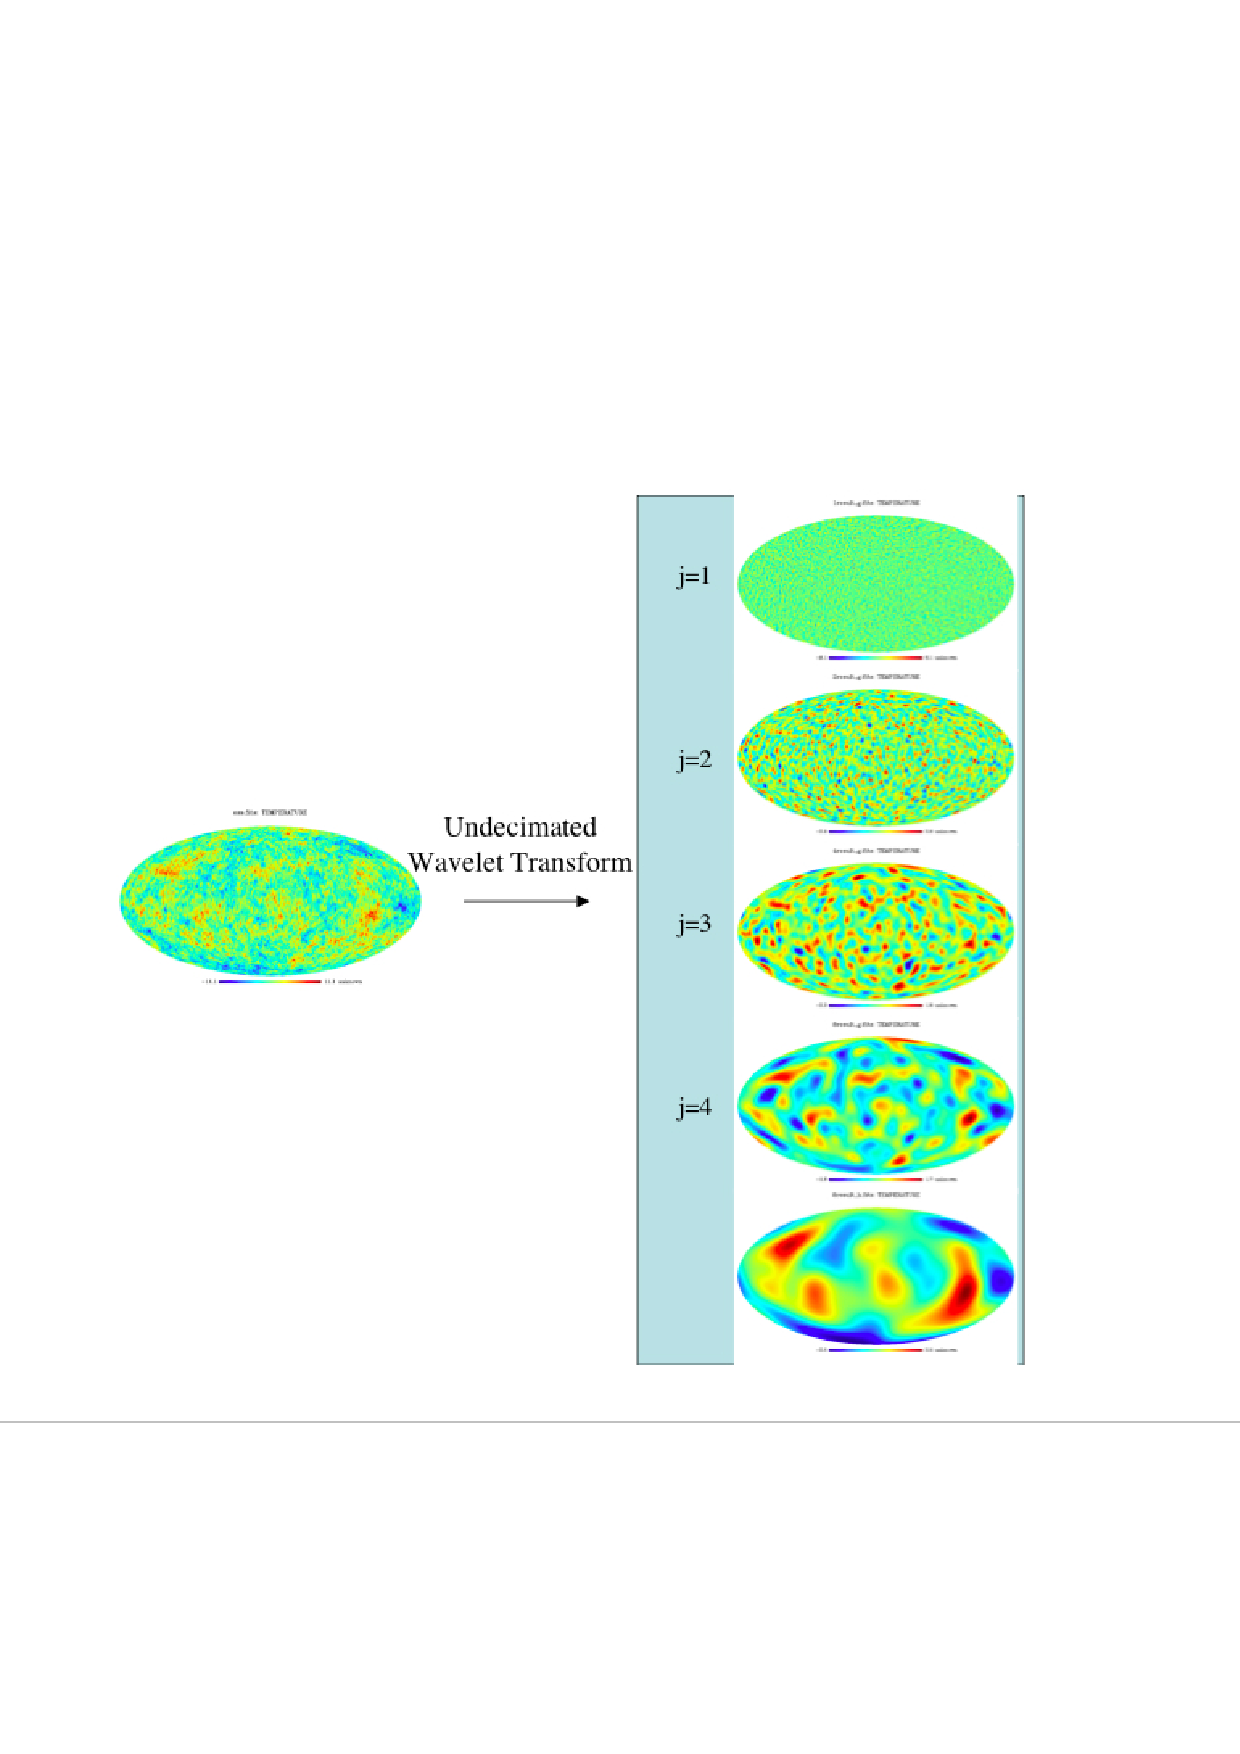
\includegraphics[height=8truecm,width=6truecm]{fig_uwt_sphere.pdf}
% 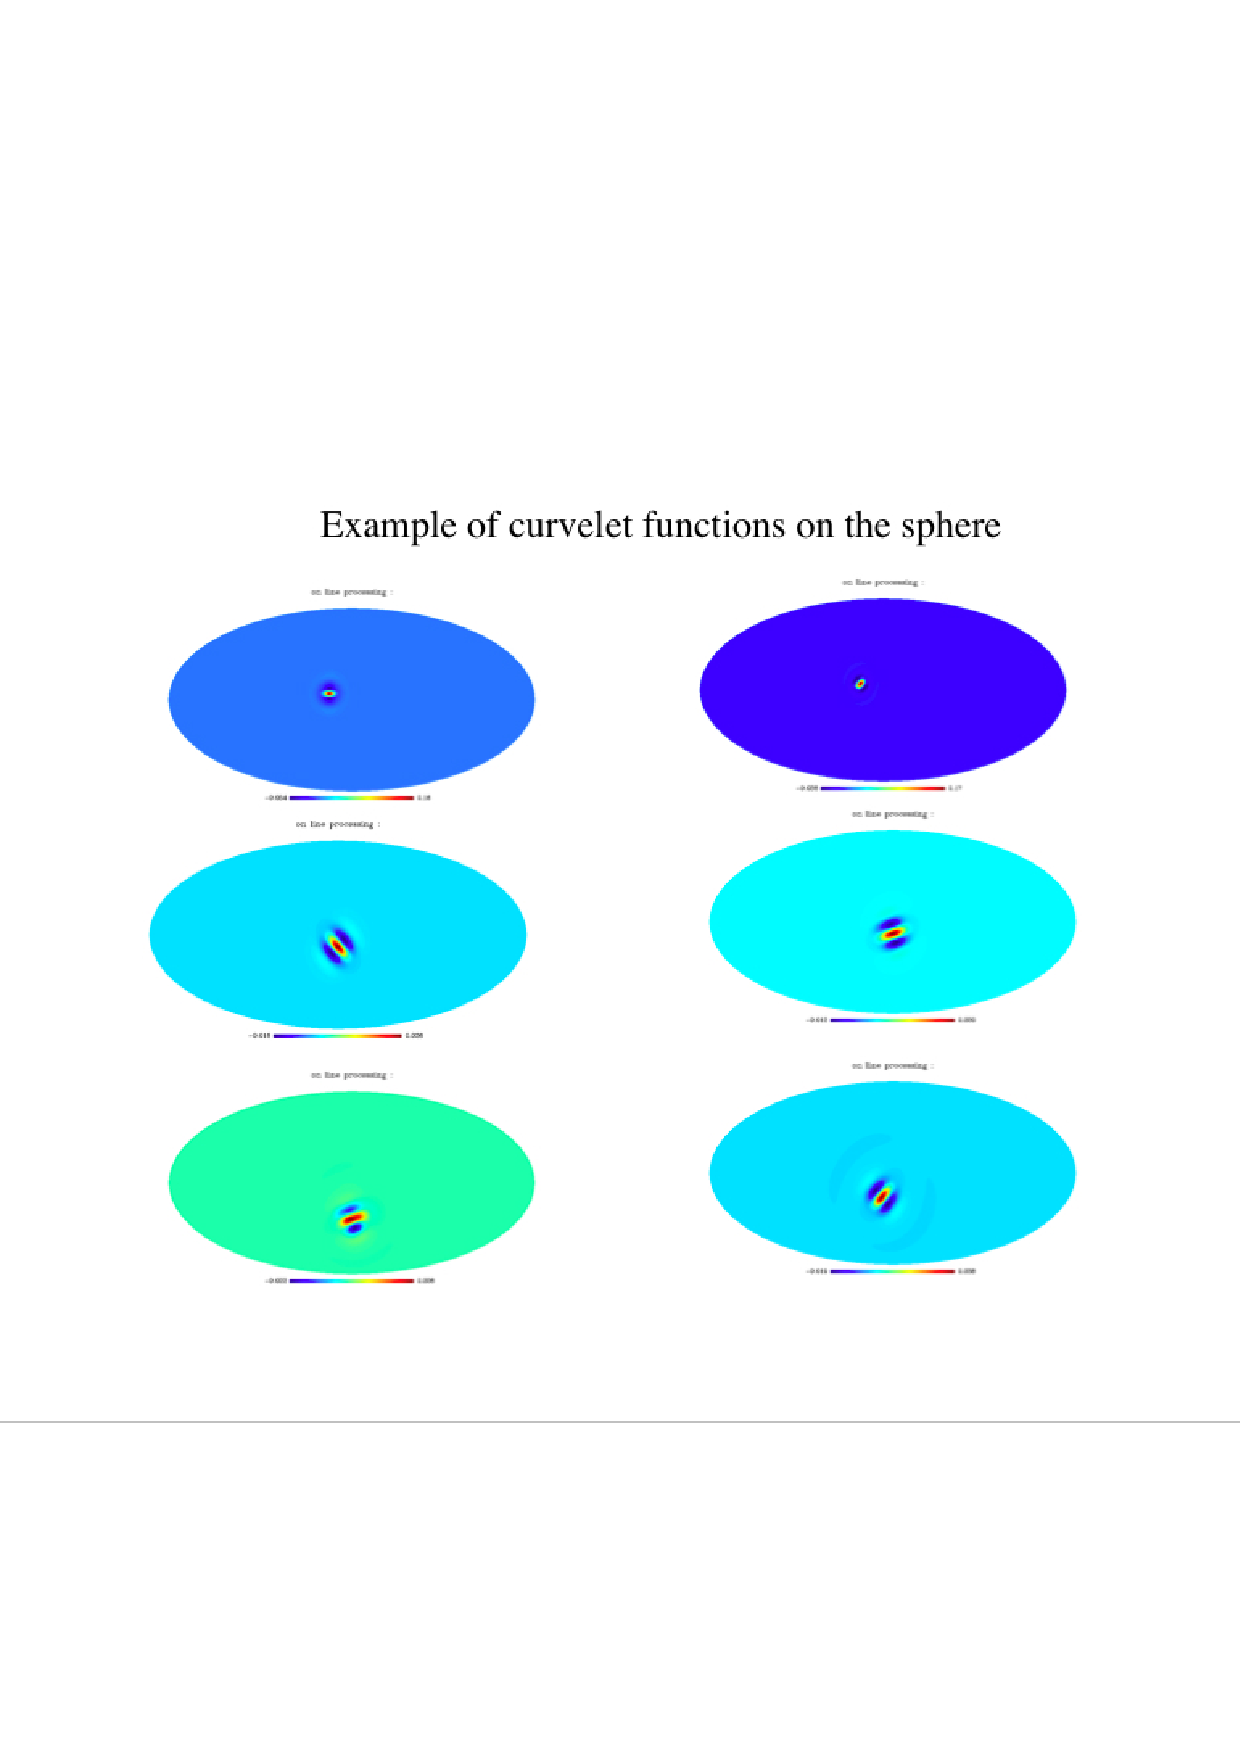
\includegraphics[height = 5 in]{fig_back_cur_sphere.pdf}
\vbox{
\centerline{
\hbox{
\psfig{figure=fig_synchrotron_bw.pdf,bbllx=0.5cm,bblly=9.5cm,bburx=20cm,bbury=20cm,width=8cm,height=4.5cm,clip=}
\psfig{figure=fig_synchrotron_noise5_bw.pdf,bbllx=0.5cm,bblly=9.5cm,bburx=20cm,bbury=20cm,width=8cm,height=4.5cm,clip=}
}}
\centerline{
\hbox{
\psfig{figure=fig_pwt5_synchrotron_noise5_bw.pdf,bbllx=0.5cm,bblly=9.5cm,bburx=20cm,bbury=20cm,width=8cm,height=4.5cm,clip=}
\psfig{figure=fig_resi_pwt5_synchrotron_noise5_bw.pdf,bbllx=0.5cm,bblly=9.5cm,bburx=20cm,bbury=20cm,width=8cm,height=4.5cm,clip=}
}}
\centerline{
\hbox{
\psfig{figure=fig_pcur5_synchrotron_noise5_bw.pdf,bbllx=0.5cm,bblly=9.5cm,bburx=20cm,bbury=20cm,width=8cm,height=4.5cm,clip=}
\psfig{figure=fig_resi_pcur5_synchrotron_noise5_bw.pdf,bbllx=0.5cm,bblly=9.5cm,bburx=20cm,bbury=20cm,width=8cm,height=4.5cm,clip=}
}}
}
\caption{\textbf{Denoising.} Upper left and right : simulated synchrotron image and same image with an additive 
Gaussian noise (\emph{i.e.} simulated data). Middle: pyramidal wavelet filtering and residual. Bottom: pyramidal 
curvelet filtering and residual.{ On such data, presenting very anisotropic features, the residual with a curvelet 
denoising is cleaner than with the wavelet denoising.}}
\label{Figure:sync_filter}
\end{figure*}

Figure~\ref{Figure:sync_filter} describes the setting and the results of a simulated denoising experiment : 
upper left, the original simulated map of the synchrotron emission (renormalized between 0 and 255); upper right, 
the same image plus additive Gaussian noise ($\sigma=5$); middle, the pyramidal wavelet filtered image and the 
residual (i.e. noisy data minus filtered data); bottom, the pyramidal curvelet transform filtered image and the 
residual. A $5 \sigma_j$ detection threshold was used in both cases. On such data, presenting very anisotropic 
features, the curvelets produces better results than the wavelets.


\section{The Combined Filtering Method on the Sphere}
\index{wavelet!combined filtering}
\index{curvelet!combined filtering}
\index{combined filtering method}

%\voffset -1truecm
{\small
\begin{table*}[htb]
\baselineskip=0.4cm
\begin{center}
\begin{tabular}{lccccc} \hline \hline
Method                          &  Error Standard Deviation     &  SNR (dB)    \\ \hline \hline
Noisy map                       & 5.  &      13.65  \\
Wavelet                         & 1.30  &    25.29  \\
Curvelet                        & 1.01  &    27.60  \\
CFM                             & 0.86  &    28.99  \\ \hline
\hline
\end{tabular}
\caption{Table of error standard deviations and SNR values after filtering the synchrotron noisy map (Gaussian white noise - sigma = 5 ) 
by the wavelet, the curvelet and the combined filtering method. Images are available at "http://jstarck.free.fr/mrs.html".}
% \vspace{0.5cm}aa_sphere05
\label{comptab_sync}
\end{center}
\end{table*}
}

\begin{figure}
% 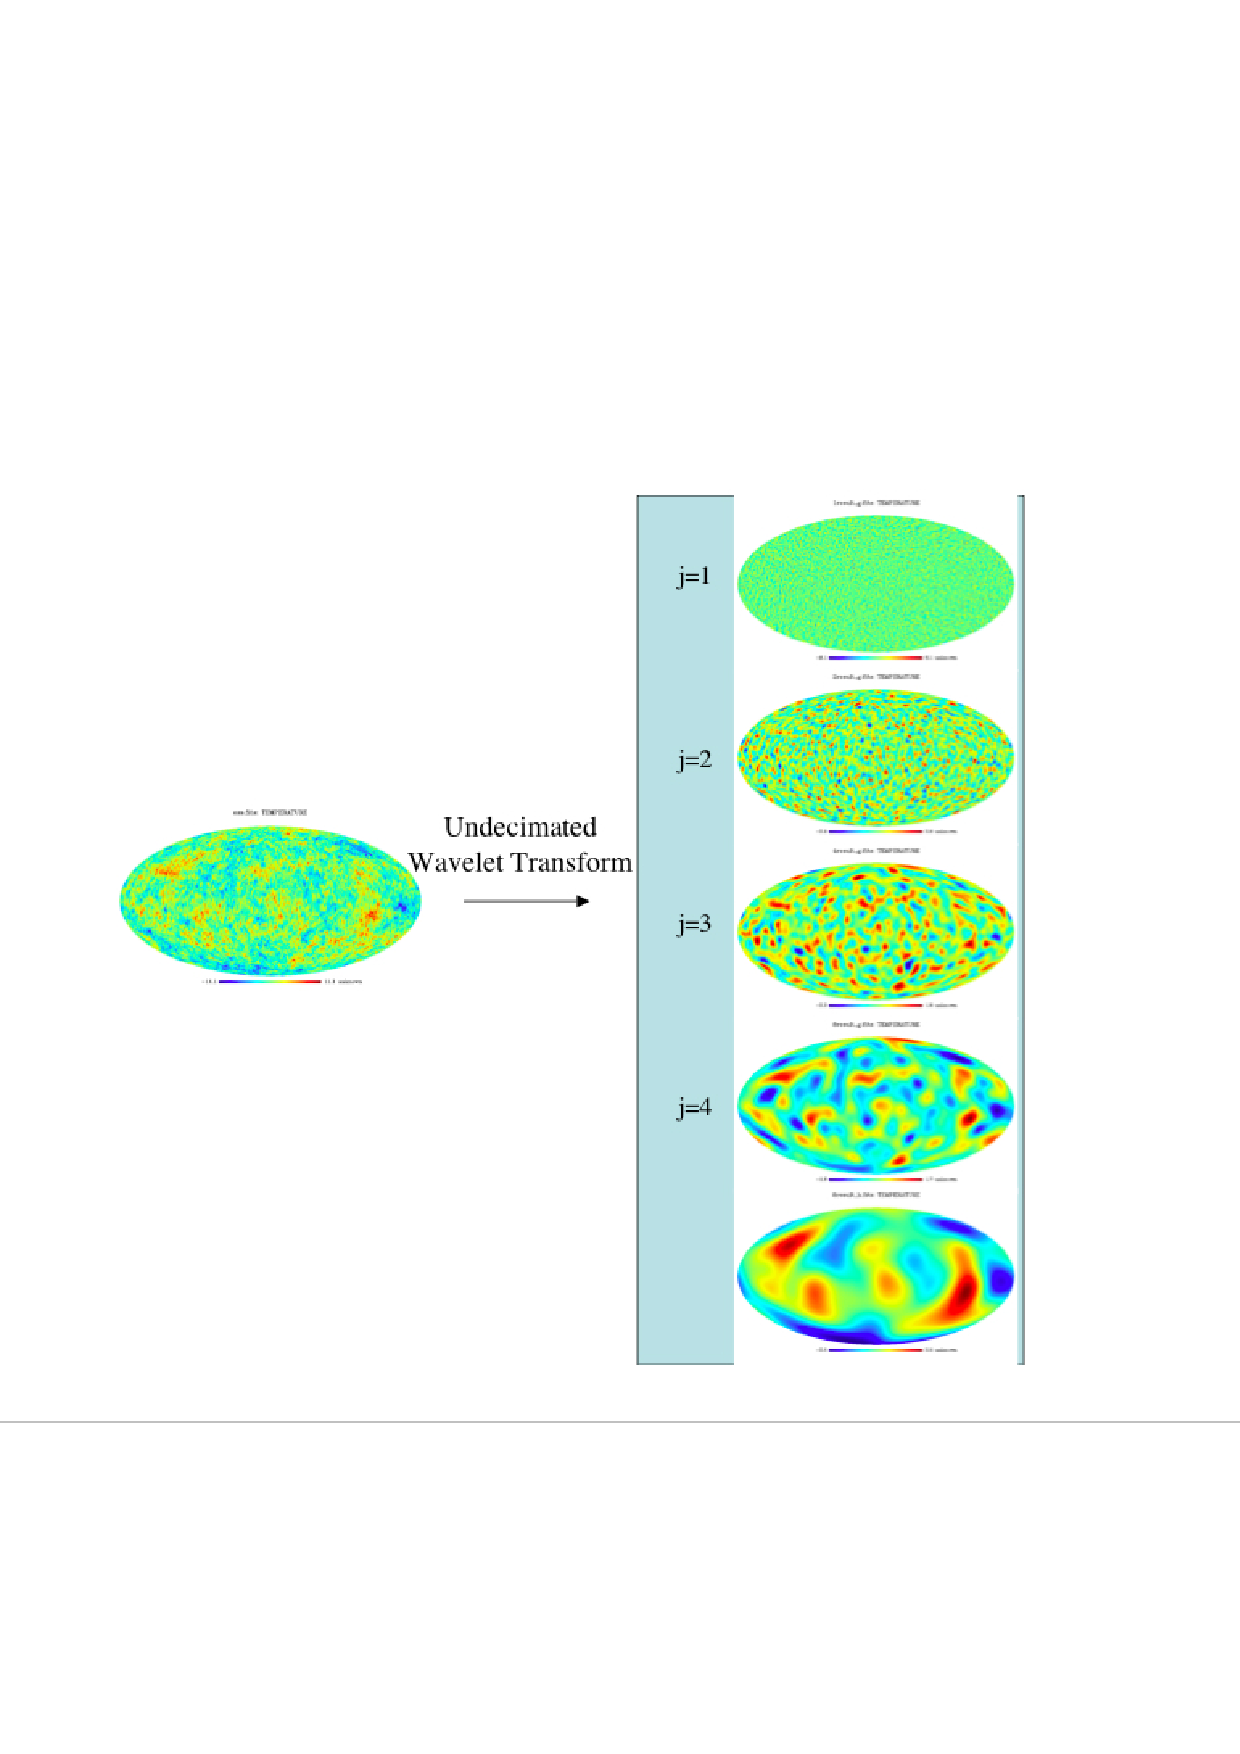
\includegraphics[height=8truecm,width=6truecm]{fig_uwt_sphere.pdf}
% 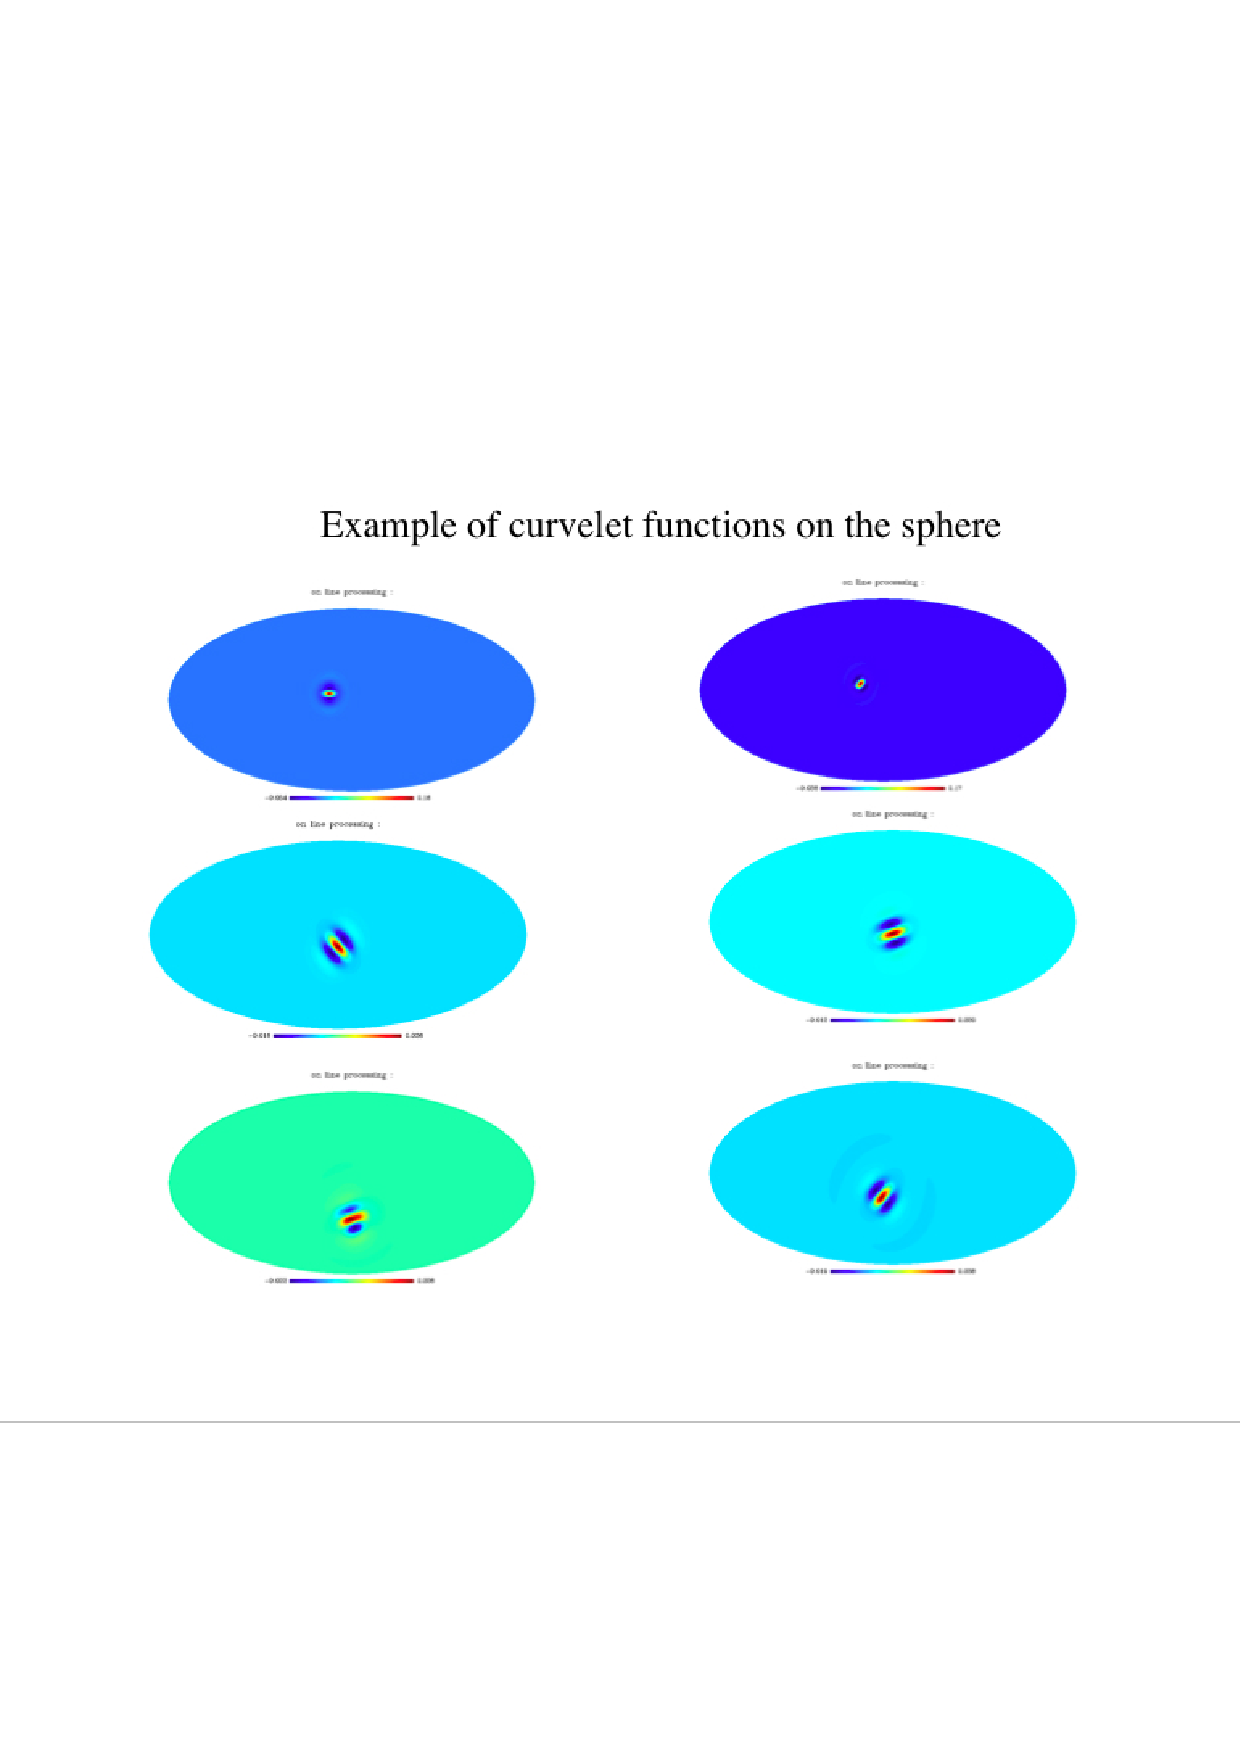
\includegraphics[height = 5 in]{fig_back_cur_sphere.pdf}
\centerline{
\hbox{
\psfig{figure=fig_cbf5_synchrotron_bw.pdf,bbllx=0.5cm,bblly=9.5cm,bburx=20cm,bbury=20cm,width=8cm,height=4.5cm,clip=}
\psfig{figure=fig_resi_cbf5_synchrotron_bw.pdf,bbllx=0.5cm,bblly=9.5cm,bburx=20cm,bbury=20cm,width=8cm,height=4.5cm,clip=}
}}
\caption{Denoising. Combined Filtering Method (pyramidal wavelet and pyramidal curvelet) and residual.}
\label{Figure:sync_cbf_filter}
\end{figure}


\begin{figure}
\centerline{
\hbox{
% \psfig{figure=fig_result_cbf_face5_bw.ps,bbllx=1.5cm,bblly=4.5cm,bburx=20cm,bbury=23cm,height=10cm,width=10cm,clip=}
\psfig{figure=fig_cmp_fil_synchrotron_face6_bw.pdf,bbllx=1.5cm,bblly=12.5cm,bburx=10.5cm,bbury=25.5cm,height=19.5cm,width=13.5cm,clip=}
}}
\caption{{ Combined Filtering Method, face 6 in the Healpix representation of the image shown in figure~\ref{Figure:sync_cbf_filter}. 
From top to bottom and left to right, respectively the a) original image face, b) the noisy image, c) the combined filtered image, 
d) the combined filtering residual, e) the wavelet filtering residual and f) the curvelet filtering residual.}}
\label{Figure:sync_face_cbf_filter}
\end{figure}

Although the results obtained by simply thresholding the curvelet expansion are encouraging, there is of course ample room for further
improvement. A quick inspection of the residual images for both the wavelet and curvelet transforms shown in Figure~\ref{Figure:sync_filter}
reveals the existence of very different features. For instance, wavelets do not restore long features with high fidelity while curvelets
are seriously challenged by isotropic or small features. Each transform has its own area of expertise and this complementarity is of great 
potential. The Combined Filtering Method (CFM) \cite{starck:spie01a} allows us to benefit from the advantages of both transforms. This iterative 
method detects the significant coefficients in both the wavelet domain and the curvelet domain and guarantees that the reconstructed map will 
take into account any pattern which is detected as significant by either of the transforms. A full description of the algorithm is given in Appendix B.
Figure~\ref{Figure:sync_cbf_filter} shows the CFM denoised image and its residual. { Figure~\ref{Figure:sync_face_cbf_filter} shows one face 
(face 6) of the following Healpix images: upper left, original image; upper right, noisy image; middle left, restored image after denoising 
by the combined transform; middle right, the residual; bottom left and right, the residual using respectively the curvelet and the wavelet 
denoising method. } The results are reported in Table~\ref{comptab_sync}. The residual is much better when the combined filtering is applied, 
and no feature can be detected any more by eye in the residual. This was not the case for either the wavelet and the curvelet filtering.

% \section{Deconvolution ?}


\chapter{Statistics on the Sphere and Non-Gaussianities Detection}

\section{Introduction}

\section{Kurtosis, HC from Wavelet and Curvelet Coefficients}

\section{The Multiscale Genus}

\section{Experiments}


% \section{Mutual Information}
\newpage
\chapter{Conclusion}
 
\clearpage
\newpage



\chapter{IDL Routines}
\label{ch_mrs_idl}
%\chapterhead{IDL Routines}
\markright{IDL Routines}


\section{Introduction}
A set of routines has been developed in IDL. Starting IDL using the script program {\em mrs.pro} allows the user 
to get the multiresolution environment on the sphere, and all routines described in the following can be called. 
An online help facility is also available by invoking the {\em mrsh} program under IDL.


\section{Installation}
\index{installation}

The MRS package requires that IDL (version 6.0 or later) and HEALPix (version 2.0) be installed. The HEALPix environment 
variable \textbf{HEALPix} is expected to be defined. The alias \textbf{idl} should also be defined to launch the IDL environment. 
Then, installing the MRS package simply requires adding some lines in your shell environment profile:
\begin{itemize}
\item[$\bullet$] {define the environment variable \textbf{MRS}}  
\begin{verbatim}
setenv MRS /home/user/mrs_1.0
\end{verbatim}
 \item[$\bullet$]{define the alias \textbf{mrs}}  
\begin{verbatim}
alias mrs 'idl $MRS/idl/mrs.pro' 
\end{verbatim}
\end{itemize}
Then the command "mrs" will start the IDL session using the MRS environment. Test program examples can be found 
in \$MRS/idl (test\_mrs.pro, test\_mrs\_smica.pro, \dots). These routines use data in directory \$MRS/data.


\section{General functions for spherical maps}
\index{general}

\subsection{Reading a spherical map from a file : mrs\_read}
\index{IDL routines!mrs\_read}
\index{general!read map}
Read a spherical map, either in HEALPIX or in GLESP format.
{\bf
\begin{center}
     USAGE: map = mrs\_read( file )
\end{center}}
where
\begin{itemize}
\item {\em file} : Input string, name of the file to be read. The pathname can be included in the string, by default 'file.fits' is equivalemt to './file.fits'
\item {\em map} : Output IDL array of Healpix map or Glesp image IDL structure, map read. For a Healpix map, the map is setted to the NESTED format after reading.
\end{itemize}

\subsubsection*{Examples:} 
\begin{itemize}
\item healmap = mrs\_read( 'my\_file\_healpix.fits' ) \\
Read the map stored into the file 'my\_file\_healpix.fits' and load it into healmap.
\end{itemize}



\subsection{Writing a spherical map into a file : mrs\_write}
\index{IDL routines!mrs\_write}
\index{general!write map}
Write a spherical map, either in HEALPIX with the NESTED format or in GLESP format.
{\bf
\begin{center}
     USAGE: mrs\_write, file, map, ring=ring
\end{center}}
where
\begin{itemize}
\item {\em file} : Input string, name of the file to be writen. The pathname can be included in the string, by default 'file.fits' is equivalemt to './file.fits'
\item {\em map} : Input IDL array of Healpix map or Glesp image IDL structure, to be writen. For a Healpix map, the map is assumed to be in the NESTED format.
\item {\em ring} : scalar, if set convert the Healpix map data to the RING format for the writing.
\end{itemize}

\subsubsection*{Examples:} 
\begin{itemize}
\item mrs\_write, 'my\_file\_healpix.fits', healpixdata, /ring \\
Write the map healpixdata into the file 'my\_file\_healpix.fits' as a ring image.
\end{itemize}



\subsection{Ploting a spherical map on the screen : mrs\_tv}
\index{IDL routines!mrs\_tv}
\index{general!plot map}
Visualization of a Healpix image (nested data representation) or a GLESP image.
{\bf
\begin{center}
     USAGE: mrs\_tv, Data, graticule=graticule, gif=gif, png=png, title=title, colt=colt, nobar=nobar, 
     Healpix=Healpix, PS=PS, log=log, min=min, max=max, pxsize=pxsize, big=big, x=x, pol=pol, units=units
\end{center}}
where
\begin{itemize}
\item {\em Data} : Input IDL array of Healpix map or Glesp image IDL structure, map to be visualized.
\item {\em min} : float, Data image is visualized with the new min set.
\item {\em max} : float, Data image is visualized with the new max set.
\item {\em log} : scalar, if set plot the image in log scale, Data must be positive.
\item {\em graticule} : int, Mollview Healpix command graticule keyword, see mollview Healpix documentation for more details.
\item {\em png} : string, if set write to the disk a PNG file with the filename given by the png keyword.
\item {\em gif} : string, if set write to the disk a GIF file with the filename given by the gif keyword.
\item {\em PS} : string, if set write to the disk a Postcript file with the filename given by the ps keyword.
\item {\em title} : string, if set add the string as a title of the plot in the Healpix representation.
\item {\em unit} : string, name of the image's unit to be plotted with the Look Up Table in the Healpix representation.
\item {\em colt} : int, IDL Color table.
\item {\em nobar} : scalar, if set do not plot the Look Up Table in the Healpix representation.
\item {\em healpix} : scalar, if set then convert the GLESP image into a Healpix one, and use the Healpix 
representation for visualization. This keyword is not active for maps already in Healpix representation.
\item {\em pxsize} : int, set the number of horizontal pixel on the plot (it will be the same in vertical), default value is 800.
\item {\em big} : scalar, if set pxsize is setted to 1500.
\item {\em pol} : int, keyword for plotting polarized map T,Q,U. Default value is 0 (no polarized map), see mollview Healpix documentation for more details.
\item {\em x} : scalar, if set start interactive plot with the mapview prog, nside max=1024, data will be resized if greater.
\end{itemize}



\subsection{Resizing a spherical map: mrs\_resize}
\index{IDL routines!mrs\_resize}
\index{general!map resizing}
Resize map either in Healpix (nested format) or Glesp representation
{\bf
\begin{center}
     USAGE: resize\_map = mrs\_resize( map, nside=nside, nx=nx, np=np, ViaAlm=ViaAlm )
\end{center}}
where
\begin{itemize}
\item {\em map} : Input IDL array of Healpix map or Glesp image IDL structure to be transformed.
\item {\em resize\_map} : Output IDL array of Healpix map or GLESP image IDL structure. Healpix input map and output resized map are in nested format.
\item {\em nside} : int, the new nside parameter of the output healpix resized map.
\item {\em nx} : int = number of rings of the resized Glesp map.
\item {\em np} : int = max number of pixel on a ring of the resized Glesp map.
\item {\em ViaAlm} : scalar, if set use alm transform for the resizing, otherwise, use interpolation. 
Ignored if nside keyword value is lower than imag nside, Healpix only.
\end{itemize}

\subsubsection*{Examples:} 
\begin{itemize}
\item map2 = mrs\_resize( map, nside = 256 ) \\
resize an Healpix map.
\item map2 = mrs\_resize( map, nx = 512, np = 1024 ) \\
resize a Glesp map.
\end{itemize}



\subsection{Spliting of a spherical map into patches: mrs\_split}
\index{IDL routines!mrs\_split}
\index{general!map spliting}
Decompose an healpix map (nested format) into a cube of small patches.
{\bf
\begin{center}
     USAGE: PatchTrans = mrs\_split( Imag, frac=frac, nx=nx, SizePatchDegrees=SizePatchDegrees, exrec=exrec, PixelSizeParam=PixelSizeParam )
\end{center}}
where
\begin{itemize}
\item {\em Imag} : Input IDL array of Healpix map to be to be decomposed into patches.
\item {\em PatchTrans} : Output IDL structure with the following fields:
\begin{itemize}
\item {\em NMaps} : long, number of patches.
\item {\em map\_hd} : string, header of a small patch.
\item {\em Nx} : long, size of each patch in the x axis.
\item {\em Ny} : long, size of each patch in the y axis.
\item {\em Lon} : float array[NMaps], Longitude of each patches if the position (Nx/2.,Ny/2.) is the center of the patches.
\item {\em Lat} : float array[NMaps], Latitude of each patches if the position (Nx/2.,Ny/2.) is the center of the patches.
\item {\em Map} : float array[Nx,Nx,NMaps], cube of the patches.
\item {\em PixelSize} : float, pixel size in arc minute.
\item {\em MapSize} : float, map size in arc minute.
\item {\em Frac} : float, overlapping factor between patches.
\item {\em Nside} : long, nside parameter of the input imag.
\end{itemize}
\item {\em Frac} : float, overlapping factor between patches. Default is 0.05
\item {\em Nx} : long, size of each patch along both x and y axis. Default is automatically estimated.
\item {\em SizePatchDegrees} : float, size (in degrees) of each patch. Default is 10 degrees.
\item {\em exrec} : scalar, if set the pixel size is smaller in order to have an exact reconstruction using mrs\_invsplit
\item {\em PixelSizeParam} : float, if exrec is setted, the pixel size is multiplied by this factor (< 1) in order to smaller pixel for exact reconstruction.
\end{itemize}

\subsubsection*{Examples:} 
\begin{itemize}
\item Patch = mrs\_split( map ) \\
Decompose an image into patches with default options.
\end{itemize}



\subsection{Reconstruction of a spherical map from its patches: mrs\_invsplit}
\index{IDL routines!mrs\_invsplit}
\index{general!map inverse spliting}
Reconstruct a healpix map (nested format) from a cube of small patches obtained by the routine mrs\_split.
{\bf
\begin{center}
     USAGE: Map = mrs\_invsplit( PatchTrans )
\end{center}}
where
\begin{itemize}
\item {\em PatchTrans} : Output IDL structure with the following fields:
\begin{itemize}
\item {\em NMaps} : long, number of patches.
\item {\em map\_hd} : string, header of a small patch.
\item {\em Nx} : long, size of each patch in the x axis.
\item {\em Ny} : long, size of each patch in the y axis.
\item {\em Lon} : float array[NMaps], Longitude of each patches if the position (Nx/2.,Ny/2.) is the center of the patches.
\item {\em Lat} : float array[NMaps], Latitude of each patches if the position (Nx/2.,Ny/2.) is the center of the patches.
\item {\em Map} : float array[Nx,Nx,NMaps], cube of the patches.
\item {\em PixelSize} : float, pixel size in arc minute.
\item {\em MapSize} : float, map size in arc minute.
\item {\em Frac} : float, overlapping factor between patches.
\item {\em Nside} : long, nside parameter of the input imag.
\end{itemize}
\item {\em Map} : Output IDL array of Healpix map reconstructed from the patches.
\end{itemize}

\subsubsection*{Examples:} 
\begin{itemize}
\item map = mrs\_invsplit( Patch ) \\
Reconstruct an image from patches.
\end{itemize}



\section{Spherical Harmonics}
\index{spherical harmonics}

\subsection{ALM transform : mrs\_almtrans}
\index{IDL routines!mrs\_almtrans}
\index{spherical harmonics!ALM transform}
Computes the spherical harmonic transform, using the Healpix representation (nested data representation by default) or the GLESP data representation.
{\bf
\begin{center}
     USAGE: mrs\_almtrans, Imag, Trans, lmax=lmax, ring=ring, tab=tab, complex=complex, psp=psp, norm=norm
\end{center}}
where
\begin{itemize}
\item {\em Imag} : Input IDL array of Healpix map or Glesp image IDL structure. Input image to be transformed.
\item {\em Trans} : Output IDL structure with the following fields:
\begin{itemize}
\item {\em ALM} : array of the ALM coefficients
\begin{center}
ALM = fltarray[*,2] list of the real part (ALM[*,0]) and imaginary part (ALM[*,1]) of the ALM. This is the default storage.\\
ALM = cfarr[*] list of the ALM in complex values format if the keyword complex is set.\\
ALM = fltarray[NbrMaxM, NbrMaxL, 2] table of the real part (ALM[*,*,0]) and imaginary part (ALM[*,*,1]) of the ALM if the keyword tab is set.\\
ALM = cfarr[NbrMaxM, NbrMaxL] table of the ALM in complex values format if the keywords complex and tab are both setted. By default, NbrMaxM = NbrMaxL = lmax+1
\end{center}
\item {\em complex\_alm} : int, 0 (default value) if ALM array contains real and imaginary part separated. 
1 if ALM is a complex array. 2 if ALM array contains the power spectrum and the phase.
\item {\em PixelType} : int, 0 for a Healpix input map and 1 for a GLESP input map.
\item {\em tab} : int, 0 for default ALM representation as a list (i.e. 1D IDL array) and 1 for 2D 
representation as a table (i.e. l for the first dimension and m for the second).
\item {\em nside} : int, Healpix nside parameter, only used in Healpix representation, otherwise, 0.
\item {\em lmax} : int, maximum l value in the Spherical Harmonic Space.
\item {\em npix} : long, number of pixels of the input image (12*nside*nside for Healpix).
\item {\em nx} : int = number of rings (Glesp parameter), otherwise, 0.
\item {\em np} : int = max number of pixel on a ring (Glesp parameter), otherwise, 0.
\item {\em x\_sky} : float array with COS( THETA ) for each ring (Glesp parameter), otherwise, 0.
\item {\em y\_sky} : long array number of pixels/ring (Glesp parameter), otherwise, 0.
\item {\em TabNbrM} : int array[NbrMaxL], max number of m value for a given l, only used if keyword tab is set otherwise, 0.
\item {\em index} : long array, indicies of the ALM coefficients, used only if keyword tab is not set.
\item {\em NormVal} : float, normalization value applied to the alm coefficients (only if keyword norm used).
\item {\em norm} : int, 0 if no normalization has been aplied, else 1.
\end{itemize}
\item {\em Lmax} : int, Number of spherical harmonics computed in the decomposition. For a Healpix map, default is 
3*nside and should be between 2*nside and 4*nside. For a GLESP map, default is: min([Imag.nx/2, Imag.np/4]).
\item {\em ring} : scalar, if set the input Healpix map is supposed to be in RING representation, ignored with GLESP images.
\item {\em Tab} : scalar, if set, ALM coefficients in Trans.alm are stored in a 2D array: Trans.alm[m,l] where m = 0..Trans.TabNbrM[l]-1  and l = 0..lmax-1
\item {\em complex} : scalar, if set Trans.alm will contain complex values instead of the real and imaginary parts.
\item {\em psp} : scalar, if set Trans.alm will contain the power spectrum and the phase instead of the real and imaginary parts. This is ignored if keyword complex is also set.
\item {\em norm} : scalar, if set, a normalization is performed to the alm coefficients.
\end{itemize}

\subsubsection*{Examples:} 
\begin{itemize}
\item mrs\_almtrans, Imag, Output \\
Compute the spherical harmonics transform of an image, the result is stored in Output.
\end{itemize}



\subsection{ALM inverse transform : mrs\_almrec}
\index{IDL routines!mrs\_almrec}
\index{spherical harmonics!ALM inverse transform}
Computes the inverse spherical harmonic transform, using the Healpix representation (nested data representation by default) or the GLESP representation.
{\bf
\begin{center}
     USAGE: mrs\_almrec, Trans, Imag, to\_healpix=to\_healpix, to\_glesp=to\_glesp, pin=pin, nx=nx, np=np, pixel\_window=pixel\_window
\end{center}}
where
\begin{itemize}
\item {\em Trans} : Input IDL structure of ALM coefficients, see mrs\_almtrans above for details.
\item {\em Imag} : Output IDL array of Healpix map (if Trans.pixeltype=0) or Glesp image IDL structure (if Trans.pixeltype=1). 
Image reconstructed, Healpix images are only reconstructed in nested representation.
\item {\em to\_healpix} : int, if to\_healpix=1, the reconstructed image will be in Healpix format instead of GLESP. 
If Trans.pixeltype=0 (already healpix), generates an error. If to\_healpix > 1, force the output to be in Healpix 
format with nside = to\_healpix (must be a valid value)
\item {\em to\_glesp} : scalar, if set the reconstructed image will be in GLESP format instead of healpix. If Trans.pixeltype=1 (already GLESP), generates an error.
\item {\em nx} : int, new number of rings for the reconstructed GLESP image (should be equal to 4*nside), nx must be larger than 2*lmax.
\item {\em np} : int, new number of pixels for the central ring of the reconstructed GLESP image (should be equal to 8*nside) np must be larger than 4*lmax.
\item {\em pixel\_window} : scalar, if set the image is convolved by the healpix pixel window (only for Healpix map).
\item {\em pin} : int, GLESP parameter -1 for equal aera (default), 0 for iso lat/lon (Theta-Phi image), 1 for triangular \dots
\end{itemize}

\subsubsection*{Examples:} 
\begin{itemize}
\item mrs\_almtrans, Imag, Output \\
Compute the spherical harmonics transform of an image, the result is stored in Output.
\item mrs\_almrec, Output, Rec \\
Reconstruct the image.
\end{itemize}



\subsection{Power spectrum exctraction from ALM : mrs\_alm2spec}
\index{IDL routines!mrs\_alm2spec}
\index{spherical harmonics!Power spectrum exctraction from ALM}
Compute the power spectrum $C(l)$ from the $A_{l,m}$ coefficients.
\begin{equation}
C(l) = 1/(2l+1) sum_{m=-l}^{m=l} \mid A_{l,m} \mid^2
\end{equation}
{\bf
\begin{center}
     USAGE: spec = mrs\_alm2spec( ALM, StdPS=StdPS )
\end{center}}
where
\begin{itemize}
\item {\em ALM} : Input IDL structure of ALM coefficients, see mrs\_almtrans above for details.
\item {\em spec} : Output 1D IDL float array[ALM.lmax+1]: Power spectrum $C(l)$ extracted from the ALM coefficients.
\item {\em StdPS} : 1D IDL float array[ALM.lmax + 1]: estimated standard deviation of the $C_l$ coefficients.
\end{itemize}

\subsubsection*{Examples:} 
\begin{itemize}
\item mrs\_almtrans, Imag, Output \\
Compute the spherical harmonics transform of an image, the result is stored in Output.
\item spec = mrs\_alm2spec( Output, StdPS=StdPS ) \\
Compute the power spectrum of the image and it's associated standard deviation.
\end{itemize}



\subsection{Power spectrum exctraction from an image : mrs\_powspec}
\index{IDL routines!mrs\_powspec}
\index{spherical harmonics!Power spectrum exctraction from an image}
Computes the power spectrum of a map, using the Healpix representation (nested data representation by default) 
or the GLESP representation. If the keyword log is set, it is the log-power spectrum which is returned. 
By default a normalisation is applied on the ALM coefficents.
{\bf
\begin{center}
     USAGE: spec = mrs\_powspec( Imag, plot=plot, lplot=lplot, log=log, IndL=IndL, PowSpecIma=PowSpecIma, StdPS=StdPS, nonorm=nonorm, NormVal=NormVal, alm=alm, lmax=lmax )
\end{center}}
where
\begin{itemize}
\item {\em Imag} : Input IDL array of Healpix map or Glesp image IDL structure. Input image whose power spectrum will be extracted.
\item {\em spec} : Output 1D IDL float array[Lmax+1]: Power spectrum $C(l)$ extracted from the map.
\item {\em plot} : scalar, if set the power spectrum is plotted.
\item {\em lplot} : scalar, if set the power spectrum multiplied by l(l+1) is plotted.
\item {\em log} : scalar, if set the log power spectrum is calculated instead of the power spectrum.
\item {\em Lmax} : int, number of spherical harmonics computed in the decomposition and size of the computed spectrum (Lmax+1). 
For a Healpix map, default is 3*nside and should be between 2*nside and 4*nside. For a GLESP map, default is: min([Imag.nx/2, Imag.np/4]).
\item {\em nonorm} : scalar, if set no normalisation is applied on the ALM computed.
\item {\em IndL} : Optional output 1D IDL int array [Lmax+1]. Contains the multiplicative l(l+1) values.
\item {\em StdPS} : 1D IDL float array[Lmax+1]: estimated standard deviation of the $C_l$ coefficients.
\item {\em NormVal} : float, normalization value applied to the alm coefficients.
\item {\em alm} : IDL structure of ALM coefficients, result of the alm transform of the input image (see mrs\_almtrans) with options lmax, /tab, /psp, norm=? .
\item {\em PowSpecIma} : 2D IDL float array: Power spectrum of the input data for l and m.
\end{itemize}

\subsubsection*{Examples:} 
\begin{itemize}
\item P = mrs\_powspec( Imag ) \\
Compute the power spectrum of the image.
\end{itemize}



\subsection{Wiener filtering of a map in spherical harmonics space : mrs\_wiener}
\index{IDL routines!mrs\_wiener}
\index{spherical harmonics!wiener filtering}
Perform wiener filtering of a map, in the spherical harmonic space, using the Healpix representation 
(nested data representation by default) or the GLESP representation. $Alm_output = Alm_input * WienerFilter$ where:
\[ WienerFilter =  \frac{ P^ * S}{ \mid P P^ * \mid^2 S + N } \]
with
\begin{itemize}
\item P, instrumental beam (i.e. PSF, by default P = 1)
\item S, a priori Signal Power Spectrum (default, power spectrum of the data)
\item N, Noise power spectrum
\end{itemize}
If the keyword ALM is set (it should be a structure (see mrs\_almtrans) containg the ALM coefficients of the datas, 
then the first parameter is not used and the alm are not calculated in this routine. The Wiener is optimal in the 
sens of the Least mean square error of the reconstructed map. The power spectrum of the reconstructed map is biased 
(i.e. $PowSpectrum(WienerMap) = \frac{PowSpectrum(RealMap)}{ (1 + N / (P^2S) ) }$). If the Cole keyword is set, then 
the Wiener filtering is replaced by the Cole filtering and the power spectrum of the reconstructed map is unbiased, 
but the estimation is not optimal anymore for the east mean square error criterion. The Cole filter is:
\[ ColeFilter =  \Big( \frac{S}{ ( \mid P P^* \mid^2 S + N ) } \Big)^{\frac{1}{2}} \]
If the keyword DataPrior is set, then the vector given by SignalPrior corresponds to an a priori on the power spectrum of the signal multiplied by $P^2$
{\bf
\begin{center}
     USAGE: mrs\_wiener, Imag, NoiseSpectrum, Recons, SignalPrior=SignalPrior, alm=alm, Spec1D=Spec1D, WienerFilter=WienerFilter, lmax=lmax, Psf=Psf, Cole=Cole, bias=bias
\end{center}}
where
\begin{itemize}
\item {\em Imag} : Input IDL array of Healpix map or Glesp image IDL structure, image to be denoised.
\item {\em NoiseSpectrum} : float or IDL 1D float array: variance or power spectrum of the noise.
\item {\em Recons} : Output IDL array of healpix map or Glesp image IDL structure, denoised image.
\item {\em SignalPrior} : Input IDL 1D float array, power spectrum of the expected signal. By default, it is estimated from the data.
\item {\em DataPrior} : scalar, if set the vector given by SignalPrior corresponds to an a priori on the power spectrum of the signal multiplied by $P^2$
\item {\em Psf} : Input IDL 1D float array, instrumental beam i.e. PSF[l] = Spherical Harmonics $a_{l,0} = \ldots = a_{l,l+1}$ of the intrumental beam (i.e. Point Spread Funciton).
\item {\em alm} : input/output ALM structure (see mrs\_almtrans). If this keyword is set, the input image 
is not used, and the ALM given by this keyword are used instead. The denoised ALM are stored in the structure.
{\bf ALM MUST have been calculated with the keywords "/tab" and "/norm" and not "/psp" or "/complex"} 
\item {\em Spec1D} : Output IDL 1D float array, estimated power spectrum of the denoised image.
\item {\em WienerFilter} : Output IDL 1D float array, Wiener filter.
\item {\em Lmax} : int, maximum l used in the calculation of the ALM. This kewyord is not used if the keyword ALM is set.
\item {\em Cole} : scalar, if set the Wiener filter is replaced by the Cole filter.
\item {\em bias} : Output float or IDL 1D float array, estimated bias on the power spectrum.
\end{itemize}



\section{Wavelets}
\index{wavelet}

\subsection{Mexican Hat Wavelet Transform : mrs\_wtmexhat}
\index{IDL routines!mrs\_wtmexhat}
\index{wavelet!mexican hat}
Convolves an input spherical map with the mexican hat wavelet function at a given scale.
{\bf
\begin{center}
     USAGE: Scale = mrs\_wtmexhat( Image, ScaleParameter )   
\end{center}}
where 
\begin{itemize}
\item {\em Image} : IDL array of Healpix map. Input image to be transformed 
\item {\em ScaleParameter} : float = Scale parameter  
\end{itemize}
\subsubsection*{Examples:} 
\begin{itemize}
\item coef = mrs\_wtmexhat( Image, sqrt(3.) / 3. ) \\
Convolve the data with a mexican hat wavelet function, with a scale parameter equal to $\frac{ \sqrt{3} }{3}$ 
which corresponds to an angular spread in $\theta$ of about $\frac{\pi}{6}$.
\end{itemize}



\subsection{bi-orthogonal wavelet transform : mrs\_owttrans}
\index{IDL routines!mrs\_owttrans}
\index{wavelet!bi-orthogonal wavelet transform}
\index{wavelet}
Computes the bi-orthogonal wavelet transform on the sphere with the filter bank 7/9 ($L_2$ normalization), using 
the HEALPix pixel representation (nested data representation). The wavelet transform is applied successively on 
the 12 faces of the Healpix image. The output is an IDL structure.
{\bf
\begin{center}
     USAGE: mrs\_owttrans, Imag, Trans, NbrScale=NbrScale, Opt=Opt  
\end{center}}
where 
\begin{itemize}
\item {\em Image} : Input IDL array of a Healpix map to be transformed. 
\item {\em Trans} : Output IDL structures with the following fields:
\begin{itemize}  
\item {\em NbrScale} : Number of scales of the wavelet transform.
\item {\em Coef} : 3D IDL array $[*,*,12]$ which contains the wavelet coefficients. $COEF[*,*, f]$ is the wavelet transform of the face $f$ ($f$=0..11).
\item {\em Nx} : int. number of pixels on the side of the Healpix patch, nside
\item {\em Ny} : int, same as Nx.	 
\end{itemize}
\item {\em NbrScale} : int, input optional parameter specifying the number of scales of the wavelet transform (default is 4)
\item {\em Opt} : string: if package MR1 is also installed, extra keyword used by mr\_transform.pro for the computation of the wavelet transform
\end{itemize}

\subsubsection*{Examples:} 
\begin{itemize}
\item  mrs\_owttrans, Imag, WT, NbrScale=5  \\
Compute the bi-orthogonal wavelet transform with five scales.
\item  tvscl, WT.coef[*,*,f] \\
plot the wavelet transform of the $\textrm{f}^{\textrm{th}}$ for $f \in \{0\ldots 11\}$.
\end{itemize}


\subsection{bi-orthogonal wavelet reconstruction : mrs\_owtrec}
\index{IDL routines!mrs\_owtrec}
\index{wavelet!bi-orthogonal wavelet reconstruction}
Reconstructs an image on the Sphere from its bi-orthogonal wavelet transform.   
 {\bf
\begin{center}
     USAGE: mrs\_owtrec, WT\_Struct, result  
\end{center}}
where 
\begin{itemize}
\item {\em WT\_Struct} : Input IDL structure Wavelet transform structure.
\item {\em Result} : Output 1D array of an Healpix image (nested format).
\end{itemize}

\subsubsection*{Examples:} 
\begin{itemize}
\item  mrs\_owttrans, Imag, WT, NbrScale=5 \\
Compute the bi-orthogonal wavelet transform with five scales.
\item  mrs\_owtrec, WT, RecIma \\
Wavelet reconstruction. 
\end{itemize}



\subsection{Undecimated Isotropic Wavelet Transform : mrs\_wttrans}
\index{IDL routines!mrs\_wttrans}
\index{wavelet!undecimated wavelet transform}
\index{wavelet}
Computes the undecimated isotropic wavelet transform on the sphere, using the Healpix pixel representation (nested data representation) or 
Glesp Data representation. The wavelet function is zonal and its spherical harmonics coefficients $a_{l,0}$ follow a cubic box-spline profile. 
If DifInSH is set, wavelet coefficients are derived in the Spherical Harmonic Space, otherwise (default) they are derived in the direct space.
{\bf
\begin{center}
     USAGE: mrs\_wttrans, Imag, Trans, NbrScale=NbrScale, lmax=lmax, DifInSH=DifInSH, MeyerWave=MeyerWave, Healpix\_with\_Glesp=Healpix\_with\_Glesp 
\end{center}}
where 
\begin{itemize}
\item {\em Imag} : Input IDL array of Healpix map or Glesp image IDL structure. Input image be transformed. 
\item {\em Trans} : Output IDL structures with the following fields:
\begin{itemize}
\item {\em NbrScale} : int, number of scales
\item {\em nside} : int, Healpix nside parameter (0 for a Glesp image)
\item {\em lmax} : int, maximum l value in the Spherical Harmonic Space
\item {\em npix} : long, Number of pixels of the input image
\item {\em Healpix\_with\_Glesp} : int, 1 if the keyword Healpix\_with\_Glesp used, otherwise 0
\item {\em UseGLESP} : int, 1 if the input image was in Glesp format, otherwise 0
\item {\em MeyerWave} : int, 1 if the keyword MeyerWave used, otherwise 0
\item {\em DifInSH} : int, 1 if the keyword DifInSH used, otherwise 0
\item {\em nx} : int, number of rings (Glesp parameter), otherwise, 0
\item {\em np} : int, max number of pixel on a ring (Glesp parameter), otherwise, 0
\item {\em x\_sky} : float array with COS( THETA ) for each ring (Glesp parameter), otherwise, 0
\item {\em y\_sky} : long array number of pixels/ring (Glesp parameter), otherwise, 0
\item {\em Coef} : fltarr[npix,NbrScale] wavelet transform of the data
\begin{center}
Coef[*,0] = wavelet coefficients of the finest scale (highest frequencies).\\
Coef[*,NbrScale-1] = coarsest scale (lowest frequencies). 
\end{center}
\end{itemize}
\item {\em NbrScale} : int, optional input parameter specifying the number of scales (default is 4).
\item {\em Lmax} : int, optional input parameter specifying the maximum multipole number $l$ in the spherical harmonics decomposition 
(default is $3\times \textrm{nside}$, should be between $2\times \textrm{nside}$ and $4\times \textrm{nside}$).
\item {\em DifInSH} : Input keyword parameter. If set, the wavelet coefficients are computed as the difference between two resolutions in the spherical harmonics representation. 
Otherwise, the wavelet coefficients are computed as the difference between two resolutions in direct space.
\item {\em MeyerWave} : If set, use Meyer wavelets and set the keyword DifInSH.
\item {\em Healpix\_with\_Glesp} : If set, a copy of Imag is done in Glesp format in order to compute the wavelet transform.
\end{itemize}

\subsubsection*{Examples:} 
\begin{itemize}
\item mrs\_wttrans, Imag, Trans, NbrScale=5 \\
Undecimated Wavelet transform with five scales.
\item tvs, Trans.coef[*,0]  \\
Visualization of the first scale.
\end{itemize}


\subsection{Undecimated Isotropic Wavelet Reconstruction : mrs\_wtrec}
\index{IDL routines!mrs\_wtrec}
\index{wavelet!undecimated wavelet reconstruction}
Reconstructs an image on the sphere from its wavelet coefficients obtained with the undecimated isotropic wavelet transform on the sphere, described right above.
{\bf
\begin{center}
     USAGE: mrs\_wtrec, Trans, Rec, filter=filter 
\end{center}}
where 
\begin{itemize}
\item {\em Trans}: input IDL structures with the following fields:  
\begin{itemize}
\item {\em NbrScale} : int, number of scales 
\item {\em nside} : int, Healpix nside parameter (0 for a Glesp image)
\item {\em lmax} : int, maximum l value in the Spherical Harmonic Space
\item {\em npix} : long, Number of pixels of the input image
\item {\em Healpix\_with\_Glesp} : int, 1 if the keyword Healpix\_with\_Glesp used at the transformation, otherwise 0
\item {\em UseGLESP} : int, 1 if the input image was in Glesp format, otherwise 0
\item {\em MeyerWave} : int, 1 if the keyword MeyerWave used, otherwise 0
\item {\em DifInSH} : int, 1 if the keyword DifInSH used, otherwise 0
\item {\em nx} : int, number of rings (Glesp parameter), otherwise, 0
\item {\em np} : int, max number of pixel on a ring (Glesp parameter), otherwise, 0
\item {\em x\_sky} : float array with COS( THETA ) for each ring (Glesp parameter), otherwise, 0
\item {\em y\_sky} : long array number of pixels/ring (Glesp parameter), otherwise, 0
\item {\em Coef} : fltarr[npix,NbrScale] wavelet transform of the data
\begin{center}
Coef[*,0] = wavelet coefficients of the finest scale (highest frequencies).\\
Coef[*,NbrScale-1] = coarsest scale (lowest frequencies). 
\end{center} 
\end{itemize}
\item {\em Rec} : Output IDL array of healpix map: reconstructed image from the wavelet coefficients or Glesp image IDL structure if UseGlesp=1. 
\item {\em filter} : Input keyword parameter. Use filters for the reconstructions. If this keyword is not set, the reconstructed image is obtained 
by a simple addition of all wavelet scales. Automaticaly applied if keyword MeyerWave or DifInSH were set at the wavelet decomposition.
\end{itemize}

\subsubsection*{Examples:} 
\begin{itemize}
\item mrs\_wttrans, Imag, Trans, NbrScale=5 \\
Undecimated Wavelet transform with five scales.
\item mrs\_wtrec, Trans, RecIma \\
Reconstruction of the image from its wavelet coefficients.
\end{itemize}



\subsection{Undecimated Isotropic Wavelet Packet Transform : mrs\_wptrans}
\index{IDL routines!mrs\_wptrans}
\index{wavelet!undecimated wavelet packet transform}
\index{wavelet}
Computes the undecimated isotropic wavelet packet transform on the sphere with meyer wavelets, 
using the Healpix representation (nested data representation) or the Glesp representation.
{\bf
\begin{center}
     USAGE: mrs\_wptrans, Imag, Trans, NbrScale=NbrScale
\end{center}}
where
\begin{itemize}
\item {\em Imag} : Input IDL array of Healpix map or Glesp image IDL structure. Input image be transformed. 
\item {\em Trans} : Output IDL structures with the following fields:
\begin{itemize}
\item {\em NbrScale} : int, number of scales
\item {\em nside} : int, Healpix nside parameter (0 for a Glesp image)
\item {\em lmax} : int, maximum l value in the Spherical Harmonic Space
\item {\em npix} : long, Number of pixels of the input image
\item {\em UseGLESP} : int, 1 if the input image was in Glesp format, otherwise 0
\item {\em nx} : int, number of rings (Glesp parameter), otherwise, 0
\item {\em np} : int, max number of pixel on a ring (Glesp parameter), otherwise, 0
\item {\em x\_sky} : float array with COS( THETA ) for each ring (Glesp parameter), otherwise, 0
\item {\em y\_sky} : long array number of pixels/ring (Glesp parameter), otherwise, 0
\item {\em Coef} : fltarr[npix,NbrScale] wavelet transform of the data
\end{itemize}
\item {\em NbrScale} : int, optional output parameter specifying the number of scales.
\item {\bf The image reconstruction is done by using the procedure mrs\_wtrec}
\end{itemize}

\subsubsection*{Examples:} 
\begin{itemize}
\item mrs\_wptrans, Imag, Trans \\
Undecimated Wavelet Packet transform.
\item  mrs\_wtrec, Trans, RecIma \\
Reconstruction of the image from its wavelet coefficients.
\end{itemize}



\subsection{Undecimated Wavelet Transform with "A Trou" Algorithm : mrs\_attrans}
\index{IDL routines!mrs\_attrans}
\index{wavelet!undecimated wavelet transform}
\index{wavelet}
Compute the isotropic wavelet transform on the sphere, using the Healpix pixel representation (nested data representation) 
and using the "A TROU" algorithm. The wavelet transform is applied successively on the  12 faces of the Healpix image. 
The output is a IDL structure.
{\bf
\begin{center}
     USAGE: mrs\_attrans, Imag, Trans, NbrScale=NbrScale, Opt=Opt, modif=modif, healpix=healpix
\end{center}}
where
\begin{itemize}
\item {\em Imag} : Input IDL array of Healpix map or Glesp image IDL structure. Input image be transformed. 
\item {\em Trans} : Output IDL structures with the following fields:  
\begin{itemize}
\item {\em NbrScale} : int, number of scales of the wavelet transform.
\item {\em Coef} : 4D IDL float array [*,*,*,12] : Wavelet coefficients cube containing all wavelet coefficients.
\begin{center}
Coef[ x, y, j, f ] = wavelet coefficients at face f (f=0..11), position x, y and scale j
\end{center}
\item {\em Nx} : int, number of pixels on the side of the Healpix patch, nside
\item {\em Ny} : int, same as Nx	
\end{itemize}
\item {\em NbrScale} : int, number of scales of the wavelet transform, default is 4
\item {\em Opt} : string, if package MR1 is installed, extra keyword used by mr\_transform.pro
\item {\em modif} : scalar, if set, add extra smoothing with spline filtering
\item {\em healpix} : scalar, if set, change ATTrans.coef to a 2D array [ c, j ] by reordering wavelet coefficients at scale j as a Healpix NESTED map.
\end{itemize}

\subsubsection*{Examples:} 
\begin{itemize}
\item mrs\_attrans, Imag, WT, NbrScale=5 \\
Undecimated Wavelet transform with five scales and "A TROU" algorithm.
\item  tvscl, WT.coef[*,*,0,f] \\
Plot the fth face of the first scale of the wavelet transform.
\end{itemize}


\subsection{Undecimated Wavelet Transform with "A Trou" Algorithm reconstruction : mrs\_atrec}
\index{IDL routines!mrs\_atrec}
\index{wavelet!undecimated wavelet transform}
\index{wavelet}
Reconstructs an image on the sphere from its wavelet coefficients obtained with the undecimated wavelet 
transform on the sphere with the "A TROU" algorithm, described right above.
{\bf
\begin{center}
     USAGE: mrs\_atrec, Trans, Rec
\end{center}}
where 
\begin{itemize}
\item {\em Trans}: input IDL structures with the following fields:  
\begin{itemize}
\item {\em NbrScale} : int, number of scales of the wavelet transform.
\item {\em Coef} : 4D IDL float array [*,*,*,12] : Wavelet coefficients cube containing all wavelet coefficients.
\begin{center}
Coef[ x, y, j, f ] = wavelet coefficients at face f (f=0..11), position x, y and scale j
\end{center}
\item {\em Nx} : int, number of pixels on the side of the Healpix patch, nside
\item {\em Ny} : int, same as Nx
\end{itemize}
\item {\em Rec} : Output IDL array of healpix map in nested format: reconstructed image from the wavelet coefficients. 
\end{itemize}

\subsubsection*{Examples:} 
\begin{itemize}
\item mrs\_attrans, Imag, Trans, NbrScale=5 \\
Undecimated Wavelet transform with five scales.
\item  mrs\_atrec, Trans, RecIma \\
Reconstruction of the image from its wavelet coefficients.
\end{itemize}



\subsection{Pyramidal Wavelet Transform : mrs\_pwttrans}
\index{IDL routines!mrs\_pwttrans}
\index{wavelet!pyramidal wavelet transform}
\index{wavelet}
Computes the pyramidal wavelet transform on the sphere, using the Healpix pixel representation (nested data representation) or Glesp Data representation. 
The wavelet function is zonal and its spherical harmonics coefficients $a_{l,0}$ follow a cubic box-spline profile. 
{\bf
\begin{center}
     USAGE: mrs\_pwttrans, Imag, Trans, NbrScale=NbrScale, lmax=lmax, DifInSH=DifInSH, MeyerWave=MeyerWave 
\end{center}}
where 
\begin{itemize}
\item {\em Imag} : Input IDL array of Healpix map or IDL structure of a Glesp map. Input image be transformed. 
\item {\em Trans} : Output IDL structures with the following fields:   
\begin{itemize}
\item {\em UseGLESP} : int, 1 if the input image was in Glesp format, otherwise 0
\item {\em NbrScale} : int, number of scales 
\item {\em nside} : int, Healpix nside parameter, only present with healpix input image
\item {\em npix} : long, Number of pixels of the input image
\item {\em lmax} : int, maximum l value in the Spherical Harmonic Space at the first scale
\item {\em Tab\_lmax} : int array Tab\_lmax[j], lmax at scale j+1, j=0..NbrScale-1
\item {\em Tab\_nside} : int array Tab\_nside[j], nside parameter of the scale j+1, j=0..NbrScale-1 (Healpix input map) 
or nx number of rings, Glesp parameter of the scale j+1, j=0..NbrScale-1 (Glesp input map)
\item {\em nx} : int, number of rings at the first scale, Glesp parameter, only present with glesp input image
\item {\em np} : int, max number of pixel on a ring at the first scale, Glesp parameter, only present with glesp input image
\item {\em Scalej} : j th scale (j=1..NbrScale), j = 1 is the finest scale (highest frequencies), 
with j = NbrScale, coarsest resolution. A IDL array of healpix map or IDL structure of a Glesp map
\item {\em MeyerWave} : int = 1 if the keyword MeyerWave used, otherwise 0
\item {\em DifInSH} : int = 1 if the keyword DifInSH used, otherwise 0
\end{itemize}
\item {\em NbrScale} : Optional input parameter specifying the number of scales in the decomposition (default is 4).
\item {\em lmax} : Optional input parameter specifying the maximum multipole number $l$ in the spherical harmonics decomposition 
(default is $3\times \textrm{nside}$, should be between $2\times \textrm{nside}$ and $4\times \textrm{nside}$).
\item {\em DifInSH} : Compute be difference between two resolution in the spherical harmonic space instead of the direct space.
\item {\em MeyerWave} : If set, use Meyer wavelets and set the keyword DifInSH 
\end{itemize}

\subsubsection*{Examples:} 
\begin{itemize}
\item mrs\_pwttrans, Imag, Trans, NbrScale=5 \\
Pyramidal Wavelet transform with five scales.
\item  tvs, Trans.Scale1  \\
Visualization of the first scale.
\end{itemize}



\subsection{Pyramidal Wavelet Reconstruction : mrs\_pwtrec}
\index{IDL routines!mrs\_pwtrec}
\index{wavelet!pyramidal wavelet reconstruction}
Computes the inverse pyramidal wavelet transform on the sphere.
{\bf
\begin{center}
     USAGE: mrs\_pwtrec, Trans, Rec, filter=filter 
\end{center}}
where 
\begin{itemize}
\item {\em Trans} : Input IDL structures with the following fields:  
\begin{itemize}
\item {\em UseGLESP} : int, 1 if the input image was in Glesp format, otherwise 0
\item {\em NbrScale} : int, number of scales 
\item {\em nside} : int, Healpix nside parameter, only present with healpix input image
\item {\em npix} : long, Number of pixels of the input image
\item {\em lmax} : int, maximum l value in the Spherical Harmonic Space at the first scale
\item {\em Tab\_lmax} : int array Tab\_lmax[j], lmax at scale j+1, j=0..NbrScale-1
\item {\em Tab\_nside} : int array Tab\_nside[j], nside parameter of the scale j+1, j=0..NbrScale-1 (Healpix input map) 
or nx number of rings, Glesp parameter of the scale j+1, j=0..NbrScale-1 (Glesp input map)
\item {\em nx} : int, number of rings at the first scale, Glesp parameter, only present with glesp input image
\item {\em np} : int, max number of pixel on a ring at the first scale, Glesp parameter, only present with glesp input image
\item {\em Scalej} : j th scale (j=1..NbrScale), j = 1 is the finest scale (highest frequencies), 
with j = NbrScale, coarsest resolution. A IDL array of healpix map or IDL structure of a Glesp map
\item {\em MeyerWave} : int = 1 if the keyword MeyerWave used, otherwise 0
\item {\em DifInSH} : int = 1 if the keyword DifInSH used, otherwise 0
\end{itemize}
\item {\em Rec} : IDL array of Healpix map or IDL structure of a Glesp map. Output reconstructed image.  
\item {\em filter} : Optional inout keyword. If set, conjugate filters are used in the reconstruction. Otherwise, the reconstructed 
image is obtained by a simple interpolation/addition of all wavelet scales. When computing direct transform (mrs\_pwttrans function), 
if the keywords DifInSH or MeyerWave were setted, filter is automatically used.
\end{itemize}

\subsubsection*{Examples:} 
\begin{itemize}
\item mrs\_pwttrans, Imag, Trans, NbrScale=5 \\
Pyramidal Wavelet transform with five scales.
\item  mrs\_pwtrec, Trans, RecIma  \\
Reconstruction of the image from its wavelet coefficients.
\end{itemize}



\subsection{Extract a Wavelet Scale : mrs\_wtget}
\index{IDL routines!mrs\_wtget}
Returns a scale of the wavelet transform obtained by the command {\em mrs\_wttrans} or by the command {\em mrs\_pwttrans}.
 {\bf
\begin{center}
     USAGE:   Scale = mrs\_wtget( Trans, ScaleNumber, Face=Face, NormVal=NormVal )
\end{center}}
where 
\begin{itemize}
\item {\em Trans} : Input IDL structure containing the wavelet transform.  
\item {\em ScaleNumber} : integer scale number. The scale number must be between 0 and Trans.NbrScale-1
\item {\em Face} : optional input keyword parameter. If set, the routine returns a Cube[*,*,0:11] containing the twelve faces of the HEALPix representation.
\item {\em NormVal} : float, normalization coefficient in that band. 
\end{itemize}

\subsubsection*{Examples:} 
\begin{itemize}
\item mrs\_pwttrans, Imag, Trans, NbrScale=5 \\
Pyramidal Wavelet transform with five scales.
\item  Band1 = mrs\_wtget(Trans,0) \\
Extract the first wavelet scale.
\end{itemize}



\subsection{Insert a band into  Wavelet Transform : mrs\_wtput}
\index{IDL routines!mrs\_wtput}
Replaces a map of coefficients at a given scale in the wavelet transform obtained by the command {\em mrs\_wttrans} or by the command {\em mrs\_pwttrans}.
 {\bf
\begin{center}
     USAGE:  mrs\_wtput, Trans, Scale, ScaleNumber, Face=Face 
\end{center}}
where 
\begin{itemize}
\item {\em Trans} : Input IDL structure containing the wavelet transform. 
\item {\em Scale} : IDL array, the wavelet scale we want to insert in the specified decomposition.
\item {\em ScaleNumber} : integer. Specifies the scale number to be replaced by the given Scale map. The scale number must be between 0 and $\textrm{Trans.NbrScale}-1$.
\item {\em Face} : If set, the routine put into Trans a Cube[*,*,0:11] containing the twelve faces of the HEALPix representation
\item {\em NormVal} : float: Normalization value of the band. 
\end{itemize}

\subsubsection*{Examples:} 
\begin{itemize}
\item mrs\_pwttrans, Imag, Trans, NbrScale=5 \\
Pyramidal Wavelet transform with five scales.
\item Band1 = mrs\_wtget( Trans, 0 ) \\
Extract the first wavelet scale.
\item Band1\_thres = mrs\_absthreshold( Band1, mrs\_sigma( Band1 ) ) \\
Hard thresholding of the scale.
\item mrs\_wtput( Trans, Band1\_thres, 0 ) \\
Insert the new wavelet scale.
\end{itemize}



\subsection{Visualization of the wavelet scales : mrs\_wttv}
\index{IDL routines!mrs\_wttv}
\index{wavelet!visualization}
Visualization of the wavelet transform obtained by the command {\em mrs\_wttrans} or by the command {\em mrs\_pwttrans}. 
If the keyword WRITE is set to a string, then all the scales are written on the disk as PNG files, and the string is used 
as a prefix for the file name of the different scales.
{\bf
\begin{center}
     USAGE:  mrs\_wttv, Trans, Tit=Tit, write=write, graticule=graticule, min=min, max=max, big=big
\end{center}}
where
\begin{itemize}
\item {\em Trans} : Input IDL structure containing the wavelet transform.
\item {\em Tit} : string: Title of the plot.
\item {\em write} : string: Prefix filename. If set, write to disk each scale of the wavelet transform in PNG format.
\item {\em graticule} : this is the GRATICULE keyword in the HEALPix command MOLLVIEW.
\item {\em min} : float Mollview Healpix command min, new min value to be used for the display.
\item {\em max} : float Mollview Healpix command max, new max value to be used for the display.
\item {\em big} : bool if set, Mollview Healpix keyword pxsize is set to 1500
\end{itemize}
\subsubsection*{Examples:} 
\begin{itemize}
\item mrs\_pwttrans, Imag, Trans, NbrScale=5 \\
Pyramidal  Wavelet transform with five scales.
\item mrs\_wttv, Trans \\
Visualization of all scales.
\end{itemize}



\subsection{Wavelet filtering : mrs\_wtfilter}
\index{IDL routines!mrs\_wtfilter}
\index{wavelet!filtering}
\index{wavelet}
Wavelet denoising of an image on the sphere (Healpix pixel nested representation) or Glesp Data representation. By default, 
the noise is assumed to follow a Gaussian distribution. If the keyword SigmaNoise is not set, then the noise standard deviation 
is automatically estimated. If the keyword MAD is set, then a correlated Gaussian noise is considered, and the noise level at 
each scale is derived from the Median Absolution Deviation (MAD) method. If the keyword KillLastScale is set, the coarsest 
resolution is set to zero. If the "Pyr" keyword is used, then the pyramidal WT is used instead of the undecimated WT. 
If the "atrou" keyword is used, then the "a trou" WT is used instead of the undecimated WT. If the keyword CYCLE is set, 
the denoising is performed three times, by shifting the data by PI/4 and -PI/4, denoising the shifted version, and averaging 
the unshifted denoising maps. This procedure allows us to remove the block effect which may appear on the border of the Healpix faces. 
The thresholded wavelet coefficients can be obtained using the keyword Trans. If the input keyword NITER is set, then an iterative 
algorithm is applied and if the POS keyword is also set, then a positivity constraint is added.
{\bf
\begin{center}
     USAGE:  mrs\_wtfilter, Imag, Filter, NbrScale=NbrScale, NSigma=NSigma, SigmaNoise=SigmaNoise, lmax=lmax, TabNSigma=TabNSigma, mad=mad, 
     localmad=localmad, WinMinSize=WinMinSize, KillLastScale=KillLastScale, Trans=Trans, Pyr=Pyr, niter=niter, pos=pos, cycle=cycle, 
     FirstScale=FirstScale, Soft=Soft, fdr=fdr, Use\_FdrAll=Use\_FdrAll, FilterLast=FilterLast, mask=mask, atrou=atrou, OutMask=OutMask 
\end{center}}
where
\begin{itemize}
\item {\em Image} : Input IDL Healpix array or Glesp IDL structure containing the input map.
\item {\em Filter} : Output IDL Healpix array or Glesp IDL structure containing the output filtered map.
\item {\em NbrScale} : int = Number of scales (default is 4).
\item {\em NSigma} : float = Level of thresholding (default is 3).
\item {\em TabNSigma} : float array = Level of thresholding at each scale
\item {\em SigmaNoise} : float = Noise standard deviation. Default is automatically estimated.
\item {\em mad} : if set, then the noise level is derive at each scale using the MAD of the wavelet coefficient. MAD = median ( ABS( WaveletScale) ) / 0.6745.
\item {\em localmad} : int if set, similar to keyword MAD but with one value for each patch of the image and each instead of one value for the full image at each scale.
\item {\em WinMinSize} : int minimal size of patches (default is 8).
\item {\em KillLastScale} : if set, the last scale is set to zero.
\item {\em niter} : number of iterations used in the reconstruction.
\item {\em pos} : if set, the solution is assumed to be positive.
\item {\em Pyr} : if set, a pyramidal WT is used instead of the the undecimated WT.
\item {\em cycle} : int: if set, then a cycle spanning is applied.
\item {\em FirstScale} : int: Consider only scales larger than FirstScale. Default is 1 (i.e. all scales are used).
\item {\em Soft} : if set, use soft thresholding instead of hard thresholding.
\item {\em fdr} : float between 0 (default) and 1 (max, if greater or equal to 1, set to 0.05), used to estimate a threshold level 
instead of a NSigma threshold, threshold is applied from scale j=FirstScale to the last.
\item {\em Use\_FdrAll} : same as fdr but applied to all scales.
\item {\em FilterLast} : if set, the last scale is filtered.
\item {\em mask} : IDL array of healpix map, input mask applied.
\item {\em lmax} : int = maximum l value in the Spherical Harmonic Space.
\item {\em atrou} : if set, a "a trou" WT is used instead of the the undecimated WT.
\item {\em Trans} : IDL structure: Thresholded wavelet decomposition of the input image.
\item {\em OutMask} : IDL array of healpix map, part of Imag that were set to 0 via the filtering, including keyword mask if used.
\item {\bf localmad, cycle and atrou keywords don't work with Glesp images, an error will be generated}
\end{itemize}

\subsubsection*{Examples:} 
\begin{itemize}
\item mrs\_wtfilter, Imag, Filter, NbrScale=5 \\
Wavelet filtering with five scales.
\item mrs\_wtfilter, Imag, Filter, NbrScale=5, Nsigma=5 \\
Ditto, but using a 5 sigma threshold.
\end{itemize}



\section{Ridgelet}

\subsection{Ridgelet transform : mrs\_ridtrans}
\index{IDL routines!mrs\_ridtrans}
\index{ridgelet!transform}
\index{ridgelet}
Compute the ridgelet transform on the sphere using the Healpix pixel representation (nested data representation). The standard ridgelet transform 
is applied on the 12 faces of the Healpix image. The output is an IDL structure. A band at scale $j$ ($j=0..NBRSCALE-1$) can be extracted using 
the function {\em mrs\_ridget(Rid, j)} (\emph{e.g.} Scale2 = mrs\_ridget(RidTrans, 2)) and a band can be inserted in the transformation using 
the routine {\em mrs\_ridput} (\emph{e.g.}  mrs\_ridput, RidTrans, Scale2, 2).
{\bf
\begin{center}
     USAGE:  mrs\_ridtrans, Imag, RidTrans, NbrScale=NbrScale, overlap=overlap, blocksize=blocksize, Opt=Opt 
\end{center}}
where
\begin{itemize}
\item {\em Image} : Input IDL HEALPix array containing the input map.
\item {\em RidTrans} : Output IDL structure with the following fields: 
\begin{itemize} 
\item {\em NbrScale} : long, Number of scales of the ridgelet transform.
\item {\em Coef} : Ridgelet coefficients. If MR1 package is installed, it is a 3D IDL array [*,*,12] containing all ridgelet coefficients. 
If MR1 package is not installed, it is a IDL array of 12 structures (one for each Healpix face).
\item {\em Bsize} : long, Block size used in the ridgelet transform.
\item {\em nxb} : long, Number of blocks in the x-axis direction.
\item {\em nyb} : long, Number of blocks in the y-axis direction.
\item {\em Overlap} : long, is equal to 1 if blocks are overlapping.
\item {\em TabNorm} : float Array[0:NBRSCALE-1]: Normalization value for each scale.
\end{itemize}
\item {\em NbrScale} : int, number of scales in the ridgelet decomposition. By default it is automatically estimated.
\item {\em Overlap} : if this keyword is set, the blocks in the local ridgelet transform overlap by half their size, otherelse the blocks do not overlap.
\item {\em Blocksize} : long, this is the size of the square blocks on which the local ridgelet transform is computed. 
If not set, then the blocksize is taken to be half the size of the individaul faces ie blocksize = nside/2. Blocksize is 
required to be a power of two smaller than nside which is also a power of two. There is no testing of this requirement.
\item {\em Opt} : string, sets options to used if the mre package is available. If mre is not available, 
then Opt is useless, and only procedures in mrs are used.
\end{itemize}

\subsubsection*{Examples:} 
\begin{itemize}
\item mrs\_ridtrans, Imag, Rid   \\
Compute the ridgelet transform
\item mrs\_ridtrans, Imag, Rid, /overlap, blocksize=32 \\
Ditto, but using a overlapping blocks of size 32.
\end{itemize}



\subsection{Ridgelet reconstruction : mrs\_ridrec}
\index{IDL routines!mrs\_ridrec}
\index{ridgelet!reconstruction}
Reconstructs an image on the Sphere from its ridgelet transform (see mrs\_ridtrans).   
{\bf
\begin{center}
     USAGE:  mrs\_ridrec, Rid\_Struct, Result 
\end{center}}
where
\begin{itemize}
\item {\em Rid\_Struct} : Input IDL structure, Ridgelet transform structure (see mrs\_ridtrans).
\item {\em Result} : Output 1D array of an Healpix image (nested format).
\end{itemize}
\subsubsection*{Examples:} 
\begin{itemize}
\item mrs\_ridtrans, Imag, Rid   \\
Compute the ridgelet transform
\item mrs\_ridrec, Rid, RecIma \\
Ridgelet reconstruction.
\end{itemize}



\subsection{Extract a ridgelet band : mrs\_ridget}
\index{IDL routines!mrs\_ridget}
Extracts a ridgelet band from the ridgelet transform (see mrs\_ridtrans). A specific normalization can be applied 
to the local ridgelet coefficients. Indeed, after applying the ridgelet transform to all blocks, we obtain a set of 
$n_b$ blocks $R_i(a,b,\theta)$ ($i=1 \dots n_b$), and for each scale, orientation and position $(a,b,\theta)$, 
we extract the vector $V_{a,b,\theta}(i)$. Then the normalization consists in dividing the ridgelet coefficients 
$R_i(a,b,\theta)$ ($i=1..n_b$) by their $\mathrm{MAD}$ value (Median Absolution Deviation) defined by $\mathrm{MAD} = \mathrm{median}(\mid x \mid )/0.6745$ \cite{astro:mad93}. 
Hence, we normalize the ridgelet coefficients by the following expression:
\begin{eqnarray}
\bar{R}_i(a,b,\theta) = \frac{R_i(a,b,\theta)}{\mathrm{MAD}(V_{a,b,\theta})}.
\end{eqnarray}
If the keyword NormMad is set, the normalization is applied.

{\bf
\begin{center}
     Result = mrs\_ridget( Rid\_Struct, ScaleRid, NormMad=NormMad, ImaMean=ImaMean, ImaMad=ImaMad ) 
\end{center}}
where
\begin{itemize}
\item {\em Rid\_Struct} : Input IDL structure. Ridgelet transform structure (see mrs\_ridtrans).
\item {\em ScaleRid} : int, input Ridgelet band number.
\item {\em NormMad} : scalar, if set, normalize the coefficients by the Median Absolution Deviation of all coefficients at a give position in the block.
\item {\em ImaMean} : 2D IDL float array: Image containing the mean value for all coefficients at a given position in the block.
\item {\em ImaMad} : 2D IDL float array: Image containing  the normalization parameters.
\item {\em Result} : 4D IDL float array[*,*,*,12], output extracted band.
\end{itemize}

\subsubsection*{Examples:} 
\begin{itemize}
\item mrs\_ridtrans, Imag, Rid   \\
Compute the ridgelet transform
\item Band = mrs\_ridrec(Rid,0) \\
Extract the first scale.
\end{itemize}



\subsection{Insert a band into Ridgelet Transform : mrs\_ridput}
\index{IDL routines!mrs\_ridput}
Insert a band in the ridgelet transform (see mrs\_ridtrans).   
{\bf
\begin{center}
      mrs\_ridput, Rid\_Struct, Band, ScaleRid
\end{center}}
where
\begin{itemize}
\item {\em Rid\_Struct} : Input/Output IDL structure. Ridgelet transform structure (see mrs\_ridtrans).
\item {\em Band} : IDL 4D array: input band to insert in the ridgelet transform.
\item {\em ScaleRid} : int, input Ridgelet band number.
\end{itemize}

\subsubsection*{Examples:} 
\begin{itemize}
\item mrs\_ridtrans, Imag, Rid   \\
Compute the ridgelet transform
\item Band = mrs\_ridget(Rid,0) \\
Extract the first scale.
\item Band[*] = 0
Set the band to zero.
\item mrs\_ridput, Rid\_Struct, Band,  0 \\
Reinsert the modified band.  
\end{itemize}

\section{Curvelet}

\subsection{Curvelet transform : mrs\_curtrans}
\index{IDL routines!mrs\_curtrans}
\index{curvelet!transform}
\index{curvelet}
Computes the curvelet transform on the sphere, using the Healpix pixel representation (nested data representation). 
A band of the curvelet transform is defined by two number, the 2D WT scale number and the ridgelet scale number. 
The output is an IDL structure. A band at wavelet scale $j$ ($j$=0..NBRSCALE-1) and ridgelet scale $j_1$ can be 
extracted using the function mrs\_curget(Curtrans, $j$, $j_1$) (ex: Scale2\_1 = mrs\_curget(CurTrans, 2, 1)) and 
a band can be inserted in the transformation using the routine mrs\_curput (ex: mrs\_curput, CurTrans, Scale2\_1, 2, 1). 
By default, the pyramidal curvelet is applied. If the keyword UNDEC is set, then the standard undecimated curvelet transform is applied.
{\bf
\begin{center}
       mrs\_curtrans, Imag, CurTrans, Opt=Opt, lmax=lmax, NbrScale=NbrScale, Overlap=Overlap, Undec=Undec, FirstBlockSize=FirstBlockSize, Silent=Silent
\end{center}}
where
\begin{itemize}
\item {\em Image} : Input IDL Healpix array of the map to be transformed.
\item {\em RidTrans} : Output IDL structure with the following fields: 
\begin{itemize} 
\item {\em NbrScale} : int, Number of scales of the ridgelet transform.
\item {\em TabBlockSize} : int array TABBLOCKSIZE[j], Block size in the ridgelet transform at scale j, j = 0..NBRSCALE-1.
\item {\em TabNbrScaleRID} : int array TABNBRSCALERID[j], number of ridgelet band at scale j.
\item {\em TabNorm} : 2D IDL array : Normalization array.
\item {\em RidScale1} : IDL structure : ridgelet transform of the first wavelet scale (see mrs\_ridtrans for details).
\item {\em RidScalej} : IDL structure : ridgelet transform of the jth wavelet scale, j = 1..NBRSCALE-1.
\item {\em LastScale} : 1D IDL float array: Healpix image of the coarsest scale.
\item {\em WT} : IDL structure: Wavelet structure (for internal use only).
\item {\em PyrTrans} : int, equal to 1 for a pyramidal curvelet transform and 0 otherwise .
\end{itemize}
\item {\em NbrScale} : int, Number of scales in the 2D wavelet transform (default 4).
\item {\em Undec} : int, if set, an undecimated curvelet transform is used instead of the pyramidal curvelet transform.
\item {\em FirstBlockSize} : int Block size in the ridgelet transform at the finest scale (default value is 16).
\item {\em Lmax} : int, Number of used spherical harmoniques used in the wavelet transform 
(default is $3\times \textrm{nside}$, should be between $2\times \textrm{nside}$ and $4\times \textrm{nside}$).
\item {\em Overlap} : int, if set blocks in the internal ridgelet transform are overlapping.
\item {\em Opt} : string, optionnal parameters used by mrs\_ridtrans (see mrs\_ridtrans).
\item {\em Silent} : scalar, if set, verbose mode disabled
\end{itemize}

\subsubsection*{Example:} 
\begin{itemize}
\item mrs\_curtrans, Imag, Cur \\
Compute the curvelet transform
\end{itemize}



\subsection{Curvelet reconstruction : mrs\_currec}
\index{IDL routines!mrs\_currec}
\index{curvelet!reconstruction}
Reconstructs an image on the Sphere from its curvelet transform (see mrs\_curtrans).   
{\bf
\begin{center}
       mrs\_currec, Cur\_Struct, result  
\end{center}}
where
\begin{itemize}
\item {\em Cur\_Struct} : Input IDL structure, Curvelet transform structure (see mrs\_curtrans).
\item {\em Result} : Output 1D IDL array of the reconstructed Healpix image (nested format).
\end{itemize}

\subsubsection*{Examples:} 
\begin{itemize}
\item mrs\_curtrans, Imag, Cur   \\
Compute the curvelet transform
\item mrs\_currec,  Cur, RecIma \\
Curvelet reconstruction.
\end{itemize}



\subsection{Extract a curvelet band : mrs\_curget}
\index{IDL routines!mrs\_curget}
Extracts a curvelet band from the curvelet transform (see mrs\_curtrans). If the keyword NormMad is set, a normalization is applied (see mrs\_ridget).
 {\bf
\begin{center}
     Result = mrs\_curget( Cur\_Struct, ScaleWT2D, ScaleRid, NormMad=NormMad, ImaMean=ImaMean, ImaMad=ImaMad )   
\end{center}}
where
\begin{itemize}
\item {\em Cur\_Struct} : Input IDL structure, Curvelet transform structure (see mrs\_curtrans).
\item {\em ScaleWT2D} : int, specifies in which 2D WT scale to get the curvelet band.
\item {\em ScaleRid} : int, specifies which ridgelet band of the specified wavelet scale corresponds to the requested curvelet band. 
\item {\em NormMad} : scalar, if set, normalize the coefficients by the Median Absolution Deviation of all coefficients at a given position in the block.
\item {\em ImaMean} : 2D IDL array: Image containing the mean value for all coefficients at a given position in the block.
\item {\em ImaMad} : 2D IDL array: Image containing the normalization parameters.
\item {\em Result} : 4D IDL float array[*,*,*,12], extracted band
\end{itemize}

\subsubsection*{Example:} 
\begin{itemize}
\item mrs\_curtrans, Imag, Cur   \\
Compute the ridgelet transform
\item Band = mrs\_ridrec(Rid,0,0) \\
Extract the first scale.
\end{itemize}



\subsection{Insert a band into the Curvelet Transform : mrs\_curput}
\index{IDL routines!mrs\_curput}
Inserts a band back in the curvelet transform (see mrs\_curtrans).   
{\bf
\begin{center}
      mrs\_curput, Cur\_Struct, Band, ScaleWT2D, ScaleRid
\end{center}}
where
\begin{itemize}
\item {\em Cur\_Struct} : Input/Output IDL structure, Curvelet transform structure (see mrs\_curtrans).
\item {\em Band} : 4D IDL float array[*,*,*,12], input band to be inserted in the curvelet transform.
\item {\em ScaleWT2D} : int, specifies in which 2D WT scale to put the given curvelet band.
\item {\em ScaleRid} : int, specifies which ridgelet band of the specified wavelet scale is to be replaced by the given curvelet band. 
\end{itemize}

\subsubsection*{Examples:} 
\begin{itemize}
\item mrs\_curtrans, Imag, Cur   \\
Compute the curvelet transform
\item Band = mrs\_curget( Rid, 0, 0) \\
Extract the first scale.
\item Band[*] = 0
Set the band to zero.
\item mrs\_curput, Cur\_Struct, Band, 0, 0 \\
Reinsert the modified band.  
\end{itemize}



\subsection{Curvelet filtering : mrs\_curfilter}
\index{IDL routines!mrs\_curfilter}
\index{curvelet!filtering}
\index{curvelet}
Curvelet denoising of an image on the sphere (Healpix pixel representation). By default Gaussian noise is considered. 
If the keyword SigmaNoise is not set, then the noise standard deviation is automatically estimated. If the keyword MAD 
is set, then a correlated Gaussian noise is considered, and the noise level at each scale is derived from the Median 
Absolution Deviation (MAD) method. If the keyword KillLastScale is set, the coarsest resolution is set to zero. If the 
UNDEC keyword is used, then a undecimated decomposition is used instead of the pyramidal WT. The threshold curvelet 
coefficients can be obtained using the keyword Trans. If the input keyword NITER is set, then an iterative algorithm is 
applied and if the POS keyword is also set, then a positivity constraint is added. If the keyword CYCLE is set, the denoising 
is performed three times, by shifting the data by PI/4 and -PI/4, denoising the shifted version, and averaging the unshifted 
denoising maps. This procedure allows us to remove the block effect which may appear on the border of the Healpix faces.
{\bf
\begin{center}
     USAGE:  mrs\_curfilter, Image, Filter, NbrScale=NbrScale, NSigma=NSigma, SigmaNoise=SigmaNoise, mad=mad, KillLastScale=KillLastScale, 
     						Trans=Trans, Undec=Undec, FirstBlockSize=FirstBlockSize, niter=niter, pos=pos, cycle=cycle, FirstScale=FirstScale   
\end{center}}
where
\begin{itemize}
\item {\em Image} : Input IDL Healpix array containing the input map.
\item {\em Filter} : Output IDL Healpix array containing the output filtered map.
\item {\em NbrScale} : int = Number of scales (default is 4).
\item {\em NSigma} : float = Level of thresholding (default is 3).
\item {\em SigmaNoise} : float = Noise standard deviation. Default is automatically estimated.
\item {\em MAD} : if set, then the noise level is derive at each scale using the MAD of the   
wavelet coefficient. MAD = median ( ABS( WaveletScale) ) / 0.6745.
\item {\em KillLastScale} : if set, the last scale is set to zero.
\item {\em FirstBlockSize} : int Block size in the ridgelet transform at the finest scale (default value is 16).
\item {\em niter} : int, number of iterations used in the reconstruction.
\item {\em pos} : if set, the solution is assumed to be positive.
\item {\em Undec} : if set, an undecimated WT is used instead of the the pyramidal WT.
\item {\em cycle} : int, if set a cycle spanning is applied.
\item {\em FirstScale} : int, consider only scales larger than FirstScale. Default is 1 (i.e. all scales are used).
\item {\em Trans} : Output optional IDL structure for storing the thresholded curvelet decomposition of the input image.
\end{itemize}

\subsubsection*{Examples:} 
\begin{itemize}
\item mrs\_curfilter, Imag, Filter, NbrScale=5 \\
Pyramidal  Curvelet filtering with five scales.
\item mrs\_curfilter, Imag, Filter, NbrScale=5, Nsigma=5 \\
Ditto, but using a 5 sigma threshold.
\end{itemize}



\subsection{Combined filtering : mrs\_cbfilter}
\index{IDL routines!mrs\_cbfilter}
\index{curvelet!filtering}
\index{wavelet!filtering}
\index{curvelet}
\index{wavelet}
Combined filtering using Wavelet and Curvelet of an image on the sphere (Healpix pixel representation). By default, Gaussian noise 
is considered and if the keyword SigmaNoise is not set, then the noise standard deviation is automatically estimated. If the keyword 
MAD is set, then a correlated Gaussian noise is considered, and the noise level at each scale is derived from the Median Absolution 
Deviation (MAD) method. If the keyword KillLastScale is set, the coarsest resolution is set to zero. If the "undec" keyword is used, 
then a undecimated decomposition is used instead of the pyramidal WT. An iterative algorithm is applied and the keyword NITER gives 
the number of iterations (10 iterations by default).

{\bf
\begin{center}
     USAGE:  mrs\_cbfilter, Image, Filter, NbrScale=NbrScale, NSigma=NSigma, SigmaNoise=SigmaNoise, mad=mad, KillLastScale=KillLastScale, 
     						Undec=Undec, FirstBlockSize=FirstBlockSize, niter=niter, pos=pos, FirstScale=FirstScale     
\end{center}}
where
\begin{itemize}
\item {\em Image} : Input IDL Healpix array containing the input map.
\item {\em Filter} : Output IDL Healpix array containing the output filtered map.
\item {\em NbrScale} : int = Number of scales (default is 4).
\item {\em NSigma} : float = Level of thresholding (default is 3).
\item {\em SigmaNoise} : float = Noise standard deviation. Default is automatically estimated.
\item {\em MAD} : if set, then the noise level is derive at each scale using the MAD of the   
wavelet coefficient. MAD = median ( ABS( WaveletScale) ) / 0.6745.
\item {\em KillLastScale} : if set, the last scale is set to zero.
\item {\em niter} : int, number of iterations used in the reconstruction (default value is 10).
\item {\em pos} : if set, the solution is assumed to be positive.
\item {\em Undec} : if set, an undecimated WT is used instead of the the pyramidal WT.
\item {\em FirstBlockSize} : int Block size in the ridgelet transform at the finest scale (default value is 16).
\item {\em FirstScale} : int, consider only scales larger than FirstScale. Default is 1 (i.e. all scales are used).
\end{itemize}

\subsubsection*{Examples:} 
\begin{itemize}
\item mrs\_cbfilter, Imag, Filter, NbrScale=5 \\
Pyramidal Curvelet and pyramidal wavelet filtering with five scales.
\item mrs\_cbfilter, Imag, Filter, NbrScale=5, Nsigma=5 \\
Ditto, but using a 5 sigma threshold.
\end{itemize}



\section{ICA}

%---------------------------------------------------------------------------
%blind source separation
%---------------------------------------------------------------------------

\subsection{Blind source separation using JADE : mrs\_jade}
\index{IDL routines!mrs\_jade}
\index{ICA!jade}
\index{jade}
\index{jade!wavelet}

Apply the ICA method JADE~\cite{ica:jade} on data in different settings : the mixed multichannel data gathered from m sensors, 
may consist of either 1D time series, 2D flat images or spherical maps. A mask can be specified to indicate missing or invalid 
pixels. The components to be separated are all assumed to be independently and identically distributed random fields in the 
specified representation. The possible representations offered here are 'initial' or 'wavelet'. The chosen wavelet transform 
is an orthogonal wavelet transform or an extension of it to the sphere.

{\bf
\begin{center}
     USAGE:  mrs\_jade, data, topology, nb\_sources, sources, demixingmat, domain = domain, mask = mask, nb\_scales=nb\_scales
\end{center}}
where
\begin{itemize}
\item {\em data} : either an IDL 2D array of size m*T in the \textbf{'1D'} case, or an IDL 3D array of size tx*ty*m 
in the flat \textbf{'2D'} case, or an array of strings giving the filenames of m spherical data maps in the Healpix 
nested format in the \textbf{'Sphere'} case. 

\item {\em topology} : string = either \textbf{'1D'} or \textbf{'2D'} or \textbf{'Sphere'}. Specifies the topology 
of the maps in the multichannel data to be processed. This is clearly redundant information but makes things simpler. 
The specified 'topology' and the structure of the input data should obviously agree.

\item {\em nb\_sources} : integer = number of independent sources one wants to recover from the data. 
The number of sources should be less than or equal to the number of channels m.

\item {\em sources} : either an IDL 2D array of size nb\_sources*T in the '1D' case, or an IDL 3D array 
of size tx*ty*nb\_sources in the flat '2D' case, or an array of strings giving the predefined filenames 
of nb\_sources spherical data maps in the Healpix nested format in the 'Sphere' case. 

\item {\em demixingmat} : IDL array of size nb\_sources * m. Inverse or pseudo inverse of the mixing matrix, 
used to estimate the source processes from the data according to 'sources = demixingmat * data'.

\item {\em domain} : string = either 'initial' or 'wavelet'. Specifies the representation in which the source separation algorithm 
JADE should be run \emph{i.e.} the representation in which the cumulant statistics should be computed (default is 'initial').	

\item {\em mask} : either a length T IDL array in the '1D' case, or an IDL array of size tx*ty in the flat '2D' case, 
or a string giving the filename of a spherical map in the Healpix nested format in the 'Sphere' case. The specified 
mask should be the same size as one of the data maps. A mask is an array of 0s and 1s where 0 indicates an invalid 
data sample, and 1 indicates a valid data sample.

IF A MASK IS SPECIFIED, THE DATAS HAVE TO BE MULTIPLIED BY THE MASK PRIOR TO CALLING THE MRS\_JADE ROUTINE.

\item {\em nb\_scales} : int = number of scales in the wavelet transform including the smooth array (default is nb\_scales = 4). There is no verification that it is a valid number of scales for the given data.

\end{itemize}


\subsubsection*{Examples:} 
\begin{itemize}
\item mrs\_jade, data, 'Sphere', 4, sources, demixingmat\\\\
Recovering four independent sources from a set of spherical mixture maps using Jade.  

\item   mrs\_jade, data, '1D', 3, sources, demixingmat, domain = 'wavelet', mask = 'themask.fits', nb\_scales=5\\\\
Recovering three independent sources from a set of 1D mixtures using Jade in a wavelet representation on five scales, with missing samples specified by a mask.  

\end{itemize}



\subsection{Blind source separation using fastICA : mrs\_fastica}
\index{IDL routines!mrs\_fastica}
\index{ICA!fast ICA}
\index{fast ICA}
Apply the ICA method fastICA~\cite{ica:icabook} on data in different settings : the mixed multichannel data gathered 
from m sensors may consist of either 1D time series, 2D flat images or spherical maps. A mask can be specified to 
indicate missing or invalid pixels. The components to be separated are all assumed to be independently and identically 
distributed random fields in the specified representation. The possible representations offered here are 'initial' 
or 'wavelet'. The chosen wavelet transform is an orthogonal wavelet transform or an extension of it to the sphere.

{\bf
\begin{center}
     USAGE:  mrs\_fastica, data, topology, nb\_sources, sources, demixingmat, domain = domain, mask = mask, nb\_scales=nb\_scales
\end{center}}
where
\begin{itemize}
\item {\em data} : either an IDL 2D array of size m*T in the \textbf{'1D'} case, or an IDL 3D array 
of size tx*ty*m in the flat \textbf{'2D'} case, or an array of strings giving the filenames 
of m spherical data maps in the Healpix nested format in the \textbf{'Sphere'} case. 

\item {\em topology} : string = either \textbf{'1D'} or \textbf{'2D'} or \textbf{'Sphere'}. Specifies the topology 
of the maps in the multichannel data to be processed. This is clearly redundant information but makes things simpler. 
The specified 'topology' and the structure of the input data should obviously agree.

\item {\em nb\_sources} : integer = number of independent sources one wants to recover from the data. 
The number of sources should be less than or equal to the number of channels m.

\item {\em sources} : either an IDL 2D array of size nb\_sources*T in the '1D' case, or an IDL 3D array 
of size tx*ty*nb\_sources in the flat '2D' case, or an array of strings giving the predefined filenames 
of nb\_sources spherical data maps in the Healpix nested format in the 'Sphere' case. 

\item {\em demixingmat} : IDL array of size nb\_sources * m. Inverse or pseudo inverse of the mixing matrix, 
used to estimate the source processes from the data according to 'sources = demixingmat * data'.

\item {\em domain} : string = either 'initial' or 'wavelet'. Specifies the representation in which the source separation algorithm 
fastICA should be run (default is 'initial').	

\item {\em mask} : either a length T IDL array in the '1D' case, or an IDL array of size tx*ty in the flat '2D' case, 
or a string giving the filename of a spherical map in the HEALPix nested format in the 'Sphere' case. The specified 
mask should be the same size as one of the data maps. A mask is an array of 0s and 1s where 0 indicates an invalid 
data sample, and 1 indicates a valid data sample.

IF A MASK IS SPECIFIED, THE DATA HAS TO BE MULTIPLIED BY THE MASK PRIOR TO CALLING THE MRS\_FASTICA ROUTINE.

\item {\em nb\_scales} : int = number of scales in the wavelet transform including the smooth array (default is nb\_scales = 4).  There is no verification that it is a valid number of scales for the given data.

\end{itemize}


\subsubsection*{Examples:} 
\begin{itemize}
\item mrs\_fastica, data, 'Sphere', 4, sources, demixingmat\\\\
Recovering four independent sources from a set of spherical mixture maps using fastICA.  

\item   mrs\_fastica, data, '1D', 3, sources, demixingmat, domain = 'wavelet', mask = 'themask.fits', nb\_scales=5\\\\
Recovering three independent sources from a set of 1D mixtures using fastICA in a wavelet representation on five scales, with missing samples specified by a mask.  

\end{itemize}



\subsection{Handling missing/masked data through wavelet scales : mrs\_mask}
\index{IDL routines!mrs\_mask}
\index{mask}
When gaps exist in a signal or a map, some wavelet coefficients located outside the initial mask are affected. The extent of 
the influence of the mask depends on scale. The purpose of this function is to apply the specified wavelet transform to the 
specified mask and to return a mask on each scale where 1s correspond to valid coefficients (i.e. coefficient which are 
contaminated by the mask but below some threshold) and 0s correspond to contaminated coefficients. Implemented for three 
different topologies and "two" different transforms (ie undecimated a trous algorithm or orthogonal transform ): the undecimated 
transform is the one used in mrs\_smica whereas the orthogonal transform is used in mrs\_jade.
{\bf
\begin{center}
     USAGE: mrs\_mask, mask, topology, wt\_type, nb\_scales, mask\_out, nlmax = nlmax
\end{center}}
where
\begin{itemize}
\item {\em mask} : either a length T IDL array in the '1D' case, or a tx*ty IDL array in the flat '2D' case, 
or an IDL array in Healpix nested format in the 'Sphere' case.

\item {\em topology} : string = either \textbf{'1D'} or \textbf{'2D'} or \textbf{'Sphere'}. Specifies the topology 
of the maps in the multichannel data to be processed. This is clearly redundant information but makes things simpler. 
The specified 'topology' and the structure of the input data should obviously agree.

\item {\em wt\_type} : string  = either \textbf{'atrous'} or \textbf{'ortho'}. Specifies the wavelet transform type 
to be used, either respectively the undecimated a trous wavelet transform (and extensions in different topologies) 
or the orthogonal wavelet transform (and extensions in the different topologies).

\item {\em nb\_scales} : int = number of scales in the wavelet transform including the smooth array (there is no verification that it is a valid number of scales for the given data).

\item {\em mask\_out}:  
\begin{itemize}
\item{ if wt\_type = 'atrous'}, this is either an nb\_scales*T array in the 1D case, or a tx*ty*nb\_scales array 
in the flat 2D case, or an npix*nb\_scales array of nb\_scales spherical masks in Healpix nested format where npix 
is the size of the initial mask in Healpix nested format.
\item{ if wt\_type = 'ortho'}, this is either a length T array in the 1D case, or a tx*ty array in the flat 2D case, 
or an array the same size as the initial mask in Healpix nested format.		
\end{itemize}

\item {\em nlmax} : this is only used in the undecimated spherical wavelet transform so when the specified topology 
is 'Sphere' and the specified transform is 'atrous'. This is not an optional input in the 'Sphere' AND 'atrous' case. 
\emph{N.B.}: The same value of nlmax should be used as in the corresponding spherical wavelet transform of the data 
maps on which the map is to be applied.
\end{itemize}


\subsubsection*{Examples:} 
\begin{itemize}
\item  mrs\_mask, mask, '1D', 'ortho', 5, mask\_out\\\\
Computing the mask to be used on each scale of a 1D orthogonal wavelet transform on five scales of the data.
  
\item  mrs\_mask, mask, 'Sphere', 'atrous', 5, mask\_out, nlmax = 512\\\\
Computing the mask to be used on each scale of an isotropic undecimated spherical wavelet transform on five scales of the data. 
\end{itemize}



\subsection{Morphological Components Analysis on the sphere : mrs\_mca}
\index{IDL routines!mrs\_mca}
\index{spherical mca}
Apply the sparse component analysis method called Morphological Component Analysis, including a hard thresholding 
with linear decreasing threhold, on a spherical map in Healpix representation (NESTED format) using several basis 
decompositions and there transforms on the sphere selected in the following list:
\begin{verbatim}

		1: Isotropic Undecimated Wavelet
		2: Pyramidal Wavelet
		3: Othogonal Wavelet Transform (on each face)
		4: ALM
		5: Dirac
		6: Curvelet
		7: DCT (on each face)
		8: A Trou Wavelet (on each face)
		9: CMBLET

		Default transforms are Pyramidal Wavelet and ALM

\end{verbatim}
With the selection of only one transform and the use of a mask, MCA will make an inpainting of the input data.
{\bf
\begin{center}
     USAGE: mrs\_mca, data\_in, data\_out, Bounded=Bounded, residual=residual, CstSigma=CstSigma, SelectTrans=SelectTrans, Positivity=Positivity, niter=niter, 
     mad=mad, mom=mom, expo=expo, LastThreshold=LastThreshold, FirstThreshold=FirstThreshold, SigmaNoise=SigmaNoise, NbrScale=NbrScale, lmax=lmax, 
     Mask=Mask, tabNameTrans=tabNameTrans, FirstWTDetectScale=FirstWTDetectScale, soft=soft, DCTblocksize=DCTblocksize, fit=fit, nomean=nomean
\end{center}}
where 
\begin{itemize}
\item {\em data\_in} : Input 1D IDL array of a Healpix map, image to be analysed.
\item {\em data\_out} : Output 2D IDL array[*, NbTrans] of Healpix maps, components estimated from data\_in. NbTrans is the number 
of selected transforms (via SelectTrans keyword), by default there are 2 transforms.
\item {\em SelectTrans} : 1D int array with the code number of the selected transforms. SelectTrans[i] value must be between 1 and 9. Default value: SelectTrans = [2,4]
\item {\em niter} : int, iteration number of the MCA algorithm. Default value is 10.
\item {\em Mask} : 1D IDL array of Healpix map, mask applied to data\_in. Inpainting on the masked areas.
\item {\em expo} : scalar, if set use an exponential decreasing thresholding instead of linear decreasing thresholding.
\item {\em mom} : scalar, if set use a linear decreasing thresholding with MOM as a first threshold.
\item {\em mad} : scalar, if set use a linear decreasing thresholding with MAD as a first threshold.
\item {\em fit} : scalar, if set fit the threshold levels to ALM decomposition of data\_in.
\item {\em soft} : scalar, if set use soft thresholding instead of hard thresholding.
\item {\em SigmaNoise} : float, standard deviation of the noise, assumed gaussian. Default value is 1.
\item {\em NbrScale} : int, number of scale decompositions for wavelet transfroms. Default value is 5.
\item {\em lmax} : int, maximum l number of spherical harmonics. Default value is 3*nside, max value is 3000.
\item {\em Bounded} : scalar, if set constraints the reconstructed components of data\_out to be bounded by the min and max of data\_in.
\item {\em Positivity} : scalar, if set constraints the reconstructed components of data\_out to be positive.
\item {\em CstSigma} : scalar, if set and if a mask is applied, constraints the decompositions coefficients to have the same standard deviation inside and outside the masked area.
\item {\em nomean} : scalar, if set remove the mean of the reconstructed components of data\_out. Work only with keywords mask and CstSigma.
\item {\em DCTblocksize} : int, size of the blocks for DCT transform (if selected). Default value is the nside parameter of data\_in.
\item {\em FirstWTDetectScale} : int, for isotropic wavelet only, set all wavelet coefficients from Scale < FirstWTDetectScale to 0.
\item {\em LastThreshold} : float, last threshold level. Default value is 0. input / output
\item {\em FirstThreshold} : float, first threshold level. Default is automatically estimated. input / output
\item {\em residual} : Output 1D IDL array of a Healpix map, final residual.
\item {\em tabNameTrans} : Output string array, list of the possible transforms.
tabNameTrans = ['Unknown', 'Isotropic Undecimated Wavelet', 'Pyramidal Wavelet', 'Orthogonal Wavelet Transform', 'ALM', 'DIRAC', 'Curvelet', 'DCT', 'a trous WT', 'CMBLET']
\end{itemize}

\subsubsection*{Examples:} 
\begin{itemize}
\item mrs\_mca, Data, Components, SelectTrans=[2,4,5,6] \\
Compute the MCA on a Healpix image data, considering 4 components: Curvelet, ALM, Pyramidal Wavelet and Dirac. 
\end{itemize}



\subsection{Generalized Morphological Components Analysis on the sphere : mrs\_gmca}
\index{IDL routines!mrs\_gmca}
\index{spherical mca}
Apply the blind component separation method called GMCA on spherical maps using Healpix 
representation (NESTED format) with the orthogonal wavelet transform on the sphere.
{\bf
\begin{center}
     USAGE: mrs\_gmca, Data, NbrSource, RecSource, MixintMat, NbrIter, NbrScale=NbrScale, A0=A0, VARMEAN=VARMEAN, SpecConst=SpecConst, 
     ForceGalactic=ForceGalactic, DustAlmConst=DustAlmConst, SyncAlmConst=SyncAlmConst, GMCA\_mask=GMCA\_mask
\end{center}}
where 
\begin{itemize}
\item {\em Data} : Input 2D IDL float array: Multichannel data on the Sphere (Healpix nested format). Data[*,i] is the ith channel.
\item {\em NbrSource} : int, number of estimated sources. The number of source must be smaller or equal to the number of channels.
\item {\em NbrIter} : int, number of iterations.
\item {\em RecSource} : Output 2D IDL float array, multichannel reconstructed sources. RecSource[*,i] (i=0,NbrSource-1) is the ith source.
\item {\em MixintMat} : Output 2D IDL float array, estimated mixing matrix ( Data = MixintMat \# RecSource ). 
MixintMat is of size NumberChannels $\times$ NbrSource ( MixintMat[0:NumberChannels-1, 0:NbrSource-1] ).
\item {\em NbrScale} : int, number of scales in the wavelet transform. Default value is 4.
\item {\em VARMEAN} : 2D IDL float array, noise covariance matrix given on input, if not set, it is assumed it is identity matrix.
\item {\em GMCA\_mask} : 1D IDL array of Healpix map. optional mask applied to the datas.
\item {\em A0} : 1D IDL float array [0..NumberChannels-1]. If set, then the first column of the matrix is considered as known and does not need to be estimated. We have MixintMat[*, 0] = A0
\item {\em SpecConst} : 2D IDL float array, initial mixing matrix with CMB and SZ spectral contraints (the components 0 and 1 of the mixing matrix are fixed).
\item {\em ForceGalactic} : scalar, if SpecConst is also set then the values of the Dust and Synchrotron spectra (the components 2 and 3 of the mixing matrix) are also fixed.
\item {\em DustAlmConst} : scalar, if set then it constraints the first 769 alm coefficients of the 2nd estimated sources (being the estimated dust).
\item {\em SyncAlmConst} : scalar, if set then it constraints the first 769 alm coefficients of the 3rd estimated sources (being the estimated synchrotron).
\end{itemize}

\subsubsection*{Examples:} 
\begin{itemize}
\item mrs\_gmca, Data, 4, Sources, mat, 100, NbrScale=5 \\
Compute the GMCA on a 2D data set considering 4 sources, 100 iterations and 5 wavelet scales.
\end{itemize}



\subsection{A few more examples}

Several scripts are included in the package giving examples of how to run the different source separation codes : 
\begin{itemize}
\item{\emph{test\_mrs\_jade.pro}}
\item{\emph{test\_mrs\_fastica.pro}}
\item{\emph{test\_mrs\_mask.pro}}
\end{itemize}
These scripts use the data files and masks provided with the package in $\$MRS/data$. These scripts use a procedure 
called emph{test\_data\_sph.pro} to generate synthetic noisy mixtures of the available component maps on the sphere.



\section{Statistics}

\subsection{Compute several statistics : get\_stat}
\index{IDL routines!get\_stat}
\index{Higher Criticism}
\index{Kurtosis}
\index{statistic}
Return statistical information relative to a given data set. The return value is an IDL array of 9 elements.
\begin{verbatim}

			Tab[0] = standard deviation
			Tab[1] = skewness
			Tab[2] = Kurtosis
			Tab[3] = Min
			Tab[4] = Max 
			Tab[5] = HC
			Tab[6] = HC^+
			Tab[7] = Cumulant of order 5
			Tab[8] = Cumulant of order 6

       If the keyword norm is set, the data are first normalized.
\end{verbatim}
{\bf
\begin{center}
     USAGE: TabStat = get\_stat( Data, HCIma=HCIma, TabStatName=TabStatName, norm=norm, qpplot=qpplot, verb=verb, zeromean=zeromean, TabCumulant=TabCumulant )  
\end{center}}
where 
\begin{itemize}
\item {\em Data} : IDL array. Input data to analyze. 
\item {\em Norm} : scalar, if set, the input data are normalized and centered (i.e. Data = (Data-Mean)/Sigma).  
\item {\em qpplot} : scalar, if set, plot the qpplot of the data.
\item {\em verb} : scalar, if set, the calculated statistics are printed on the screen.
\item {\em zeromean} : scalar, if set, the input data are supposed to have a zero mean and are not centered, it is ignored if keyword norm is set.
\item {\em TabStatName} : Output IDL table of string = [ "Sigma", "Skewness", "Kurtosis", "Min", "Max", "HC1", "HC2", "CUMULANT ORDER 5", "CUMULANT ORDER 6" ]
\item {\em TabCumulant} : IDL double array [0:5]: 6 first cumulants of Data  ( TabCumulant[c] = cumulant of order c+1 )
\end{itemize}

\subsubsection*{Examples:} 
\begin{itemize}
\item TabStat = get\_stat( Data, /verb )  \\
Compute statistical information about the data set Data.
\end{itemize}



\subsection{Compute several statistics on the wavelet coefficients : mrs\_wtstat}
\index{IDL routines!mrs\_wtstat}
\index{wavelet!statistics}
\index{wavelet!Kurtosis}
\index{wavelet!Higher Criticism}
\index{Higher Criticism!wavelet}
\index{Kurtosis!wavelet}
\index{statistic}
Return statistical information relative to the wavelet transform of a given data set.
The return value is a 2D IDL array of 9 elements $\times$ Number of scales. For each scale $j$, we have:
\begin{verbatim}
			Tab[0,j] = standard deviation
			Tab[1,j] = skewness
			Tab[2,j] = Kurtosis
			Tab[3,j] = Min
			Tab[4,j] = Max 
			Tab[5,j] = HC
			Tab[6,j] = HC^+
			Tab[7,j] = Cumulant of order 5
			Tab[8,j] = Cumulant of order 6
			
			If TabFile is set, then the statistic is computed on a set of images. Tab[*,*,f] will be the statistic related to the file TabFile[f]
\end{verbatim}
{\bf
\begin{center}
     USAGE: TabStat = mrs\_wtstat( Imag, TabStatName=TabStatName, NbrScale=NbrScale, undec=undec, verb=verb, wt=wt, 
     survival=survival, TabFile=TabFile, TabSurvStat=TabSurvStat, TabAllSurvStat=TabAllSurvStat, TabSurvNu=TabSurvNu )
\end{center}}
where 
\begin{itemize}
\item {\em Imag} : IDL array of Healpix map. Input image to analyze. 
\item {\em NbrScale} : int = Number of scales. Default is 4.  
\item {\em undec} : scalar, if set, use an undecimated WT instead of the pyramidal WT.
\item {\em verb} : scalar, if set, the calculated statistics are printed on the screen.
\item {\em TabFile} : Input IDL table of string, list of file where the function read the maps to be analized, in that case, on output, 
Imag is the last map that had been proceed and the return value is a 3D array:\\
Tab[i,j,f] \qquad statistic i for scale j and map TabFile[f].
\item {\em survival} : scalar, if set, use the survival function and activate the keywords parameters 
TabSurvStat, TabAllSurvStat and TabSurvNu for the results.
\item {\em TabStatName} : Output IDL table of string, TabStatName = [ "Sigma", "Skewness", "Kurtosis", "Min", "Max", "HC1", "HC2", "CUMULANT ORDER 5", "CUMULANT ORDER 6" ]
\item {\em wt} : Output IDL structure, wavelet transform of the data (see mrs\_wttrans mrs\_pwttrans), if TabFile keyword is used, the last map proceed.
\item {\em TabSurvStat} : Output 2D float array [*,j] survival value at scale j.
\item {\em TabAllSurvStat} : Output 3D double array, use together with TabFile keyword, TabAllSurvStat[*,*,f] is TabSurvStat parameter for map TabFile[f].
\item {\em TabSurvNu} : Output 2D float array [*,j] nu survival value at scale j.
\end{itemize}

\subsubsection*{Examples:} 
\begin{itemize}
\item TabStat = mrs\_wtstat( Imag, NbrScale=5, /verb ) \\
Compute the pyramidal wavelet transform with 5 scales and compute statistical information relative to each scale of the wavelet transform.
\end{itemize}



\subsection{Compute several statistics on the wavelet coefficients : mrs\_owtstat}
\index{IDL routines!mrs\_owtstat}
\index{wavelet!statistics}
\index{wavelet!Kurtosis}
\index{wavelet!Higher Criticism}
\index{Higher Criticism!wavelet}
\index{Kurtosis!wavelet}
\index{statistic}
\index{wavelet!bi-orthogonal wavelet transform}
\index{wavelet}
Return statistical information relative to the bi-orthogonal wavelet transform of a given data set. The return value is a 2D IDL array 
of 9 elements $\times$ ( Number of scales - 1 )*( d + 1 ) with d = 0, 1, 2 for the 3 directions or only d = 0 if the keyword isotropic is set. 
The coarserst scale is not used. For each scale j, we have:
\begin{verbatim}
			Tab[0,j*(d+1)] = standard deviation \qquad d = 0 : horizontal band, d = 1 : vertical band, d = 2 : diagonal band
			Tab[1,j*(d+1)] = skewness
			Tab[2,j*(d+1)] = Kurtosis
			Tab[3,j*(d+1)] = Min
			Tab[4,j*(d+1)] = Max 
			Tab[5,j*(d+1)] = HC
			Tab[6,j*(d+1)] = HC^+
			Tab[7,j*(d+1)] = Cumulant order 5
			Tab[8,j*(d+1)] = Cumulant order 6

			If TabFile is set, then the statistic is computed on a set of images. Tab[*,*,f] will be the statistic related to the file TabFile[f]
\end{verbatim}
{\bf
\begin{center}
     USAGE: TabStat = mrs\_owtstat( Imag, TabStatName=TabStatName, NbrScale=NbrScale, verb=verb, TabFile=TabFile, isotropic=isotropic, 
     survival=survival, TabSurvStat=TabSurvStat, TabAllSurvStat=TabAllSurvStat, TabSurvNu=TabSurvNu )  
\end{center}}
where 
\begin{itemize}
\item {\em Imag} : IDL array of Healpix map. Input image to analyze. 
\item {\em NbrScale} : int = Number of scales. Default is 4.  
\item {\em verb} : scalar, if set, the calculated statistics are printed on the screen.
\item {\em isotropic} : scalar, if set, directional information is not taken into account.
\item {\em TabFile} : Input IDL table of string, list of file where the function read the maps to be analized, in that case, on output, 
Imag is the last map that had been proceed and the return value is a 3D array:\\
Tab[i,j,f] \qquad statistic i for scale j and map TabFile[f].
\item {\em survival} : scalar, if set, use the survival function and activate the keywords parameters 
TabSurvStat, TabAllSurvStat and TabSurvNu for the results.
\item {\em TabStatName} : Output IDL table of string, TabStatName = [ "Sigma", "Skewness", "Kurtosis", "Min", "Max", "HC1", "HC2", "CUMULANT ORDER 5", "CUMULANT ORDER 6" ]
\item {\em TabSurvStat} : Output 2D float array [*,j] survival value at scale j.
\item {\em TabAllSurvStat} : Output 3D double array, use together with TabFile keyword, TabAllSurvStat[*,*,f] is TabSurvStat parameter for map TabFile[f].
\item {\em TabSurvNu} : Output 2D float array [*,j] nu survival value at scale j.
\end{itemize}

\subsubsection*{Examples:} 
\begin{itemize}
\item TabStat = mrs\_owtstat( Data, NbrScale=5, /verb )  \\
Compute the bi-orthogonal wavelet transform with 5 scales and compute statistical information 
relative to each scale and each direction of the wavelet transform.
\end{itemize}



\subsection{Compute several statistics on the ridgelet coefficients : mrs\_ridstat}
\index{IDL routines!mrs\_ridstat}
\index{ridgelet!statistics}
\index{ridgelet!Kurtosis}
\index{ridgelet!Higher Criticism}
\index{Higher Criticism!ridgelet}
\index{Kurtosis!ridgelet}
\index{statistic}
Return statistical information relative to the ridgelet transform of a given data set. The return value is a 2D IDL array 
of 9 elements $\times$ Number of scales. For each scale $j$, we have:
\begin{verbatim}
			Tab[0,j] = standard deviation
			Tab[1,j] = skewness
			Tab[2,j] = Kurtosis
			Tab[3,j] = Min
			Tab[4,j] = Max 
			Tab[5,j] = HC
			Tab[6,j] = HC^+
			Tab[7,j] = Cumulant of order 5
			Tab[8,j] = Cumulant of order 6
			
			If TabFile is set, then the statistic is computed on a set of images. Tab[*,*,f] will be the statistic related to the file TabFile[f]

\end{verbatim}
If the keyword NormMad is set, the ridgelet coefficients are first normalized (see {\em mrs\_ridget}).
{\bf
\begin{center}
     USAGE: TabStat = mrs\_ridstat( Data, TabStatName=TabStatName, NbrScale=NbrScale, BlockSize=BlockSize, NormMad=NormMad, verb=verb, 
     Ridtrans=Ridtrans, survival=survival, TabFile=TabFile, TabSurvStat=TabSurvStat, TabAllSurvStat=TabAllSurvStat, TabSurvNu=TabSurvNu )  
\end{center}}
where 
\begin{itemize}
\item {\em Data} : IDL array of Healpix map = Input data to analyze. 
\item {\em NbrScale} : int = Number of scales. Default value is automatically calculated.  
\item {\em BlockSize} : int = Block size used in the ridgelet transform. By default, BlockSize=nside/2.
\item {\em verb} : scalar, if set, the calculated statistics are printed on the screen.
\item {\em NormMad} : scalar, if set, a normalization is applied to the curvelet coefficient.
\item {\em TabFile} : Input IDL table of string, list of file where the function read the maps to be analized, in that case, on output, 
Imag is the last map that had been proceed and the return value is a 3D array:\\
Tab[i,j,f] \qquad statistic i for scale j and map TabFile[f].
\item {\em Ridtrans} : IDL structure containing the ridgelet transform of Data.
\item {\em survival} : scalar, if set, use the survival function and activate the keywords parameters 
TabSurvStat, TabAllSurvStat and TabSurvNu for the results.
\item {\em TabStatName} : Output IDL table of string, TabStatName = [ "Sigma", "Skewness", "Kurtosis", "Min", "Max", "HC1", "HC2", "CUMULANT ORDER 5", "CUMULANT ORDER 6" ]
\item {\em TabSurvStat} : Output 2D float array [*,j] survival value at scale j.
\item {\em TabAllSurvStat} : Output 3D double array, use together with TabFile keyword, TabAllSurvStat[*,*,f] is TabSurvStat parameter for map TabFile[f].
\item {\em TabSurvNu} : Output 2D float array [*,j] nu survival value at scale j.
\end{itemize}

\subsubsection*{Examples:} 
\begin{itemize}
\item TabStat = mrs\_ridstat( Data, NbrScale=4, /verb ) \\
Compute the ridgelet transform with 4 scales and compute statistical information relative to each scale of the wavelet transform.
\end{itemize}



\subsection{Compute several statistics on the curvelet coefficients : mrs\_curstat}
\index{IDL routines!mrs\_curstat}
\index{curvelet!statistics}
\index{curvelet!Kurtosis}
\index{curvelet!Higher Criticism}
\index{Higher Criticism!curvelet}
\index{Kurtosis!curvelet}
\index{statistic}
Return statistical information relative to the pyramidal curvelet transform of a given data set.
The return value is a 2D IDL array of 9 elements $\times$ Number of scales. For each scale $j$, we have:
\begin{verbatim}
			Tab[0,j] = standard deviation
			Tab[1,j] = skewness
			Tab[2,j] = Kurtosis
			Tab[3,j] = Min
			Tab[4,j] = Max 
			Tab[5,j] = HC
			Tab[6,j] = HC^+
			Tab[7,j] = Cumulant of order 5
			Tab[8,j] = Cumulant of order 6

			If TabFile is set, then the statistic is computed on a set of images. Tab[*,*,f] will be the statistic related to the file TabFile[f]
\end{verbatim}
If the keyword NormMad is set, the curvelet coefficients are first normalized (see {\em mrs\_ridget}).
{\bf
\begin{center}
     USAGE: TabStat = mrs\_curstat( Data, TabFile=TabFile, TabStatName=TabStatName, Firstblocksize=Firstblocksize, NbrScale=NbrScale, normMad=normMad, 
     verb=verb, survival=survival, TabFile=TabFile, TabSurvStat=TabSurvStat, TabAllSurvStat=TabAllSurvStat, TabSurvNu=TabSurvNu )  
\end{center}}
where 
\begin{itemize}
\item {\em Data} : IDL array of Healpix map, Input data to analyze. 
\item {\em NbrScale} : int = Number of scales. Default is 4.  
\item {\em verb} : scalar, if set, the calculated statistics are printed on the screen.
\item {\em NormMad} : scalar, if set, a normalization is applied to the curvelet coefficient.
\item {\em Firstblocksize:} : int, First block size used in the curvelet transform.
\item {\em TabFile} : Input IDL table of string, list of file where the function read the maps to be analized, in that case, on output, 
Imag is the last map that had been proceed and the return value is a 3D array:\\
Tab[i,j,f] \qquad statistic i for scale j and map TabFile[f].
\item {\em survival} : scalar, if set, use the survival function and activate the keywords parameters 
TabSurvStat, TabAllSurvStat and TabSurvNu for the results.
\item {\em TabStatName} : Output IDL table of string, TabStatName = [ "Sigma", "Skewness", "Kurtosis", "Min", "Max", "HC1", "HC2", "CUMULANT ORDER 5", "CUMULANT ORDER 6" ]
\item {\em TabSurvStat} : Output 2D float array [*,j] survival value at scale j.
\item {\em TabAllSurvStat} : Output 3D double array, use together with TabFile keyword, TabAllSurvStat[*,*,f] is TabSurvStat parameter for map TabFile[f].
\item {\em TabSurvNu} : Output 2D float array [*,j] nu survival value at scale j.
\end{itemize}

\subsubsection*{Examples:} 
\begin{itemize}
\item TabStat = mrs\_curstat( Data, NbrScale=4, /verb ) \\
Compute the pyramidal curvelet transform with 4 scales and compute statistical information relative to each scale of the wavelet transform.
\end{itemize}



\subsection{Compute several statistics on wavelet, ridgelet and curvelet coefficients : mrs\_allstat}
\index{IDL routines!mrs\_allstat}
Return statistical information relative to several multiscales transforms of a given data set. The six used multiscale transforms are: 
the pyramidal wavelet transform, the isotropic undecimated wavelet transform, the ridgelet transform with a block size equals to 8, 
the ridgelet transform with a block size equals to 16, the ridgelet transform with a block size equals to 32 and the pyramidal curvelet transform.

All statistical informations are computed with the survival option. The return value is a IDL structure with several fields for six transforms statistics:

Each of the statistics fields is a 2D IDL array of 9 elements $\times$ Number of scales and for each scale j, we have:
\begin{verbatim}
			Tab[0,j] = standard deviation
			Tab[1,j] = skewness
			Tab[2,j] = Kurtosis
			Tab[3,j] = Min
			Tab[4,j] = Max 
			Tab[5,j] = HC
			Tab[6,j] = HC^+
			Tab[7,j] = Cumulant of order 5
			Tab[8,j] = Cumulant of order 6

			If TabFile is set, then the statistic is computed on a set of images. Tab[*,*,f] will be the statistic related to the file TabFile[f]
\end{verbatim}
{\bf
\begin{center}
     USAGE: StatData = mrs\_allstat( Imag, TabFile=TabFile, NbrScale2D=NbrScale2D, TabStatName=TabStatName, normMad=normMad, verb=verb, 
     iwt=iwt, owt=owt, rid8=rid8, rid16=rid16, rid32=rid32, cur=cur, all=all, save=save, TabTransformName=TabTransformName )
\end{center}}
where 
\begin{itemize}
\item {\em StatData} : IDL structure with the following fields:
\begin{itemize}
\item {\em OWT} : IDL float array [ 9, NbrScale ], statistics of the Orthogonal Wavelet Transform.
\item {\em OWTSurv} : TabSurvStat parameter for Orthogonal Wavelet Transform.
\item {\em OWTSurvNu} : TabSurvNu parameter for Orthogonal Wavelet Transform.
\item {\em IWT} : IDL float array [ 9, NbrScale ], statistics of the Isotropic Undecimated Wavelet Transform.
\item {\em IWTSurv} : TabSurvStat parameter for Isotropic Undecimated Wavelet Transform.
\item {\em IWTSurvNu} : TabSurvNu parameter for Isotropic Undecimated Wavelet Transform.
\item {\em Rid8} : IDL float array [ 9, NbrScale ], statistics of the Ridgelet Transform (Length=8).
\item {\em Rid8Surv} : TabSurvStat parameter for Ridgelet Transform (Length=8).
\item {\em Rid8SurvNu} : TabSurvNu parameter for Ridgelet Transform (Length=8).
\item {\em Rid16} : IDL float array [ 9, NbrScale ], statistics of the Ridgelet Transform (Length=16).
\item {\em Rid16Surv} : TabSurvStat parameter for Ridgelet Transform (Length=16).
\item {\em Rid16SurvNu} : TabSurvNu parameter for Ridgelet Transform (Length=16).
\item {\em Rid32} : IDL float array [ 9, NbrScale ], statistics of the Ridgelet Transform (Length=32).
\item {\em Rid32Surv} : TabSurvStat parameter for Ridgelet Transform (Length=32).
\item {\em Rid32SurvNu} : TabSurvNu parameter for Ridgelet Transform (Length=32).
\item {\em Cur} : IDL float array [ 9, NbrScale ], statistics of the Curvelet Transform.
\item {\em CurSurv} : TabSurvStat parameter for Curvelet Transform.
\item {\em CurSurvNu} : TabSurvNu parameter for Curvelet Transform.
\item {\em TabStatName} : IDL table of string: TabStatName = [ "Sigma", "Skewness", "Kurtosis", "Min", "Max", "HC1", "HC2", "CUMULANT ORDER 5", "CUMULANT ORDER 6" ]
\item {\em TabTransformName} : IDL table of string: TabTransformName=[ 'Orthogonal Wavelet', 'Isotropic Undecimated Wavelet', 'Ridgelet Transform (Length=8)', 
'Ridgelet Transform (Length=16)', 'Ridgelet Transform (Length=32)', 'Curvelet' ]
\item If a transform is not chosen, the three corresponding parameters fields are set to 0.
\end{itemize}
\item {\em Imag} : IDL array of Healpix map. Input image to analyze. 
\item {\em NbrScale2D} : int = Number of scales. Default is 4.  
\item {\em verb} : scalar, if set, the calculated statistics are printed on the screen.
\item {\em NormMad} : scalar, if set, a normalization is applied to the ridgelet and curvelet coefficients.
\item {\em TabFile} : Input IDL table of string, list of file where the function read the maps to be analized, in that case, on output, 
Imag is the last map that had been proceed and the return value is a 3D array:\\
Tab[i,j,f] \qquad statistic i for scale j and map TabFile[f].
\item {\em iwt} : scalar, if set, the statistics of the Isotropic Undecimated Wavelet Transform are computed.
\item {\em owt} : scalar, if set, the statistics of the Orthogonal Wavelet Transform are computed.
\item {\em rid8} : scalar, if set, the statistics of the Ridgelet Transform (Length=8) are computed.
\item {\em rid16} : scalar, if set, the statistics of the Ridgelet Transform (Length=16) are computed.
\item {\em rid32} : scalar, if set, the statistics of the Ridgelet Transform (Length=32) are computed.
\item {\em cur} : scalar, if set, the statistics of the Curvelet Transform are computed.
\item {\em all} : scalar, if set, the statistics of all the 6 transforms are computed.
\item {\em save} : scalar, if set, the results are saved in separate files.
\item {\em TabStatName} : Output IDL table of string, TabStatName = [ "Sigma", "Skewness", "Kurtosis", "Min", "Max", "HC1", "HC2", "CUMULANT ORDER 5", "CUMULANT ORDER 6" ]
\item {\em TabTransformName} : Output IDL table of string: 
TabTransformName=[ 'Orthogonal Wavelet', 'Isotropic Undecimated Wavelet', 'Ridgelet Transform (Length=8)', 'Ridgelet Transform (Length=16)', 'Ridgelet Transform (Length=32)', 'Curvelet' ]
\end{itemize}

\subsubsection*{Examples:} 
\begin{itemize}
\item TabStat = mrs\_allstat( Data, NbrScale2D=4, /verb, /all)  \\
Compute the six transforms with 4 scales and compute statistical information relative to each scale and transform.
\end{itemize}



\section{Functions for polarized spherical maps}
\index{polar}

\subsection{Reading a polarized spherical map from a file : mrsp\_read}
\index{IDL routines!mrsp\_read}
\index{polar!read polarized map}
Read a polarized spherical map in Healpix format.
{\bf
\begin{center}
     USAGE: map = mrs\_read( file, noverb=noverb )
\end{center}}
where
\begin{itemize}
\item {\em file} : Input string, name of the file to be read. The pathname can be included in the string, by default 'file.fits' is equivalemt to './file.fits'
\item {\em noverb} : scalar, prevent the printing on the screen of the format (RING or NESTED) of the read map and the number of pixels.
\item {\em map} : Output 3D IDL array of Healpix map read. The map is setted to the NESTED format after reading.
\end{itemize}

\subsubsection*{Examples:} 
\begin{itemize}
\item map = mrsp\_read( 'my\_file\_healpix\_pola.fits', noverb=noverb ) \\
Read the map stored into the file 'my\_file\_healpix\_pola.fits' and load it into map.
\end{itemize}



\subsection{Writing a polarized spherical map into a file : mrsp\_write}
\index{IDL routines!mrsp\_write}
\index{polar!write polarized map}
Write a polarized spherical mapin Healpix format.
{\bf
\begin{center}
     USAGE: mrsp\_write, file, map, ring=ring
\end{center}}
where
\begin{itemize}
\item {\em file} : Input string, name of the file to be writen. The pathname can be included in the string, by default 'file.fits' is equivalemt to './file.fits'
\item {\em map} : Input 3D IDL array of Healpix map to be writen. The map is assumed to be in the NESTED format.
\item {\em ring} : scalar, if set convert the Healpix map data to the RING format for the writing.
\end{itemize}



\subsection{Conversion of a polarized spherical map from TQU scheme to TEB scheme : mrsp\_tqu2teb}
\index{IDL routines!mrsp\_tqu2teb}
\index{polar!conversion tqu2teb}
Convert a polarized map in Healpix nested format from TQU scheme to TEB scheme.
{\bf
\begin{center}
     USAGE: mrsp\_tqu2teb, map\_tqu, map\_teb
\end{center}}
where
\begin{itemize}
\item {\em map\_tqu} : Input 3D IDL array of healpix polarized map in TQU scheme.
\item {\em map\_teb} : Output 3D IDL array of healpix polarized map in TEB scheme.
\end{itemize}



\subsection{Conversion of a polarized spherical map from TEB scheme to TQU scheme : mrsp\_teb2tqu}
\index{IDL routines!mrsp\_teb2tqu}
\index{polar!conversion tqu2teb}
Convert a polarized map in Healpix nested format from TEB scheme to TQU scheme.
{\bf
\begin{center}
     USAGE: mrsp\_teb2tqu, map\_teb, map\_tqu
\end{center}}
where
\begin{itemize}
\item {\em map\_teb} : Input 3D IDL array of healpix polarized map in TEB scheme.
\item {\em map\_tqu} : Output 3D IDL array of healpix polarized map in TQU scheme.
\end{itemize}



\subsection{Resizing a polarized spherical map: mrsp\_resize}
\index{IDL routines!mrsp\_resize}
\index{polar!polarized map resizing}
Resize a polarized map in Healpix nested format.
{\bf
\begin{center}
     USAGE: resize\_map = mrsp\_resize( map, nside=nside, ViaAlm=ViaAlm, teb=teb )
\end{center}}
where
\begin{itemize}
\item {\em map} : Input 3D IDL array of healpix polarized map in TQU scheme to be transformed.
\item {\em resize\_map} : Output 3D IDL array of healpix polarized map in TQU scheme. Healpix input map and output resized map are in nested format.
\item {\em nside} : int, the new nside parameter of the output healpix resized map.
\item {\em ViaAlm} : scalar, if set use alm transform for the resizing, otherwise, use interpolation. 
Ignored if nside keyword value is lower than imag nside.
\item {\em teb} : scalar, if set specifies that the input and output images are in TEB scheme.
\end{itemize}

\subsubsection*{Examples:} 
\begin{itemize}
\item map2 = mrsp\_resize( map, nside = 256, /ViaAlm ) \\
resize an Healpix map.
\end{itemize}



\subsection{ALM transform of a polarized spherical map : mrsp\_almtrans}
\index{IDL routines!mrsp\_almtrans}
\index{polar!polar ALM transform}
Computes the spherical harmonic transform of a polarized TQU map using the Healpix representation (nested data).
{\bf
\begin{center}
     USAGE: mrsp\_almtrans, Imag, Trans, lmax=lmax, tab=tab, complex=complex, norm=norm, fast=fast
\end{center}}
where
\begin{itemize}
\item {\em Imag} : Input 3D IDL array of healpix polarized map in TQU scheme to be transformed.
\item {\em Trans} : Output IDL structure with the following fields:
\begin{itemize}
\item {\em ALM} : array of the ALM coefficients
\begin{center}
ALM = fltarray[*,2,3] list of the real part (ALM[*,0,*]) and imaginary part (ALM[*,1,*]) of the ALM. 
This is the default storage, ALM[*,*,0] is ALM T, ALM[*,*,1] is ALM E and ALM[*,*,2] is ALM B\\
ALM = cfarr[*,3] list of the ALM in complex values format if the keyword complex is set. 
ALM[*,0] is ALM T, ALM[*,1] is ALM E and ALM[*,2] is ALM B\\
ALM = fltarray[NbrMaxM, NbrMaxL, 2, 3] table of the real part (ALM[*,*,0,*]) and imaginary part (ALM[*,*,1,*]) 
of the ALM if the keyword tab is set. ALM[*,*,*,0] is ALM T, ALM[*,*,*,1] is ALM E and ALM[*,*,*,2] is ALM B\\
ALM = cfarr[NbrMaxM, NbrMaxL, 3] table of the ALM in complex values format if the keywords complex and tab 
are both setted. ALM[*,*,0] is ALM T, ALM[*,*,1] is ALM E and ALM[*,*,2] is ALM B\\
By default, NbrMaxM = NbrMaxL = lmax+1
\end{center}
\item {\em complex\_alm} : int, 0 (default value) if ALM array contains real and imaginary part separated. 
1 if ALM is a complex array.
\item {\em PixelType} : int, 0 for a Healpix input map (1 for GLESP but not used).
\item {\em tab} : int, 0 for default ALM representation as a list (i.e. 1D IDL array) and 1 for 2D 
representation as a table (i.e. l for the first dimension and m for the second).
\item {\em nside} : int, Healpix nside parameter.
\item {\em lmax} : int, maximum l value in the Spherical Harmonic Space.
\item {\em npix} : long, number of pixels of the input image.
\item {\em TabNbrM} : int array[NbrMaxL], max number of m value for a given l, only used if keyword tab is set otherwise, 0.
\item {\em index} : long array, indicies of the ALM coefficients, used only if keyword tab is not set.
\item {\em NormVal} : float, normalization value applied to the alm coefficients (only if keyword norm used).
\item {\em norm} : int, 0 if no normalization has been aplied, else 1.
\end{itemize}
\item {\em lmax} : int, Number of spherical harmonics computed in the decomposition. For a Healpix map, default is 
3*nside and should be between 2*nside and 4*nside.
\item {\em tab} : scalar, if set, ALM coefficients in Trans.alm are stored in a 2D array: Trans.alm[m,l] where m = 0..Trans.TabNbrM[l]-1  and l = 0..lmax-1
\item {\em complex} : scalar, if set Trans.alm will contain complex values instead of the real and imaginary parts.
\item {\em norm} : scalar, if set, a normalization is performed to the alm coefficients.
\end{itemize}

\subsubsection*{Examples:} 
\begin{itemize}
\item mrsp\_almtrans, Imag, Output \\
Compute the spherical harmonics transform of a polarized image, the result is stored in Output.
\end{itemize}



\subsection{ALM inverse transform of a polarized spherical map : mrsp\_almrec}
\index{IDL routines!mrsp\_almrec}
\index{polar!polar ALM inverse transform}
Computes the inverse spherical harmonic transform of a polarized TQU map using using the Healpix representation (nested data).
{\bf
\begin{center}
     USAGE: mrsp\_almrec, Trans, imag, pixel\_window=pixel\_window
\end{center}}
where
\begin{itemize}
\item {\em Trans} : Input IDL structure of ALM coefficients, see mrsp\_almtrans above for details.
\item {\em Imag} : Output 3D IDL array of healpix polarized map in TQU scheme. Image reconstructed in Healpix nested representation.
\item {\em pixel\_window} : scalar, if set the image is convolved by the healpix pixel window (only for Healpix map).
\end{itemize}

\subsubsection*{Examples:} 
\begin{itemize}
\item mrsp\_almtrans, PolaImag, Output \\
Compute the spherical harmonics transform of a polarized image, the result is stored in Output.
\item mrsp\_almrec, Output, PolaRec \\
Reconstruct the image.
\end{itemize}



\subsection{Power spectrum and cross spectrum exctraction from polarized ALM : mrsp\_alm2spec}
\index{IDL routines!mrsp\_alm2spec}
\index{polar!spectrum exctraction from polarized ALM}
Computes the power spectrums and cross spectrums of a polarized map from the polarized ALM coefficients.
{\bf
\begin{center}
     USAGE: spec = mrsp\_alm2spec( ALM, StdPS=StdPS )
\end{center}}
where
\begin{itemize}
\item {\em ALM} : Input IDL structure of ALM polarized coefficients, see mrsp\_almtrans above for details.
\item {\em spec} : Output 2D IDL float array[ALM.lmax+1,6], the TT, EE, BB, TE, TB, EB spectrums. P[k,i] = Mean( SPECTRUM[*,l,i] ) \quad i=0...5.
\item {\em StdPS} : Output 2D IDL float array[ALM.lmax+1,6]: estimated standard deviation of the spectrums coefficients.
\end{itemize}

\subsubsection*{Examples:} 
\begin{itemize}
\item mrsp\_almtrans, Imag, Output \\
Compute the spherical harmonics transform of a polarized image, the result is stored in Output.
\item spec = mrsp\_alm2spec( Output, StdPS=StdPS ) \\
Compute the spectrums of the image and it's associated standard deviation.
\end{itemize}



\subsection{Power spectrum and cross spectrum exctraction from a polarized image : mrsp\_spec}
\index{IDL routines!mrsp\_spec}
\index{polar!spectrum exctraction from a polarized image}
Computes the power spectrums and cross spectrums of a polarized map, using the HEALPix representation (nested data representation by default). 
By default a normalisation is applied on the ALM coefficents.
{\bf
\begin{center}
     USAGE: spec = mrsp\_spec( Imag, nonorm=nonorm, teb=teb, NormVal=NormVal, StdPS=StdPS, lmax=lmax )
\end{center}}
where
\begin{itemize}
\item {\em Imag} : Input 3D IDL array of healpix polarized map in TQU scheme. Input image whose power spectrum will be extracted.
\item {\em spec} : Output 2D IDL float array[ALM.lmax+1,6], the TT, EE, BB, TE, TB, EB spectrums. P[k,i] = Mean( SPECTRUM[*,l,i] ) \quad i=0...5.
\item {\em Lmax} : int, number of spherical harmonics computed in the decomposition and size of the computed spectrum (Lmax+1). Default is 3*nside and should be between 2*nside and 4*nside.
\item {\em nonorm} : scalar, if set no normalisation is applied on the ALM computed.
\item {\em StdPS} : Output 2D IDL float array[ALM.lmax+1,6]: estimated standard deviation of the spectrums coefficients.
\item {\em NormVal} : float, normalization value applied to the alm coefficients.
\item {\em teb} : scalar, if set specifies that the input map is in TEB scheme.
\end{itemize}

\subsubsection*{Examples:} 
\begin{itemize}
\item P = mrsp\_spec( Imag ) \\
Compute the spectrum of the polarized image.
\end{itemize}



\subsection{Undecimated Isotropic Wavelet Transform of a polarized spherical map : mrsp\_wttrans}
\index{IDL routines!mrsp\_wttrans}
\index{polar!undecimated wavelet transform of polarized image}
Computes the undecimated isotropic wavelet transform of polarized maps on the sphere in TQU scheme, 
using the Healpix representation (nested data representation). The wavelet function is zonal and its 
spherical harmonics coefficients $a_{l,0}$ follow a cubic box-spline profile. If the keyword DifInSH is 
set, the wavelet coefficients are derived in the Spherical Harmonic Space, otherwise (default) they 
are derived in the direct space.
{\bf
\begin{center}
     USAGE: mrsp\_wttrans, Imag, Trans, NbrScale=NbrScale, lmax=lmax, DifInSH=DifInSH, MeyerWave=MeyerWave
\end{center}}
where
\begin{itemize}
\item {\em Imag} : Input 3D IDL array of healpix polarized map in TQU scheme. Input image to be transformed.
\item {\em Trans} : Output IDL structure with the following fields:
\begin{itemize}
\item {\em NbrScale} : int, number of scales.
\item {\em nside} : int, Healpix nside parameter.
\item {\em lmax} : int, maximum l value in the Spherical Harmonic Space.
\item {\em npix} : long, number of pixels of the input image.
\item {\em MeyerWave} : int, 1 if the keyword MeyerWave used, otherwise 0
\item {\em DifInSH} : int, 1 if the keyword DifInSH used, otherwise 0
\item {\em Coef} : fltarr[npix,NbrScale,3] wavelet transform of the data. Coef[*,*,0] = wavelet transform on T, Coef[*,*,1] = wavelet transform on E, Coef[*,*,2] = wavelet transform on B
\begin{center}
Coef[*,0,*] = wavelet coefficients of the finest scale (highest frequencies).\\
Coef[*,NbrScale-1,*] = coarsest scale (lowest frequencies). 
\end{center}
\end{itemize}
\item {\em NbrScale} : int, optional input parameter specifying the number of scales (default is 4).
\item {\em Lmax} : int, optional input parameter specifying the maximum multipole number $l$ in the spherical harmonics decomposition 
(default is $3\times \textrm{nside}$, should be between $2\times \textrm{nside}$ and $4\times \textrm{nside}$).
\item {\em DifInSH} : Input keyword parameter. If set, the wavelet coefficients are computed as the difference between two resolutions in the spherical harmonics representation. 
Otherwise, the wavelet coefficients are computed as the difference between two resolutions in direct space.
\item {\em MeyerWave} : If set, use Meyer wavelets and set the keyword DifInSH.
\end{itemize}

\subsubsection*{Examples:} 
\begin{itemize}
\item mrsp\_wttrans, Imag, Output, NbrScale=5 \\
Compute the isotropic wavelet transform of the map Imag with five scales. The result is stored in Output.
\end{itemize}



\subsection{Undecimated Isotropic Wavelet Reconstruction of a polarized spherical map : mrsp\_wtrec}
\index{IDL routines!mrsp\_wtrec}
\index{polar!undecimated wavelet reconstruction of polarized image}
Reconstructs a polarized maps on the sphere in TQU scheme using the Healpix representation (nested data representation) 
from its wavelet coefficients obtained with the undecimated isotropic wavelet transform on the sphere, described right above.
{\bf
\begin{center}
     USAGE: mrsp\_wtrec, Trans, Rec, filter=filter
\end{center}}
where
\begin{itemize}
\item {\em Trans}: Input IDL structures with the following fields:  
\begin{itemize}
\item {\em NbrScale} : int, number of scales.
\item {\em nside} : int, Healpix nside parameter.
\item {\em lmax} : int, maximum l value in the Spherical Harmonic Space.
\item {\em npix} : long, number of pixels of the input image.
\item {\em MeyerWave} : int, 1 if the keyword MeyerWave used, otherwise 0
\item {\em DifInSH} : int, 1 if the keyword DifInSH used, otherwise 0
\item {\em Coef} : fltarr[npix,NbrScale,3] wavelet transform of the data. Coef[*,*,0] = wavelet transform on T, Coef[*,*,1] = wavelet transform on E, Coef[*,*,2] = wavelet transform on B
\begin{center}
Coef[*,0,*] = wavelet coefficients of the finest scale (highest frequencies).\\
Coef[*,NbrScale-1,*] = coarsest scale (lowest frequencies). 
\end{center}
\end{itemize}
\item {\em Rec} : Output 3D IDL array of healpix polarized map in TQU scheme. Reconstructed image from the wavelet coefficients. 
\item {\em filter} : Input keyword parameter. Use filters for the reconstructions. If this keyword is not set, the reconstructed image is obtained 
by a simple addition of all wavelet scales. Automaticaly applied if keyword MeyerWave or DifInSH were set at the wavelet decomposition.
\end{itemize}

\subsubsection*{Examples:} 
\begin{itemize}
\item mrsp\_wttrans, Imag, Output, NbrScale=5 \\
Compute the isotropic wavelet transform of the map Imag with five scales. The result is stored in Output.
\item mrsp\_wtrec, Output, map \\
Reconstruct the map. 
\end{itemize}



\subsection{Transformations of a polarized spherical map : mrsp\_trans}
\index{IDL routines!mrsp\_trans}
\index{polar!transforms of polarized image}
Compute a transform (wavelet, curvelet\ldots) on a polarized map on the sphere in the Healpix representation (nested data representation) in TQU scheme.\\ \\
The transoform can be:
\begin{enumerate}
\item A E/B decomposition using the spin\_2 transform.
\item An orthogonal wavelet on each T,Q,U component.
\item A pyramidal isotropic wavelet on each T,Q,U component.
\item An undecimated wavelet transform on each component.
\item A decimated modulus-Phase wavelet transform.
\item A undecimated modulus-Phase wavelet transform.
\item A curvelet transform.
\end{enumerate}
{\bf
\begin{center}
     USAGE: mrsp\_trans, Imag, Trans, ebdec=ebdec, NbrScale=NbrScale, Cur=Cur, uwt=uwt, PyrWT=PyrWT, owt=owt, mpdwt=mpdwt, mpuwt=mpuwt, 
     lmax=lmax, DifInSH=DifInSH, MeyerWave=MeyerWave, Overlap=Overlap, FirstBlockSize=FirstBlockSize
\end{center}}
where
\begin{itemize}
\item {\em Imag} : Input 3D IDL array of healpix polarized map in TQU scheme. Input image to be transformed.
\item {\em Trans} : Output IDL structure with the following fields:
\begin{itemize}
\item {\em NbrScale} : int, number of scales.
\item {\em nside} : int, Healpix nside parameter.
\item {\em lmax} : int, maximum l value in the Spherical Harmonic Space.
\item {\em npix} : long, number of pixels of the input image.
\item {\em MeyerWave} : int, 1 if the keyword MeyerWave used, otherwise 0.
\item {\em DifInSH} : int, 1 if the keyword DifInSH used, otherwise 0.
\item {\em pyrtrans} : int, 1 if a pyramidal decomposition has been applied, otherwise 0.
\item {\em ebdec} : int, 1 if an EB decomposiiton has been applied, otherwise 0.
\item {\em DEC1} : IDL structure, first component transformation (depends on the chosen transform).
\item {\em DEC2} : IDL structure, second component transformation (depends on the chosen transform).
\item {\em DEC3} : IDL structure, third component transformation (depends on the chosen transform).
\item {\em TransChoice} : string, code of the chosen transform.
\item {\em TabCodeTransform} : string array, array of transforms codes. TabCodeTransform = ['T\_EBDEC', 'T\_OWT', 'T\_PyrWT', 'T\_UWT', 'T\_MPDWT', 'T\_MPUWT', 'T\_CUR']
\item {\em TransName} : string, transform's name.
\item {\em TransTypeName} : string array, array of transforms names. 
TransTypeName = ['EBDEC','Bi-Orthogonal WT', 'Pyramidal WT', 'Undecimated WT', 'Module-Phase Decimated Transform', 'Module-Phase Undecimated Transform', 'Curvelet']
\end{itemize}
\item {\em NbrScale} : int, number of scales of the wavelet transforms.
\item {\em ebdec} : scalar, if set an E/B decomposition is applied before the chosen multiscale decomposition. 
If no transform is selected, it will be the default transformation.
\item {\em Cur} : scalar, if set perform a curvelet transform.
\item {\em uwt} : scalar, if set perform an undecimated isotropic wavelet transform.
\item {\em PyrWT} : scalar, if set perform a pyramidal isotropic wavelet transform.
\item {\em owt} : scalar, if set perform a bi-orthogonal wavelet transform on each face.
\item {\em mpdwt} : scalar, if set perform a decimated module-phase wavelet transform.
\item {\em mpuwt} : scalar, if set perform a undecimated module-phase wavelet transform.
\item {\em Overlap} : int, if equal to 1 if blocks are overlapping, only used with curvelet transform.
\item {\em FirstBlockSize} : int, block size in the ridgelet transform at the finest scale (default is 16), only used with curvelet transform.
\item {\em lmax} : int, maximum l value in the Spherical Harmonic Space (for isoptropic wavelet transform only).
\item {\em DifInSH} : Input keyword parameter. If set, the wavelet coefficients are computed as the difference between two resolutions in the spherical harmonics representation. 
Otherwise, the wavelet coefficients are computed as the difference between two resolutions in direct space. Only used with keyword uwt or PyrWT.
\item {\em MeyerWave} : If set, use Meyer wavelets and set the keyword DifInSH. Only used with keyword uwt or PyrWT.
\end{itemize}

\subsubsection*{Examples:} 
\begin{itemize}
\item mrsp\_trans, Imag, WT, NbrScale=5, /uwt \\
Compute the undecimated wavelet transform of the map Imag with five scales. The result is stored in WT.
\end{itemize}



\subsection{Reconstructions of a polarized spherical map : mrsp\_rec}
\index{IDL routines!mrsp\_rec}
\index{polar!inverse transform of polarized image}
Compute a inverse transform (wavelet, curvelet\ldots) to get a polarized map on the sphere in the Healpix representation 
(nested data representation) in TQU scheme from its decomposition obtained by mrsp\_trans.\\ \\
The transoform can be:
\begin{enumerate}
\item A E/B decomposition using the spin\_2 transform.
\item An orthogonal wavelet on each T,Q,U component.
\item A pyramidal isotropic wavelet on each T,Q,U component.
\item An undecimated wavelet transform on each component.
\item A decimated modulus-Phase wavelet transform.
\item A undecimated modulus-Phase wavelet transform.
\item A curvelet transform.
\end{enumerate}
{\bf
\begin{center}
     USAGE: mrsp\_trans, Trans, Rec
\end{center}}
where
\begin{itemize}
\item {\em Trans} : Input IDL structure, see mrsp\_trans for more details.
\item {\em Rec} : Output 3D IDL array of healpix polarized map in TQU scheme. Reconstructed image.
\end{itemize}

\subsubsection*{Examples:} 
\begin{itemize}
\item mrsp\_trans, Imag, WT, NbrScale=5, /uwt \\
Compute the undecimated wavelet transform of the map Imag with five scales. The result is stored in WT.
\item mrsp\_rec, WT, RecIma \\
Reconstruct the image.
\end{itemize}



\subsection{Wavelet filtering of a polarized spherical map : mrsp\_wtfilter}
\index{IDL routines!mrsp\_wtfilter}
\index{polar!polar wavelet filtering}
Wavelet denoising of a polarized image on the sphere using Healpix representation in TQU scheme (nested pixel representation). 
By default Gaussian noise is considered. If the keyword SigmaNoise is not set, then the noise standard deviation is automatically 
estimated. If the keyword MAD is set, then a correlated Gaussian noise is considered and the noise level at each scale is derived 
from the Median Absolution Deviation (MAD) method. If the keyword KillLastScale is set, the coarsest resolution is set to zero. 
The thresholded wavelet coefficients can be obtained using the keyword Trans. If the input keyword niter is set, then an iterative 
algorithm is applied and if the pos keyword is also set, then a positivity constraint is added.
{\bf
\begin{center}
     USAGE:  mrsp\_wtfilter, Imag, Filter, NbrScale=NbrScale, NSigma=NSigma, SigmaNoise=SigmaNoise, mad=mad, 
     KillLastScale=KillLastScale, Trans=Trans, niter=niter, pos=pos, FirstScale=FirstScale, soft=soft, fdr=fdr, 
     Use\_FdrAll=Use\_FdrAll, lmax=lmax, FilterLast=FilterLast, mask=mask 
\end{center}}
where
\begin{itemize}
\item {\em Imag} : Input 3D IDL array of healpix polarized map in TQU scheme. Input image to befiltered.
\item {\em Filter} : Output 3D IDL array of healpix polarized map in TQU scheme containing the filtered map.
\item {\em NbrScale} : int, number of scales (default is 4).
\item {\em NSigma} : float, level of thresholding (default is 3).
\item {\em SigmaNoise} : float, noise standard deviation. Default is automatically estimated.
\item {\em mad} : scalar, if set the noise level is derived at each scale using the MAD of the wavelet coefficient.
\item {\em KillLastScale} : scalar, if set the last scale is set to zero.
\item {\em niter} : int, number of iterations used in the reconstruction.
\item {\em pos} : scalar, if set the solution is assumed to be positive.
\item {\em FirstScale} : int, consider only scales larger than FirstScale. Default is 1 (i.e. all scales are used).
\item {\em Soft} : scalar, if set use soft thresholding instead of hard thresholding.
\item {\em fdr} : float between 0 (default) and 1 (max, if greater or equal to 1, set to 0.05), used to estimate a threshold level 
instead of a NSigma threshold, threshold is applied from scale j=FirstScale to the last.
\item {\em Use\_FdrAll} : same as fdr but applied to all scales.
\item {\em FilterLast} : scalar, if set the last scale is filtered.
\item {\em mask} : IDL array of healpix map, input mask applied.
\item {\em lmax} : int, maximum l value in the Spherical Harmonic Space.
\item {\em Trans} : IDL structure: Thresholded wavelet decomposition of the input image.
\end{itemize}

\subsubsection*{Examples:} 
\begin{itemize}
\item mrsp\_wtfilter, Imag, Filter, NbrScale=5, Nsigma=5 \\
Wavelet filtering with five scales and a 5 sigma threshold.
\end{itemize}



\subsection{Extract a scale from a polar decomposition : mrsp\_wtget}
\index{IDL routines!mrsp\_wtget}
\index{polar!polar wavelet extraction}
Return a band of a transform for Healpix polarized map (wavelet, curvelet\ldots) obtained by the command mrsp\_trans.
{\bf
\begin{center}
     USAGE:  Scale = mrsp\_wtget( Trans, Component, ScaleNumber, BandNumber=BandNumber, NormVal=NormVal )
\end{center}}
where
\begin{itemize}
\item {\em Trans} : Input IDL structure, see mrsp\_trans for more details.
\item {\em ScaleNumber} : int, scale number of the band to be extracted. The scale number must be between 0 and Trans.NbrScale-1.
\item {\em Component} : int, choice of the component, 0 is for T, 1 for E and 2 for B.
\item {\em NormVal} : float, optional normalization value of the band (for isotropic wavelet transform).
\item {\em BandNumber} : int, ridgelet band number (for curvelet transform).
\item {\em Scale} : return value IDL array of the band extracted. See more details on the 1D versions of the functions. 
No band is extracted from Modulus-Phases transforms (return 0). For a E/B decomposition, it will be either the T map, the E map or the B map.
\end{itemize}



\subsection{Put a scale into a polar decomposition : mrsp\_wtput}
\index{IDL routines!mrsp\_wtput}
\index{polar!polar wavelet insertion}
Put a band into a transform for Healpix polarized map (wavelet, curvelet\ldots) obtained by the command mrsp\_trans.
{\bf
\begin{center}
     USAGE:   mrsp\_wtput, Trans, Scale, Component, ScaleNumber, BandNumber=BandNumber
\end{center}}
where
\begin{itemize}
\item {\em Trans} : Input IDL structure, see mrsp\_trans for more details.
\item {\em Scale} : Input IDL array of the band inserted. See more details on the 1D versions of the functions. 
No band is inserted into Modulus-Phases transforms. For a E/B decomposition, it will be either the T map, the E map or the B map.
\item {\em ScaleNumber} : int, scale number of the band to be extracted. The scale number must be between 0 and Trans.NbrScale-1.
\item {\em Component} : int, choice of the component, 0 is for T, 1 for E and 2 for B.
\item {\em BandNumber} : int, ridgelet band number (for curvelet transform).
\end{itemize}



\bibliographystyle{plain}
\bibliography{starck,wave,restore,ima,astro,mc,curvelet}

\clearpage

% \newpage
% % \chapter*{Appendix A: The ``\`A Trous'' Wavelet Transform Algorithm}
% \addcontentsline{toc}{chapter}{Appendix A: The ``\`A Trous'' Wavelet Transform Algorithm}
\appendix
\chapter{The ``\`A Trous'' Wavelet Transform Algorithm}
 
In a wavelet transform, a series of transformations of a signal is 
generated, providing a resolution-related set of  ``views'' of the signal.  
The properties satisfied by a wavelet transform, and in particular by the
{\it \`a trous} wavelet transform, are further discussed by Bijaoui et al. \cite{starck:bij94_1}. 
Extensive literature exists on the wavelet transform
and its applications (\cite{wave:daube88,wave:chui92,wave:ruskai92,starck:book98}). 
The discrete {\it \`a trous} algorithm is described in \cite{wave:hol89,wave:shensa92}.

We consider spectra, 
$\{c_0(k)\}$, defined as  the scalar product at 
samples $k$ of the function $f(x)$ with a scaling function $\phi(x)$
which corresponds to a low pass filter:
\begin{eqnarray}
c_0(k) = < f(x), \phi(x-k)>
\end{eqnarray}
The scaling function is chosen to satisfy the dilation equation:
\begin{eqnarray}
\frac{1}{2}\phi(\frac{x}{2}) = \sum_l h(l)\phi(x-l)
\end{eqnarray}
where $h$ is a discrete low-pass filter associated with the scaling function
$\phi$.  This means that a low-pass filtering
of the signal is, by definition, closely linked to another resolution level
of the signal.  The distance between levels increases by a factor 2 from one
scale to the next.


The smoothed data $c_j(k)$ at a given resolution $j$ and at a position
$k$  is the scalar product 

\begin{eqnarray}
c_j(k)= \frac{1}{2^j}< f(x), \phi(\frac{x-k}{2^j})>
\end{eqnarray}

This is consequently obtained by the convolution:
\begin{eqnarray}
c_j(k) = \sum_l h(l) \ \ c_{j-1} (k+2^{j-1}l)
\end{eqnarray}
The signal difference $w_j$ between two consecutive resolutions is:
\begin{eqnarray}
w_j(k) = c_{j-1}(k) - c_j(k) 
\end{eqnarray}
or:
\begin{eqnarray}
w_j(k) = \frac{1}{2^j}< f(x), \psi(\frac{x-k}{2^j})>  
\label{wj}
\end{eqnarray}
Here, the wavelet function $\psi$ is defined by:
\begin{eqnarray}
\frac{1}{2}\psi(\frac{x}{2})  = \phi(x) - \frac{1}{2}\phi(\frac{x}{2})
\end{eqnarray}

Equation~\ref{wj} defines the discrete wavelet transform, for a  
resolution level $j$.

For the scaling function, $\phi(x)$, the B-spline of degree 3 
was used in our calculations. As a filter we use 
$h = ( \frac{1}{16}, \frac{1}{4}, \frac{3}{8}, \frac{1}{4}, \frac{1}{16})$. 
See  Starck (1993)
for discussion of 
linear and other scaling functions.  Here  
we have derived a simple algorithm in order to compute the 
associated wavelet transform:
\begin{enumerate}
\item We initialize $j$ to 0 and we start with the data $c_j(k)$.
\item We increment $j$, and carry out a discrete convolution of the data
$c_{j-1}(k)$ using  the filter $h$. The distance between the central sample
and the adjacent ones is $2^{j-1}$.
\item After this smoothing, we obtain the discrete wavelet transform
from the difference $c_{j-1}(k) - c_j(k)$.
\item If $j$ is less than the number $p$ of resolutions we want to
compute, then we go to step 2.
\item The set ${\cal W} = \{ w_1, ..., w_p, c_p \}$ represents the
wavelet transform of the data.
\end{enumerate}

A series expansion of the original signal, $c_0$, 
in terms of
the wavelet coefficients is now given as follows. 
The final smoothed array $c_{p}(x)$ is added to all the differences $w_j$:
\begin{eqnarray}
c_0(k) = c_{p} + \sum_{j=1}^{p} w_j(k)
\label{eqn_rec}
\end{eqnarray}
 This equation provides a reconstruction formula for the original signal. At each scale $j$, we obtain a set $\{w_j\}$ which 
we call a wavelet scale.  The  wavelet scale 
has the same number of samples as the signal. 


 
\end{document}
